\chapter{Experiments} \label{chap-5}

This chapter presents the results of initial experiments to create an approximate Danilov distribution in the SNS. The computational studies in Chapter \ref{chap-2} and Chapter \ref{chap-3} were used to guide the experiments, and the diagnostics described in Chapter \ref{chap-4} were used to measure the painted distribution.

We repeat the following from Chapter \ref{chap-1}: Elliptical painting requires the creation of elliptical modes in the ring. The SNS ring is uncoupled, but elliptical modes can be created by equating the horizontal and vertical tunes. Simulations predict that the addition of solenoids to the ring will stabilize the beam against nonlinearities which strongly influence the motion in this setup (see Chapter \ref{chap-3} and Appendix \ref{app-C}). Solenoid magnets were planned to be installed in the SNS ring in 2021, but their installation was delayed until late 2022, outside the time frame of this work. 

Therefore, in the following experiments, the quality of the painted beam was not expected to approach the ``best-case scenario" simulated in Chapter \ref{chap-3}. But it was hoped that the measured beam would be distinguishable from one produced by normal injection methods. The signatures we desire are a reduced 4D emittance and a uniform charge density.

A brief outline of this chapter: First, the experimental setup and data collection procedure are described. In Experiment 1, a production beam is measured for comparison and elliptical painting is attempted at a beam energy of 1 GeV. In Experiment 2, the beam energy is lowered to 0.8 GeV to allow proper scaling of the injection coordinates. In Experiment 3, several parameters are varied to study their effect on the measured 4D emittance. Finally, the implications of these experiments are discussed.


\section{Procedure}

Accelerator physics experiments are performed in the SNS control room using the OpenXAL framework, which provides a high-level interface to perform tasks such as changing magnet strengths, triggering the beam, etc. It can also perform single-particle or envelope tracking using an online model of the accelerator. OpenXAL scripts are written in Java or Jython and are executed from the command line. Many graphical user interface (GUI) OpenXAL applications have been developed over the history of the SNS and are available for use in the control room. 

The following steps are taken during the experimental setup:
%
\begin{enumerate}
    \item 
    To increase the maximum injection angle, the beam energy is lowered from 1.0 GeV to 0.8 GeV by turning off several RF cavities at the end of the linac, then scaling every subsequent magnet in the machine. Lowering the energy can cause other accelerator components to trip or malfunction due to the modified timing of the beam pulses, and these issues must be corrected one-by-one. The first attempt to lower the energy to 0.8 GeV was successful and took approximately six hours. The task can now be performed by machine operators in less than half that time.\footnote{A lower beam energy is possible but requires significantly more effort, especially when the number of accumulated turns is large. Reduction of the energy requires the reduction of a master reference oscillator frequency, and the phase-locked loops of the various accelerator components become unstable if this frequency becomes too small. Circumvention of this issue requires changes to firmware that affect many other systems in the machine. An initial attempt to lower the energy to 0.6 GeV was successful but took over thirty-six hours.}
    %
    \item
    The horizontal and vertical tunes are set to the same value using the Ring Optics Control (ROC) application. ROC varies several quadrupoles until the model tunes are equal to the desired tunes. The tunes are measured using turn-by-turn BPM readings from a single minipulse in the ring. Generally, the measured and model tunes are not quite equal; we therefore shift the ROC input tunes until the measured tunes converge to the desired tunes. 
    %
    \item
    Optional: The injection region is modified to increase the maximum injection angle.\footnote{One option is to utilize orbit corrector dipoles to provide a closed bump in either plane, thus moving the ring orbit closer to the foil. Another option is to steer the injected beam; this is not ideal because it requires modification of the trajectory of the unstripped H$^-$ ions after the foil, which must be guided to the beam dump. Finally, the Chicane dipole magnets can be modified, but again, this is complicated by the beam dump trajectory. The optimization of this system is an ongoing problem, and no modifications to the injection region are made in this work.}
    %
    \item
    The eight injection kicker magnets are calibrated using the Ring Injection Control (RIC) application, as described in Chapter \ref{chap-1}. 
    %
    \item
    The kicker voltages required to obtain the desired injection coordinates at the start and end of injection are determined (as described in Chapter \ref{chap-1}).
    %
    \item
    Square root waveforms connecting the initial/final voltages are applied to the kicker magnets. The duration of the waveforms is chosen to be consistent with the desired number of injected turns, i.e., beam intensity.
    %
    \item
    The number of injected turns before extraction is chosen. This allows measurement of the beam at different times during accumulation. It is also possible to store the beam in the ring after it reaches full intensity, but this is not attempted here.
    %
\end{enumerate}
%
The next task is to prepare for the measurements. For the wire-scanner measurement, the first step is to modify the RTBT optics using the application developed in Chapter \ref{chap-4}. If the fixed-optics method is used, the optics are changed immediately. If the multi-optics method is used, the optics are pre-computed and stored for later use. The second possible measurement is the tomographic reconstruction from $x$-$y$ projections on the target. Since the optics calculation is time-consuming, it can be run in the background while wire-scans are collected.


\section{Experiment 1}

At the time of our first experiment, setup of the injection region had not yet been completed. Although simulations indicated that a sizeable beam could not be painted at 1 GeV beam energy, this had not been tested. Furthermore, the SNS energy had not yet been decreased — a time-consuming task. Therefore, the goal of Experiment 1 was to push the injection coordinates $x$ and $y'$ to their limits at 1 GeV. We decided to measure the distribution not only at its final state but also at intermediate states during accumulation. The number of injected turns was reduced from 1000 to 500, halving the beam intensity, and the beam was measured every 50 turns using the fixed-optics method.


\subsection{Experiment 1a: correlated painting}

We first performed correlated painting for later comparison. The measured wire-scanner profiles are shown in Fig.~\ref{fig:exp1a_wsmeas}.
%
\begin{figure}[!p]
    \centering
    \begin{subfigure}{\textwidth}
        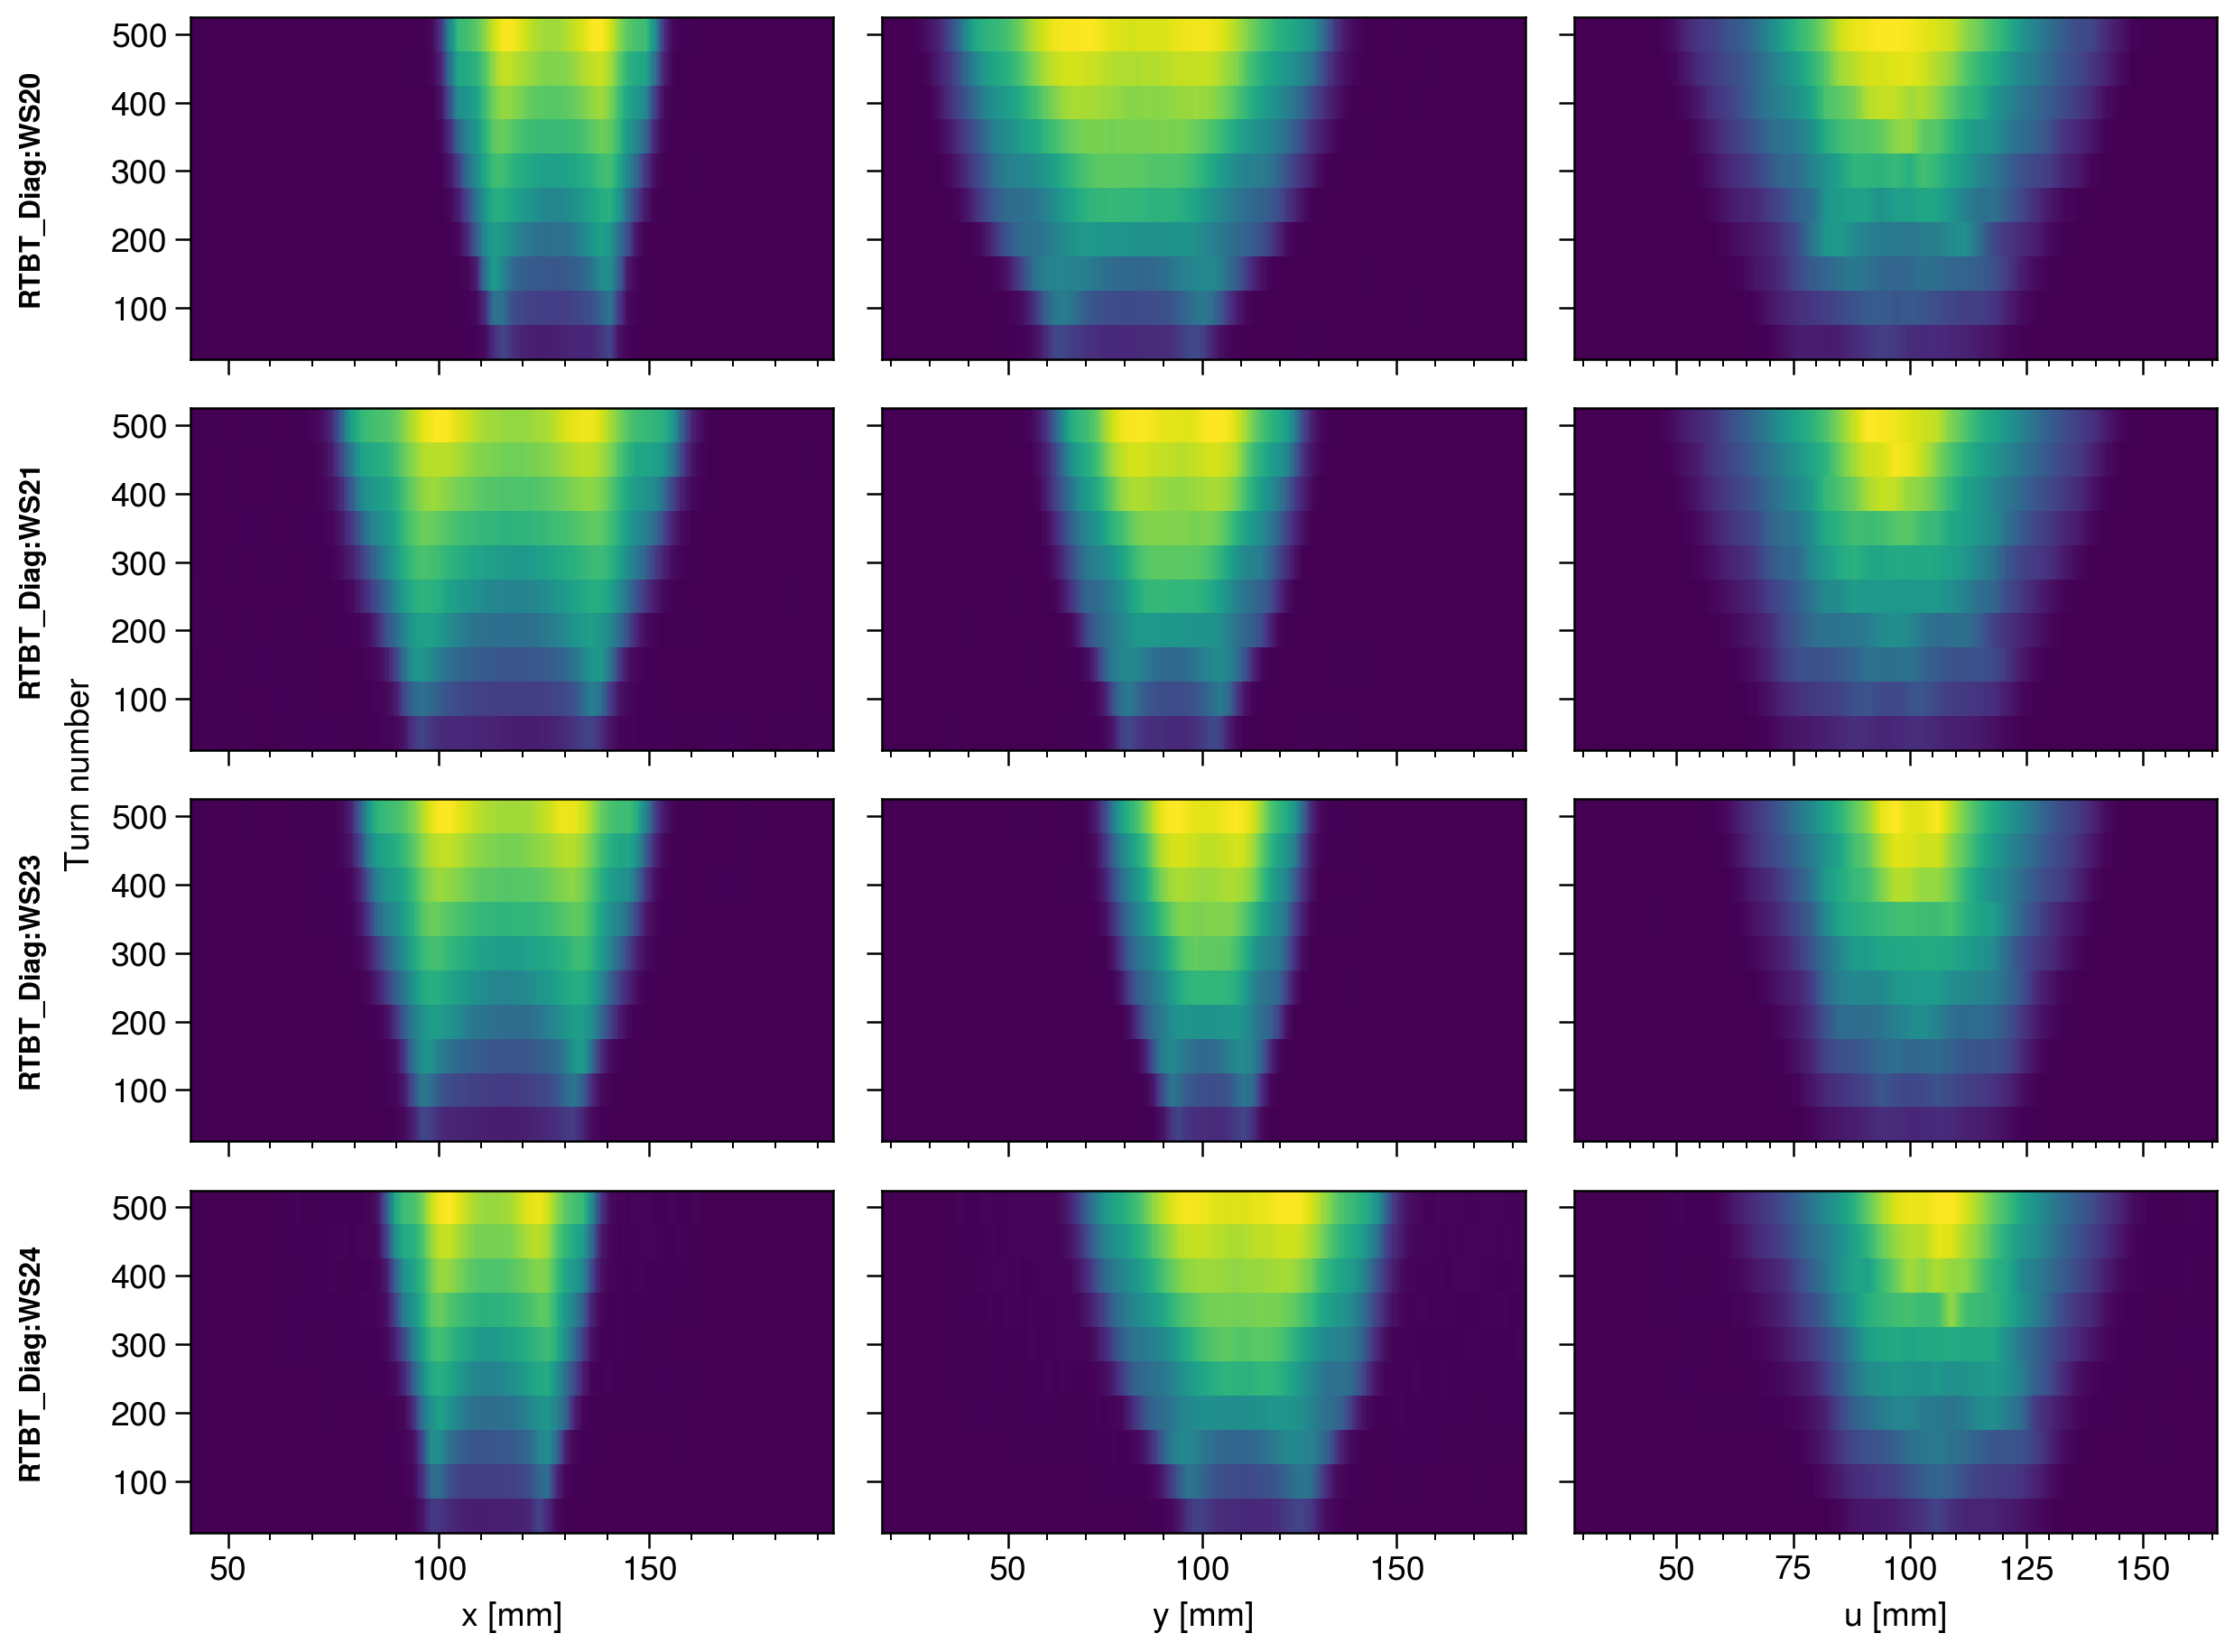
\includegraphics[width=\textwidth]{Images/chapter5/exp1a/waterfall.png}
    \end{subfigure}
    \vfill
    \vspace*{1.25cm}
    \vfill
    \begin{subfigure}{\textwidth}
        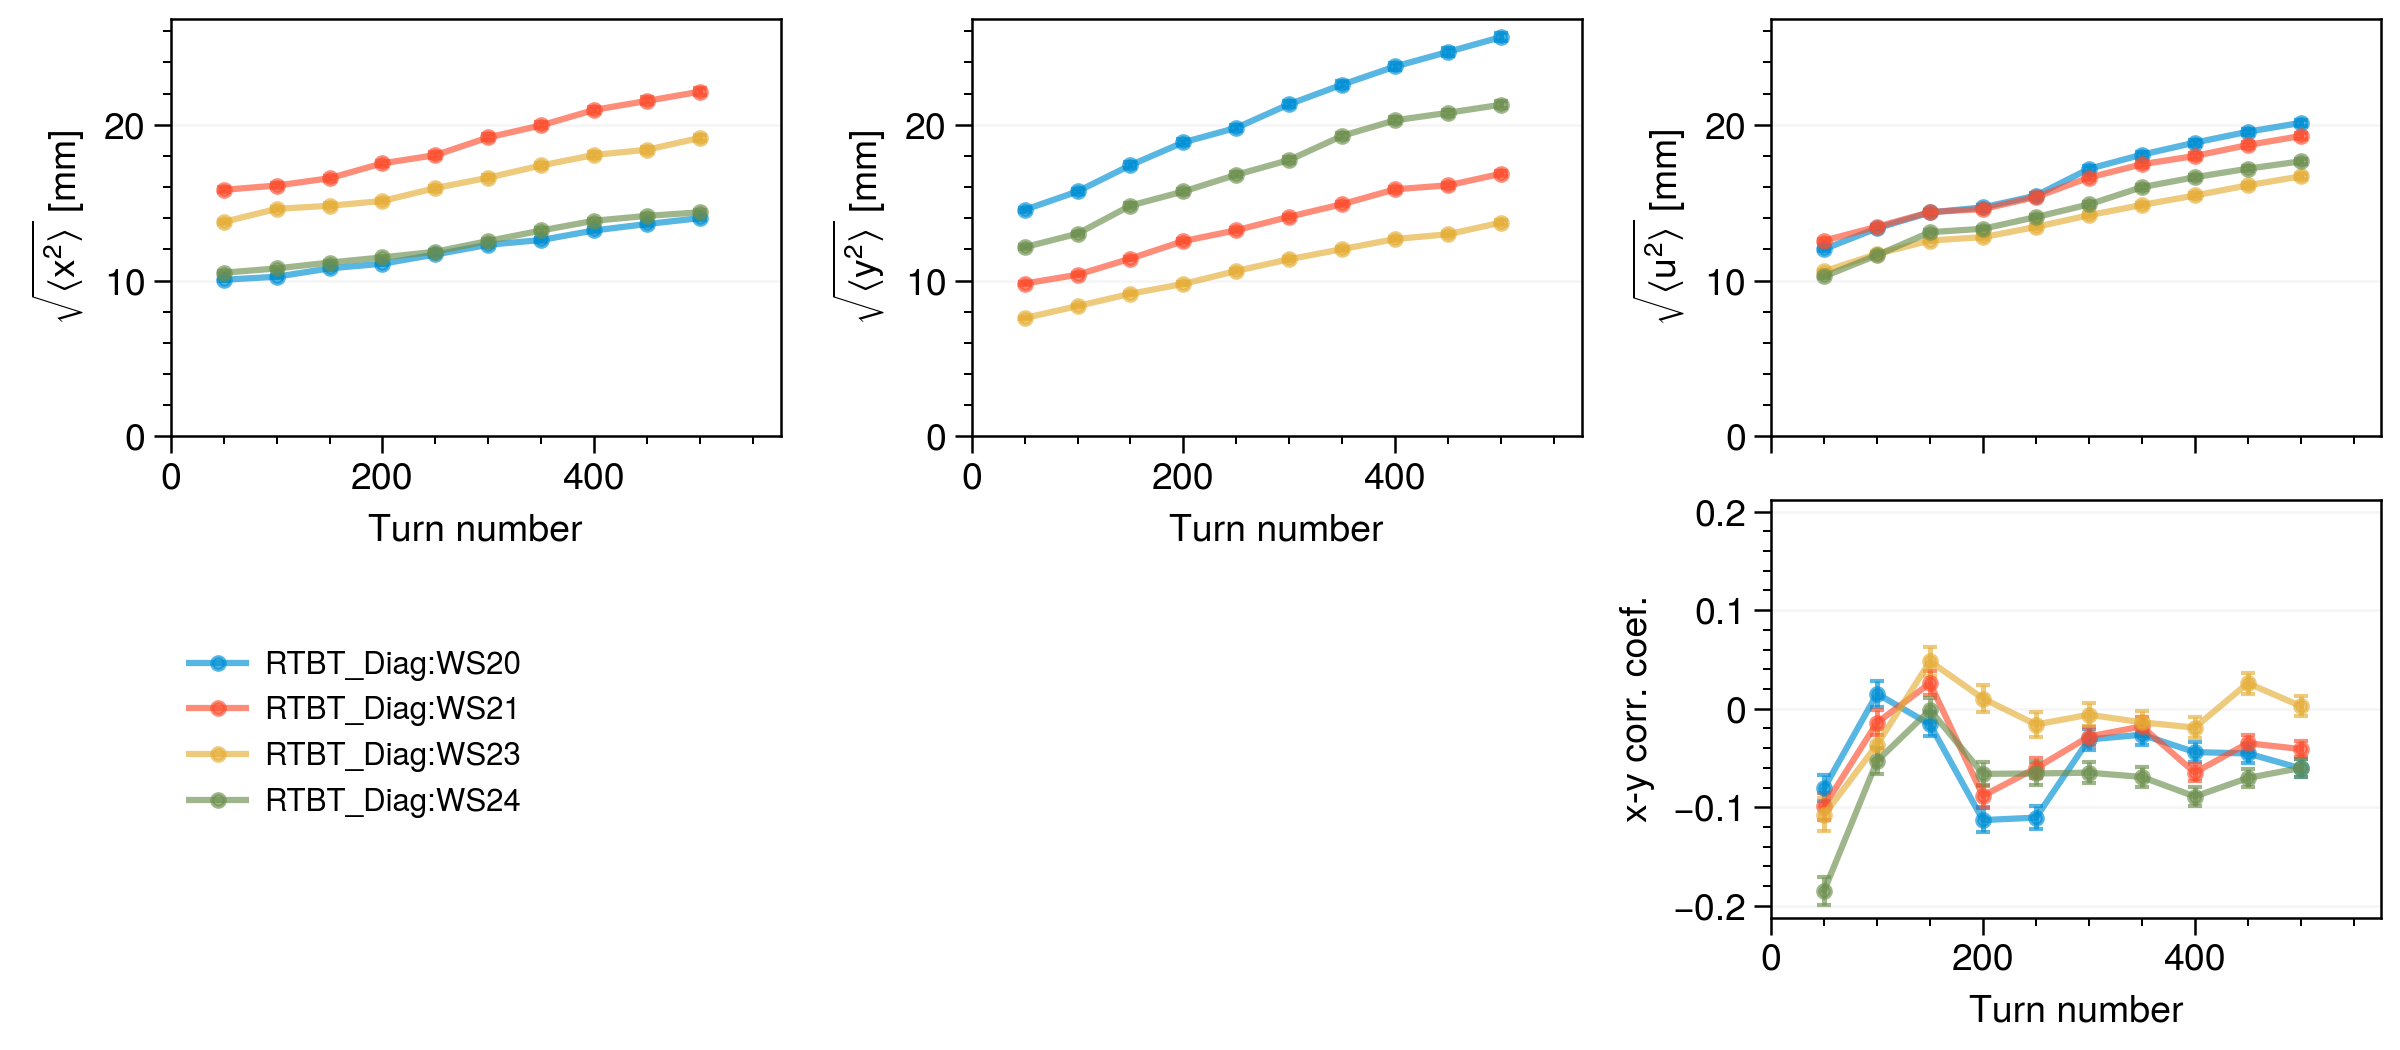
\includegraphics[width=\textwidth]{Images/chapter5/exp1a/rms.png}
    \end{subfigure}
    \caption{Measured wire-scanner profiles from Experiment 1a. The top figure shows the measured profiles on each wire as a function of time. The bottom plots show the moments extracted from the profiles.}
    \label{fig:exp1a_wsmeas}
\end{figure}
%
%
\begin{figure}[!p]
    \centering
    \begin{subfigure}{0.6\textwidth}
        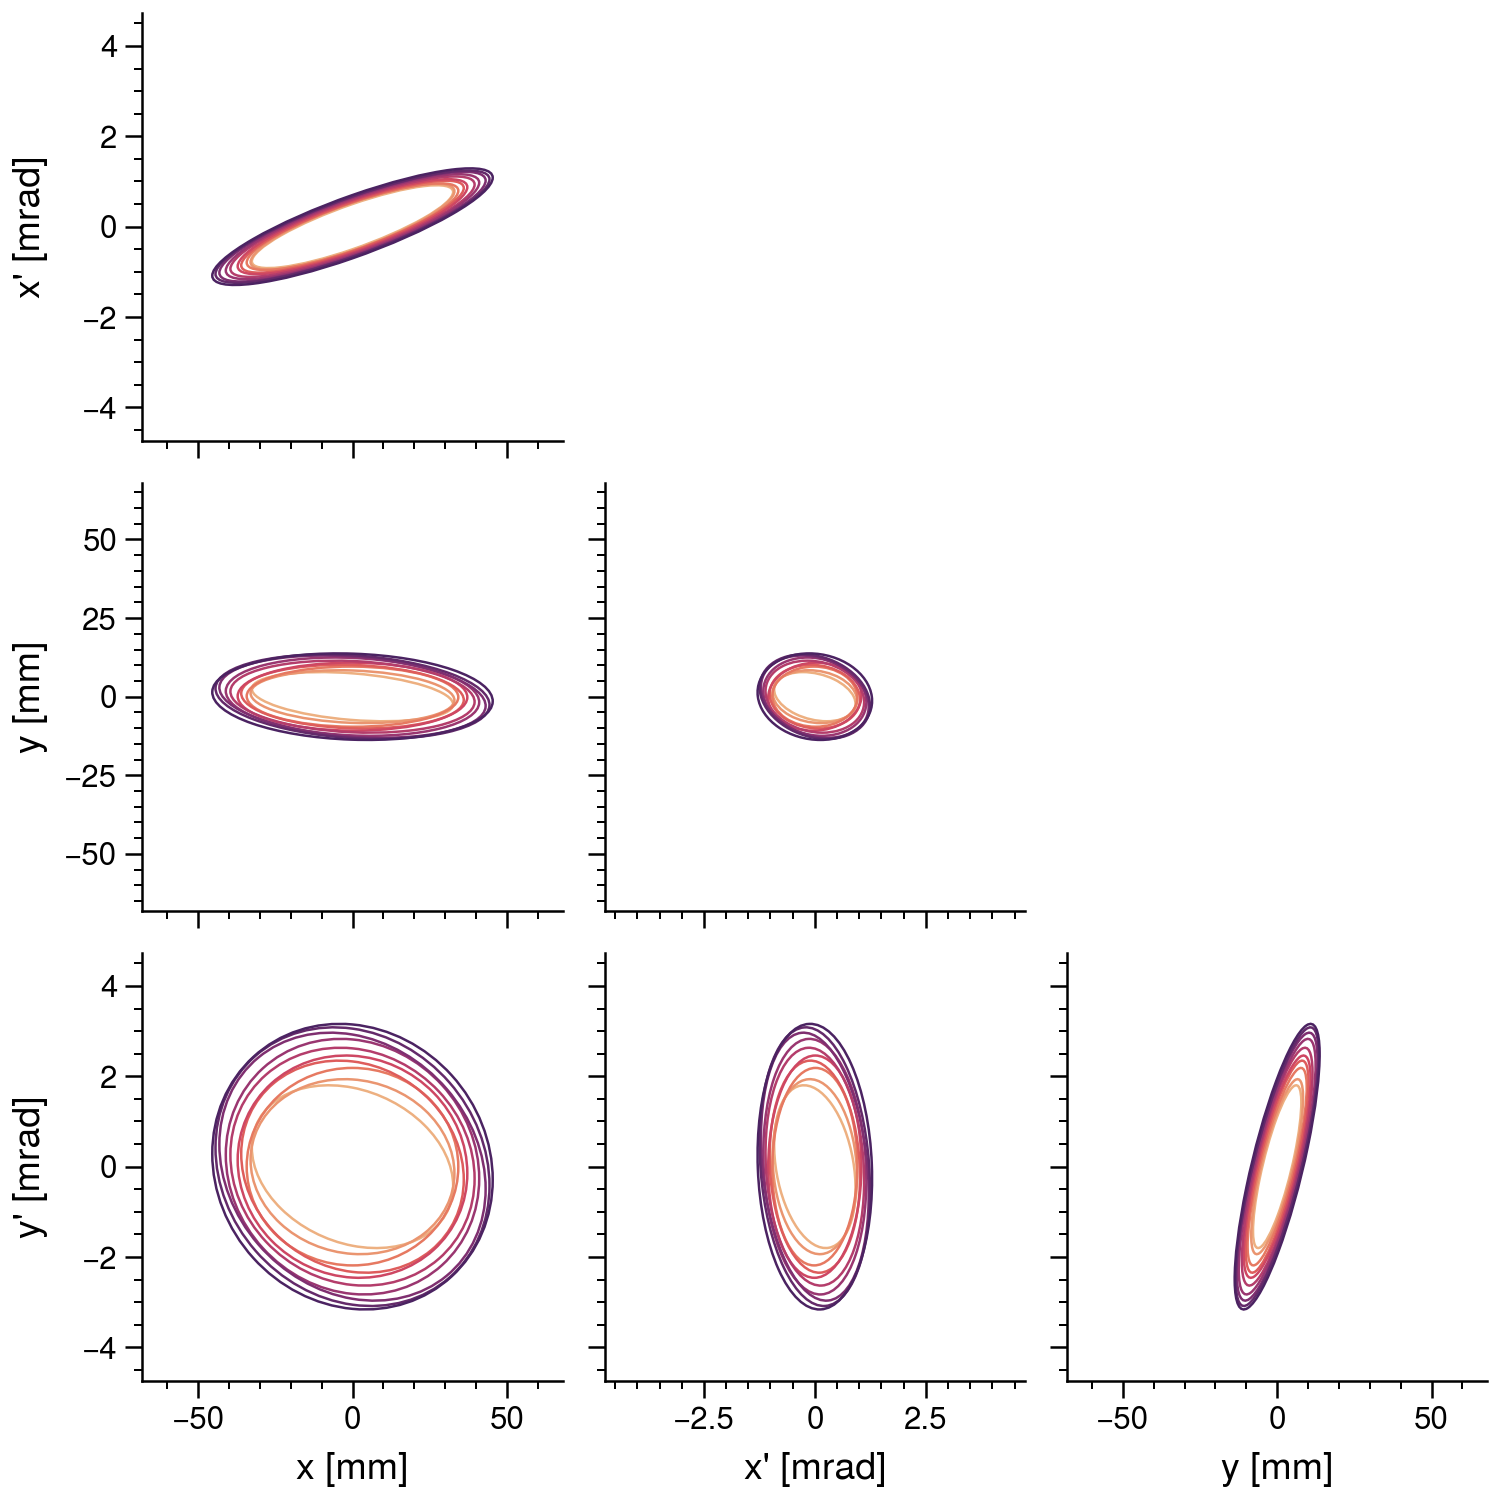
\includegraphics[width=\textwidth]{Images/chapter5/exp1a/corner.png}
    \end{subfigure}
    \hfill
    \begin{subfigure}[t]{0.39\textwidth}
        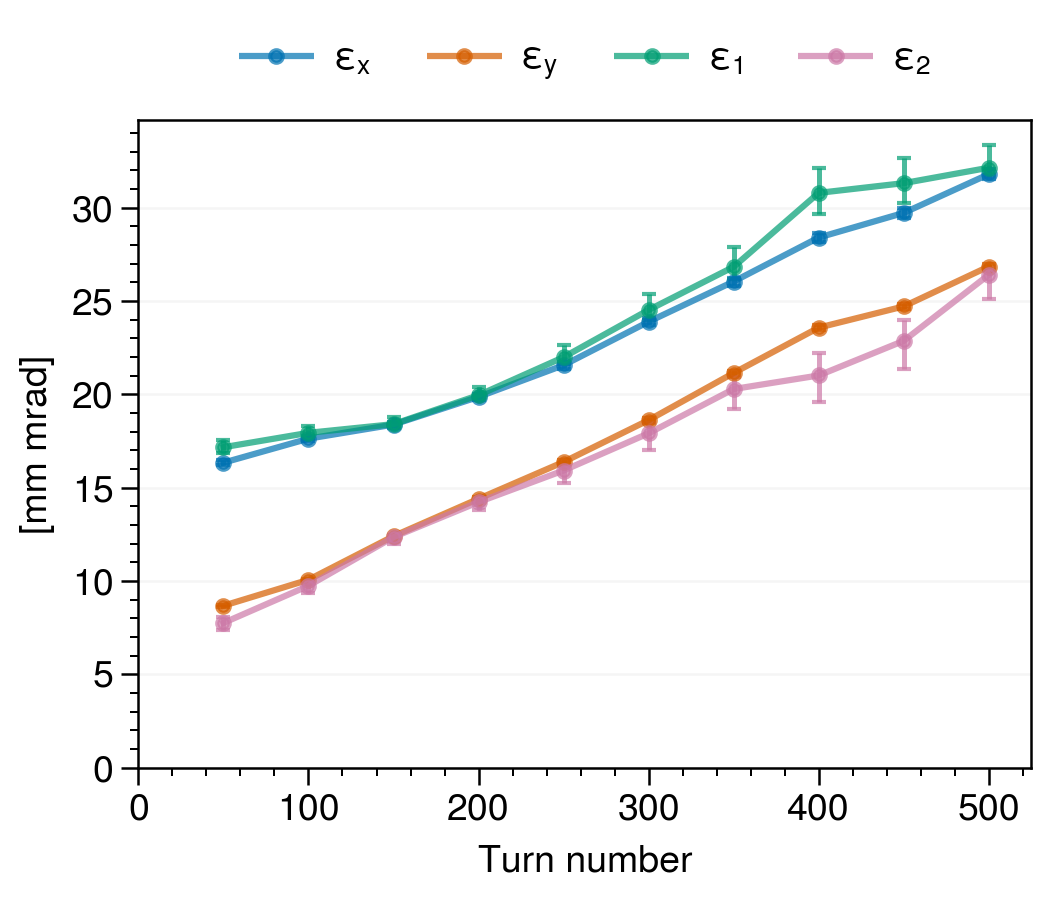
\includegraphics[width=\textwidth]{Images/chapter5/exp1a/emittances.png}
    \end{subfigure}
    \caption{Reconstructed emittances and covariance ellipses from Experiment 1a. In this and subsequent figures, the reconstruction is performed at BPM17 and the light/dark ellipses correspond to the start/end of injection.}
    \label{fig:exp1a_emittances}
\end{figure}
%
Each subplot shows the evolution of the projection onto a single wire; each row corresponds to a different wire-scanner and each column to a different projection axis — $x$, $y$, or $u$. Recall that in correlated painting, the injection angles are zero and the positions are increased from an initial offset. The initial offset is evident from the two peaks in the measured $x$ and $y$ profiles. The hollow center of the distribution eventually fills in due to nonlinear effects.

The reconstructed emittances and covariance ellipses at BPM17, just before QH18, are shown in Fig.~\ref{fig:exp1a_emittances}. The size and location of the error bars were computed by repeating the reconstruction multiple times with 3\% random noise added to the measured moments, then taking the mean and standard deviation over the trials. For our purposes, the most important feature of Fig.~\ref{fig:exp1a_emittances} is that the measured cross-plane correlation is small throughout injection, demonstrating that there is very little coupling from electromagnetic fields of the beam or ring in the standard SNS painting scheme.


\subsection{Experiment 1b: attempted elliptical painting}

We then attempted elliptical painting. First, the horizontal and vertical tunes were set to 6.18. The next step was to move the closed orbit to the foil, which was found to be possible in the vertical plane but impossible in the horizontal plane. The minimum horizontal distance from the foil was 10 mm, and the maximum vertical injection angle was 0.7 mrad; assuming $\alpha_y \approx 0$ and $\beta_y \approx 10$, the painted vertical emittance can be estimated as
%
\begin{equation}
\begin{aligned}
    \varepsilon_y 
    &\approx \frac{1}{4}\beta_y {y_{max}'}^2
    = 1.22 \,\, \text{mm~mrad},
\end{aligned}
\end{equation}
%
which is only four times larger than the emittance from the linac. Although this is not ideal, we continued using initial coordinates ($x$, $x'$, $y$, $y'$) $\approx$ (10 mm, 0 mrad, 0 mm, 0 mrad) and final coordinates ($x$, $x'$, $y$, $y'$) $\approx$ (21 mm, 0 mrad, 0 mm, 0.7 mrad).

Let us pause to predict the beam evolution using these settings, assuming linear transport: initial particles would oscillate along a flat horizontal ellipse in the $x$-$y$ plane, and as time progressed, the horizontal and vertical size of the ellipse would grow at different rates depending on the maximum injected $x$ and $y'$ coordinates. The inclusion of space charge complicates the analysis due to the non-uniformity introduced by the initial horizontal offset. 

The measured wire-scanner profiles are shown in Fig.~\ref{fig:exp1b_wsmeas}.
%
\begin{figure}[!p]
    \centering
    \begin{subfigure}{\textwidth}
        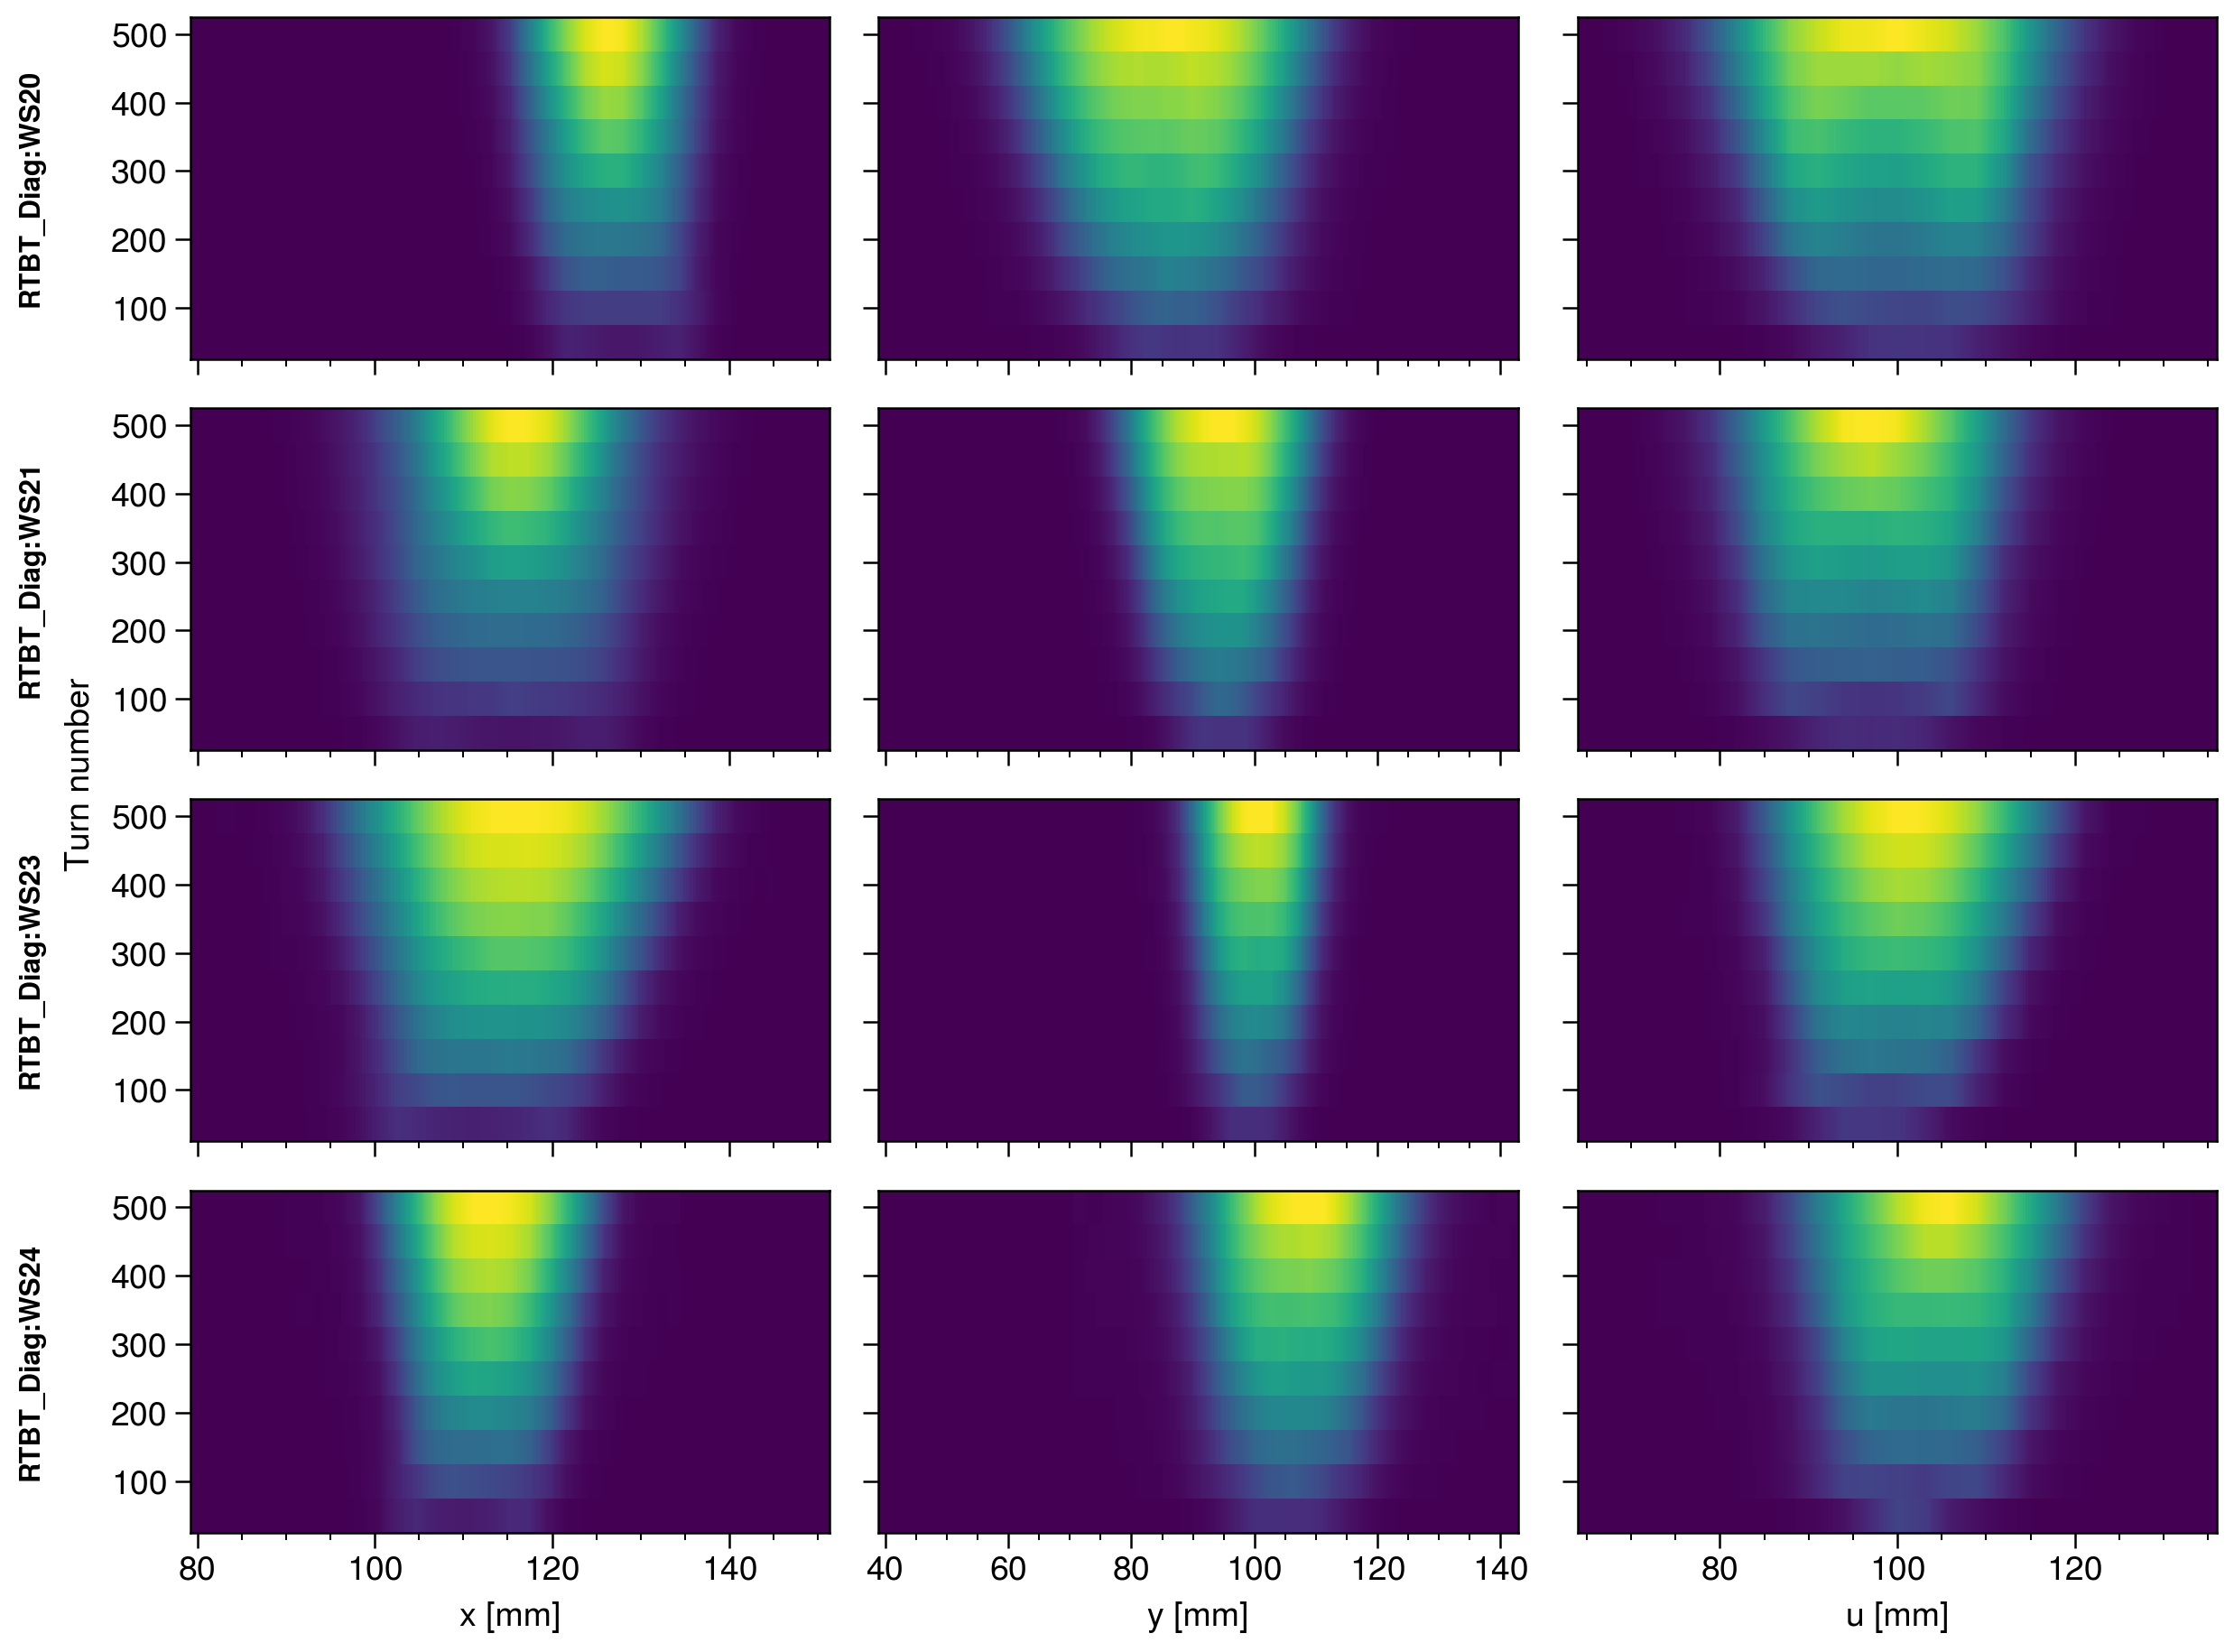
\includegraphics[width=\textwidth]{Images/chapter5/exp1b/waterfall.png}
    \end{subfigure}
    \vfill
    \vspace*{1.25cm}
    \vfill
    \begin{subfigure}{\textwidth}
        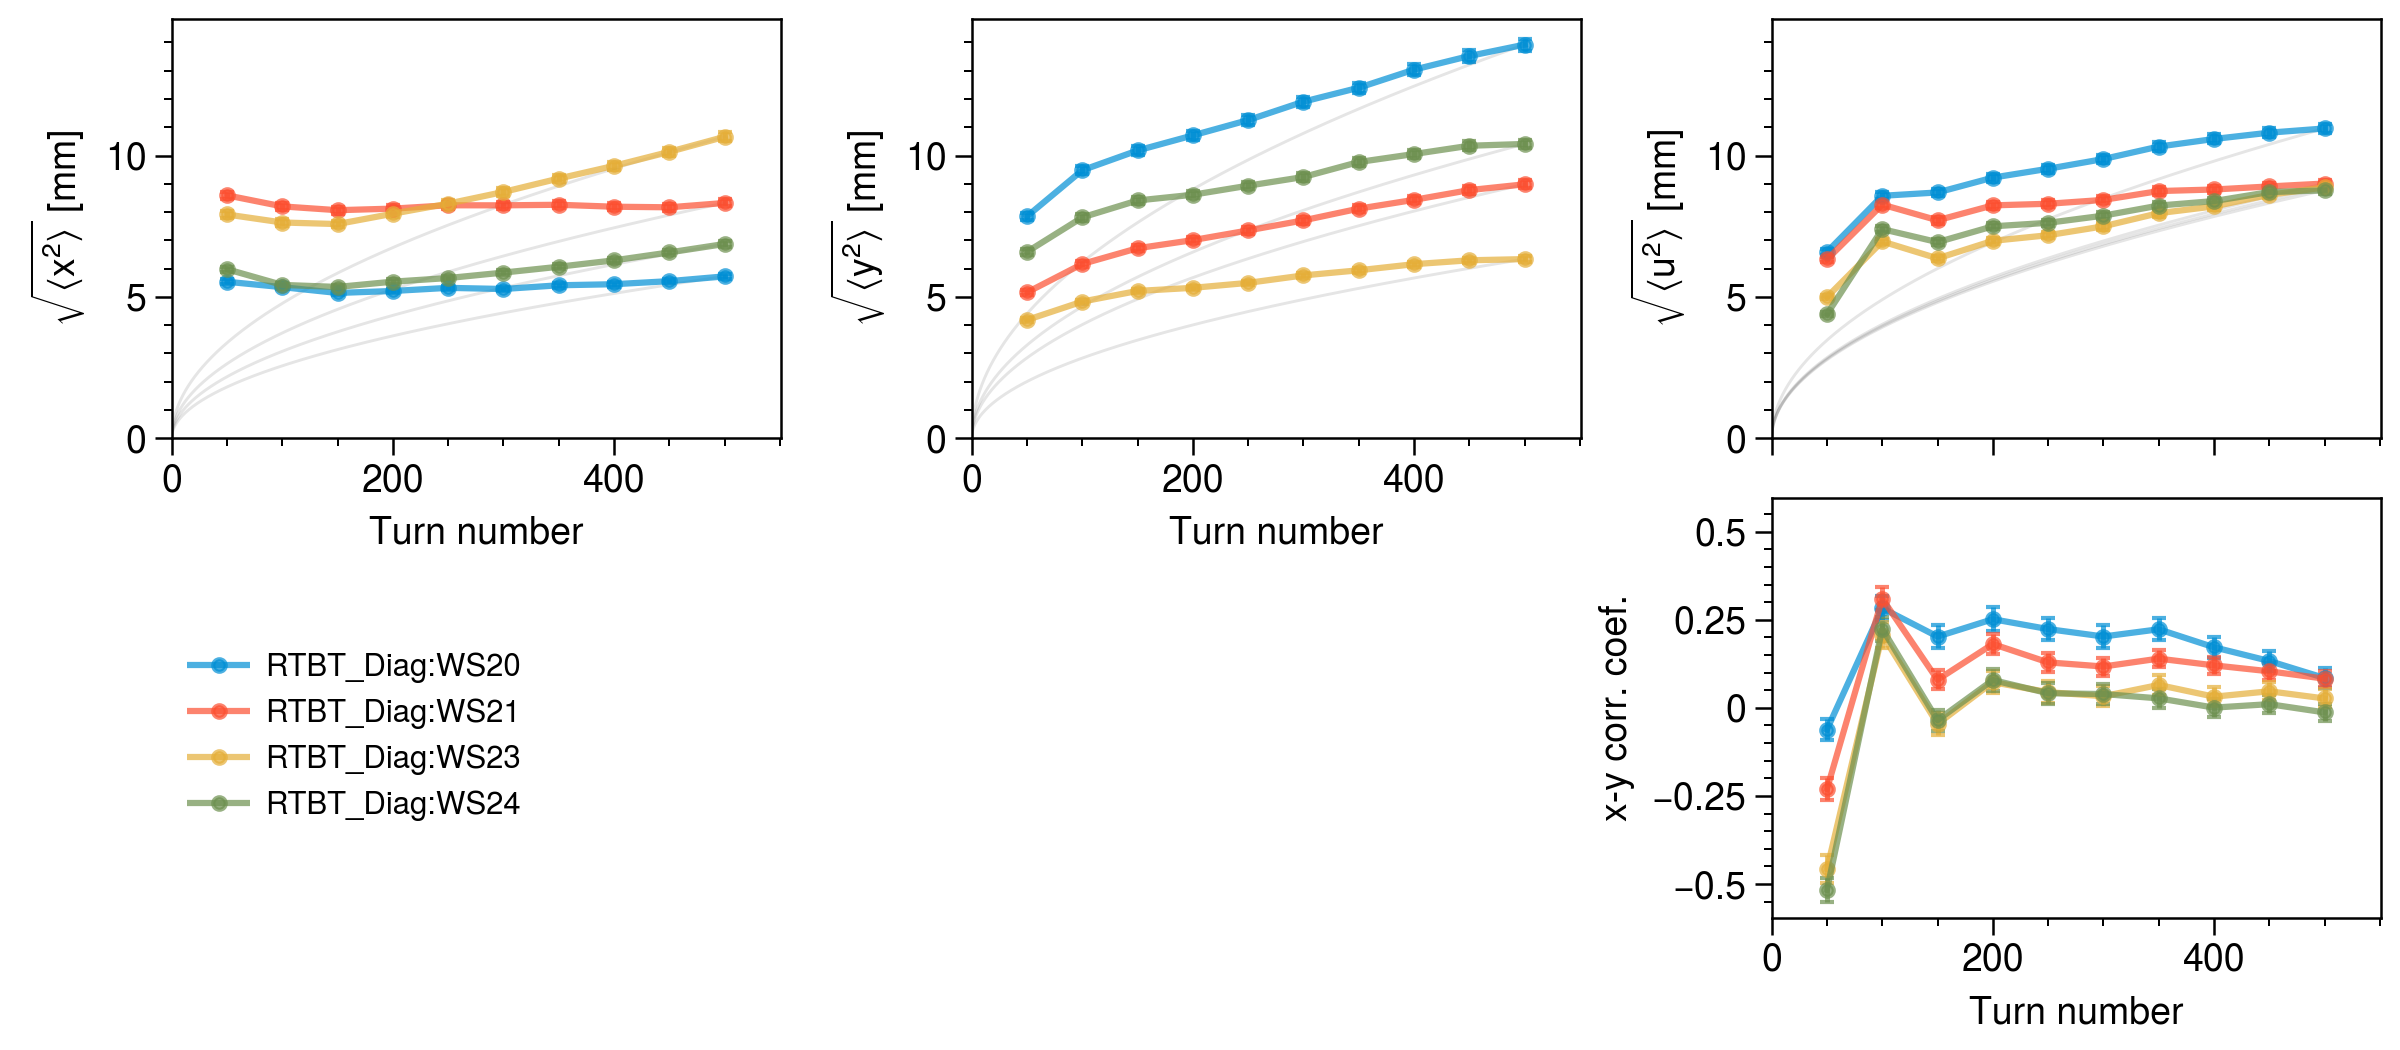
\includegraphics[width=\textwidth]{Images/chapter5/exp1b/rms.png}
    \end{subfigure}
    \caption{Measured wire-scanner profiles from Experiment 1b.}
    \label{fig:exp1b_wsmeas}
\end{figure}
%
The horizontal projection at 50 turns is hollow — evidence of the initial offset of the closed orbit — but quickly filaments. The most important feature of Fig.~\ref{fig:exp1b_wsmeas} is the vertical beam size, which starts at a small value and increases throughout injection. This is an indication that the injection kicker waveforms are correct. Notice that the beam is much smaller than in Experiment 1a.

We now turn to the reconstructed emittances and covariance ellipses in Fig.~\ref{fig:exp1b_emittances}.
%
\begin{figure}[!p]
    \centering
    \begin{subfigure}{0.6\textwidth}
        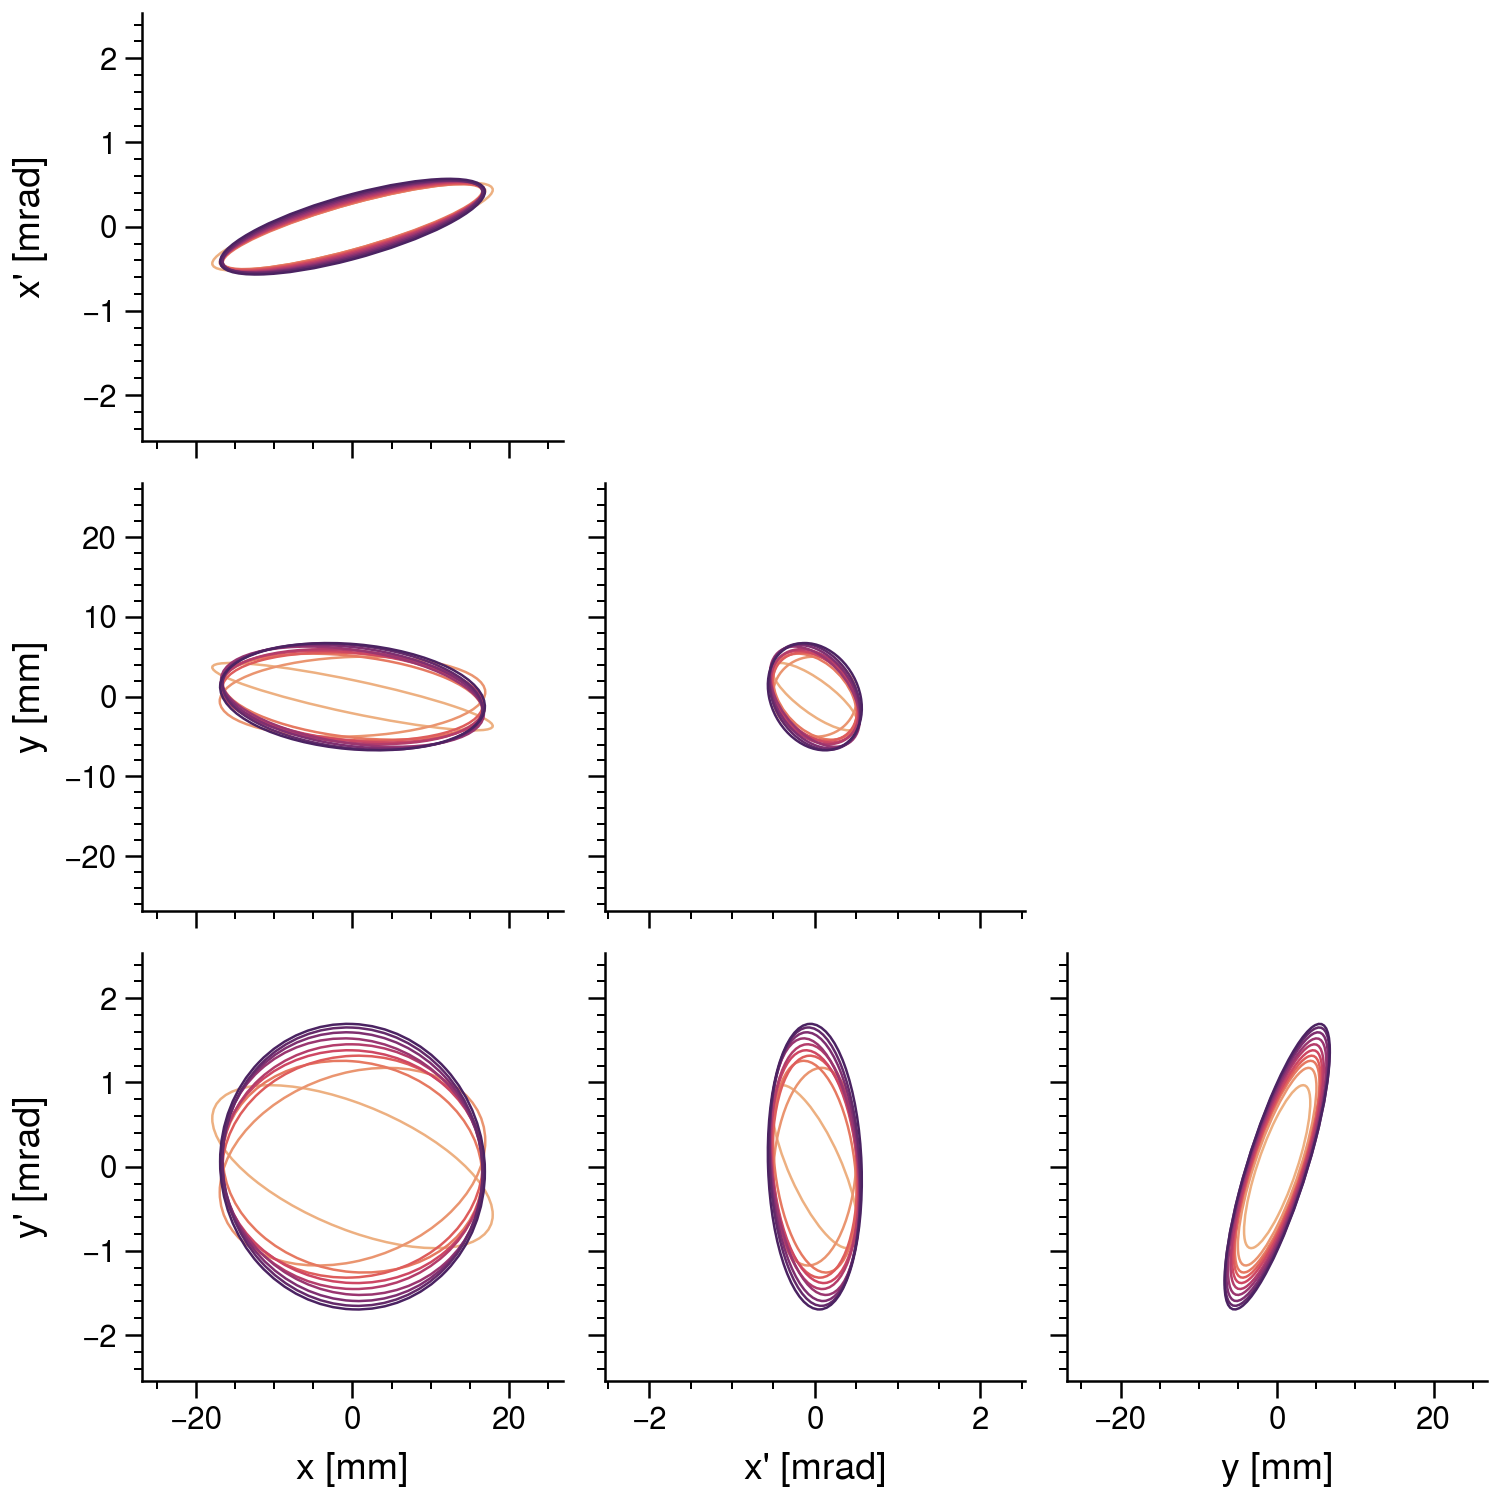
\includegraphics[width=\textwidth]{Images/chapter5/exp1b/corner.png}
    \end{subfigure}
    \hfill
    \begin{subfigure}[t]{0.39\textwidth}
        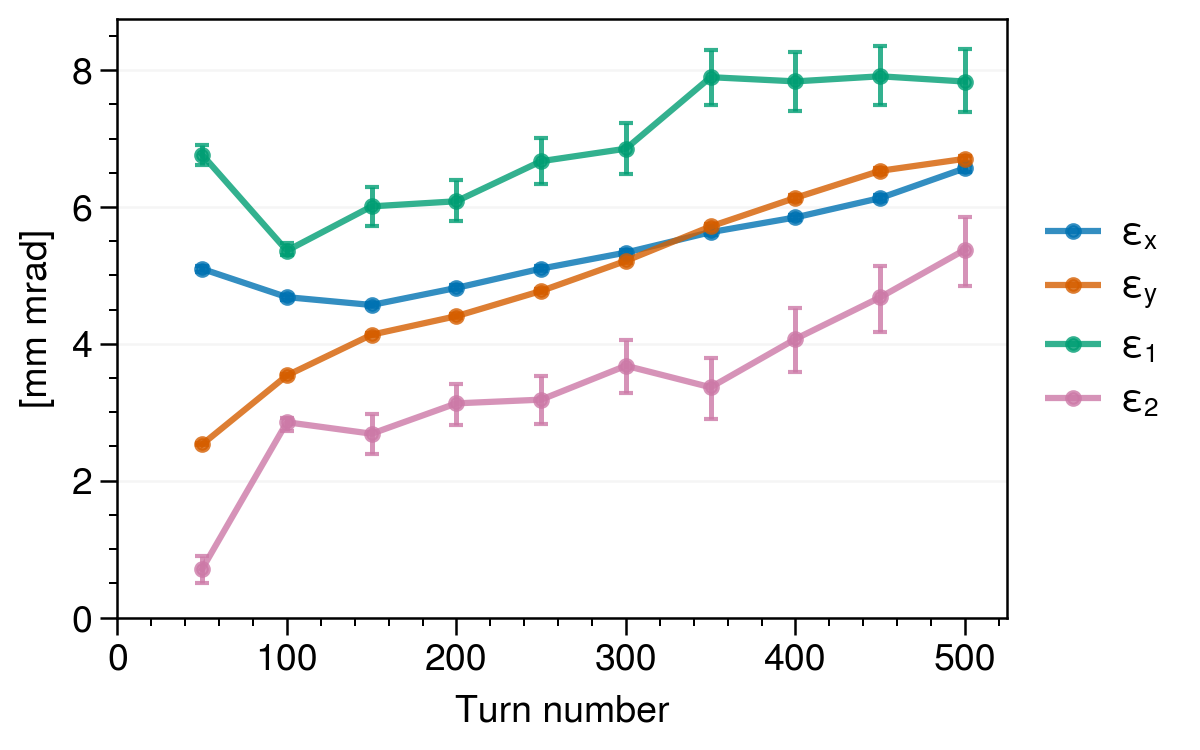
\includegraphics[width=\textwidth]{Images/chapter5/exp1b/emittances.png}
    \end{subfigure}
    \caption{Reconstructed emittances and covariance ellipses from Experiment 1b.}
    \label{fig:exp1b_emittances}
\end{figure}
%
There is a clear separation between the intrinsic and apparent emittances throughout accumulation. A possible explanation for the larger-than-expected increase in vertical emittance is that space charge coupled the motion during injection, causing emittance exchange as new particles were added to the bunch; another possible explanation is emittance blow-up due to many particles being injected into a small region of vertical phase space; the answer is left for future work. The most important feature of Fig.~\ref{fig:exp1b_emittances} is that the measured distribution was significantly different than in the previous experiment and was closer to the desired case; in other words, the ring modifications seem to have worked as intended. We close with a PyORBIT simulation of this experiment in Fig.~\ref{fig:exp1b_sim}. 
%
\begin{figure}[!p]
    \centering
    \begin{subfigure}{\textwidth}
        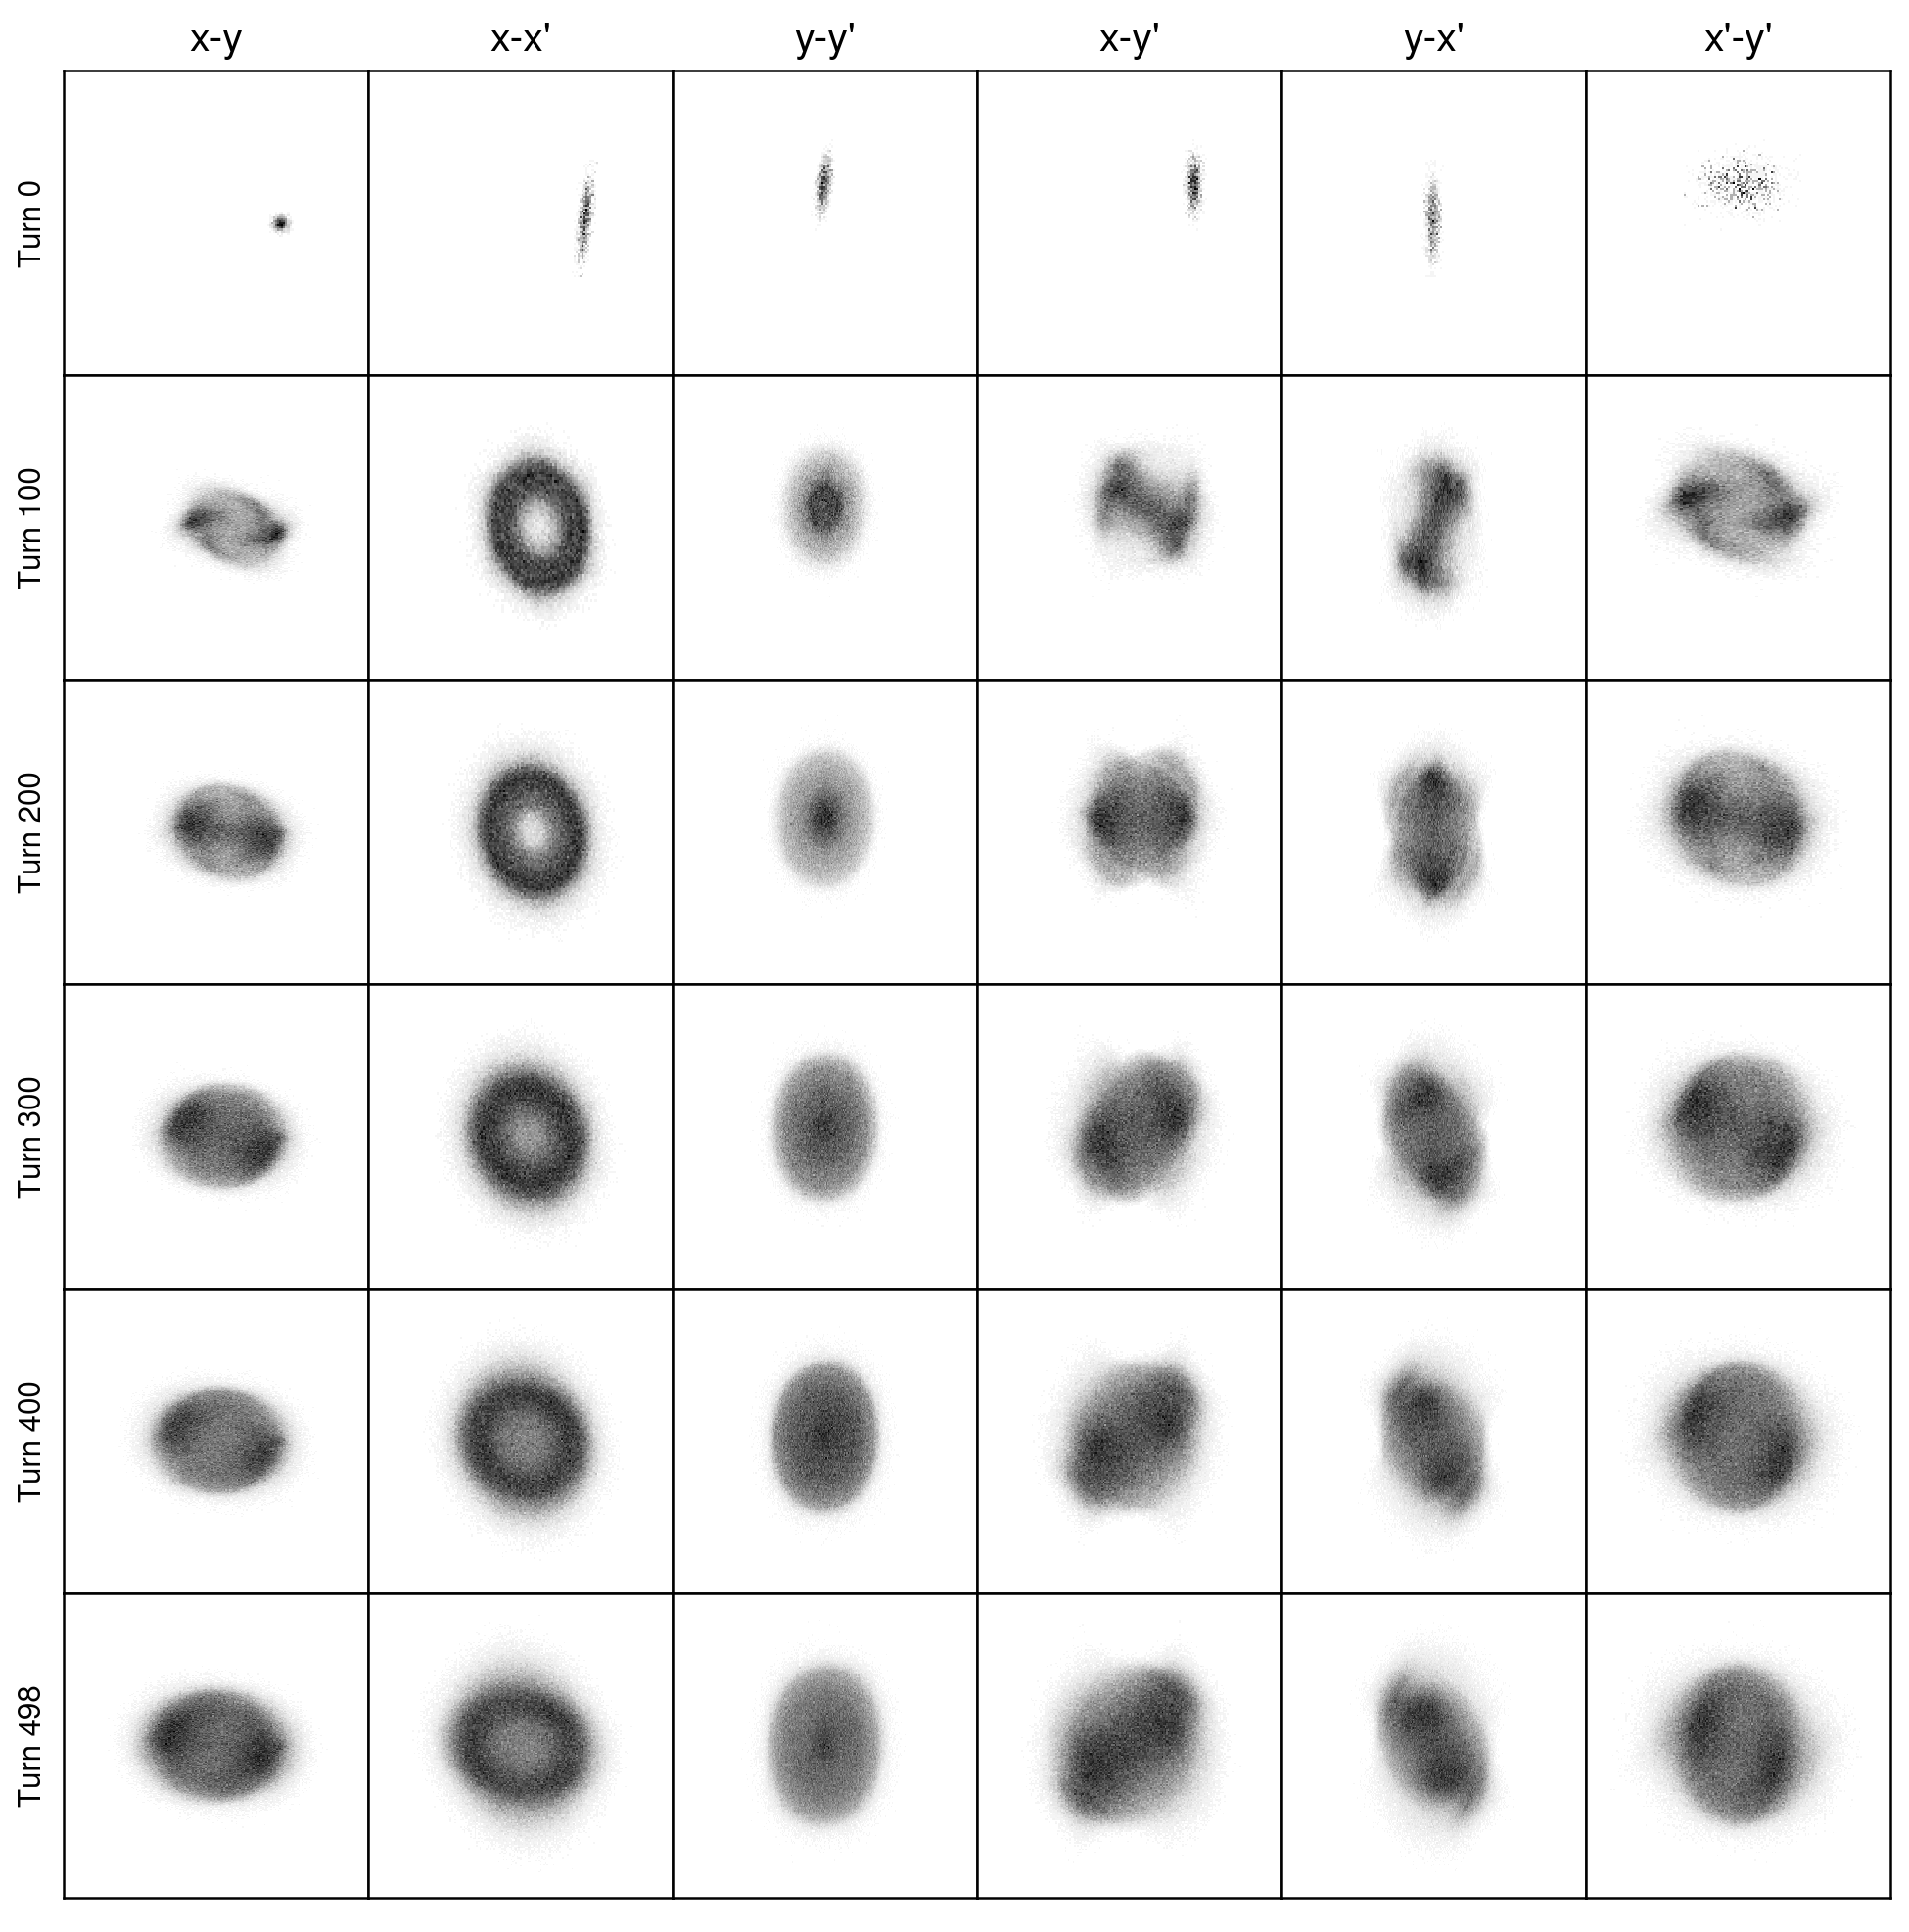
\includegraphics[width=\textwidth]{Images/chapter5/exp1b/sim_snapshots.png}
    \end{subfigure}
    \vfill
    \vspace*{1.0cm}
    \vfill
    \begin{subfigure}{0.7\textwidth}
        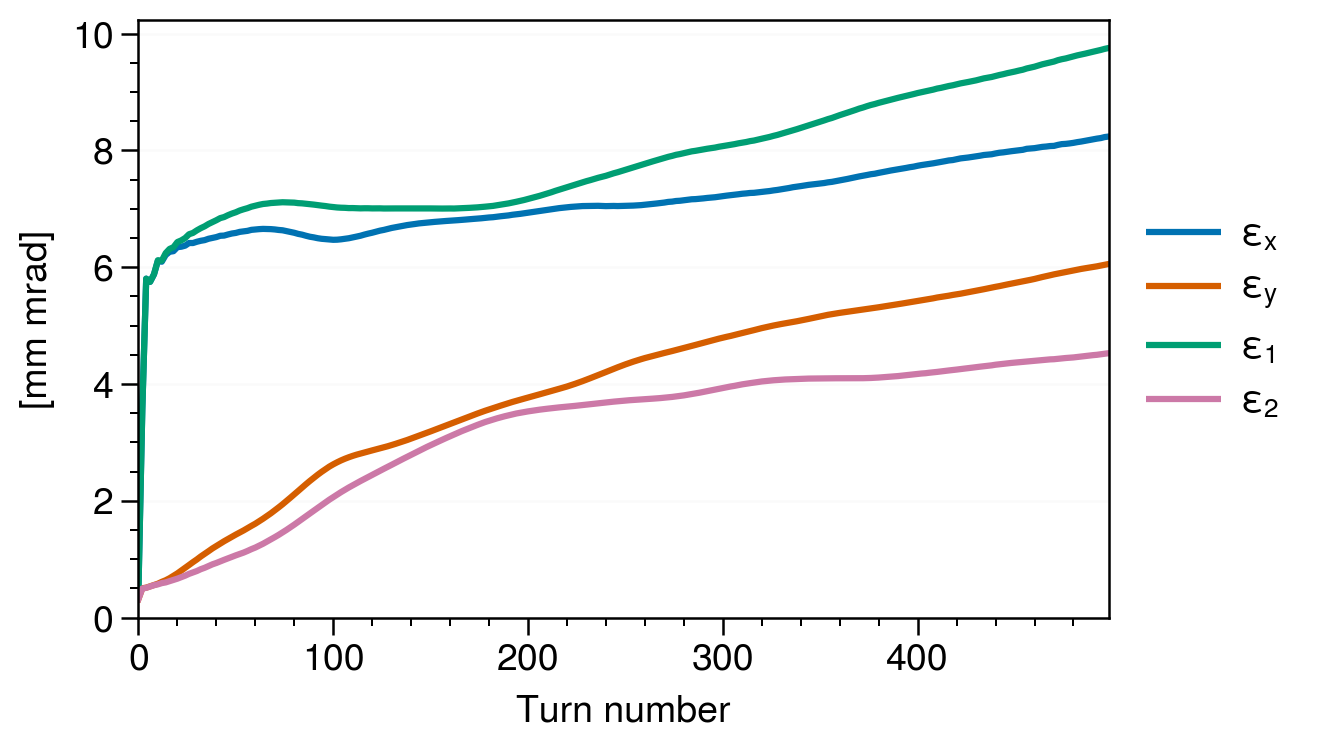
\includegraphics[width=\textwidth]{Images/chapter5/exp1b/sim_emittances.png}
    \end{subfigure}
    \caption{Simulation of Experiment 1b.}
    \label{fig:exp1b_sim}
\end{figure}
%
Keep in mind that the $\beta$ functions of the ring at the injection point are not the same as in the experiment, so the exact values of the emittances are not expected to agree. Qualitative agreement with the measured emittance growth appears to be present.



\section{Experiment 2}

In Experiment 2, the beam energy was lowered to 0.8 GeV. At this energy, the closed orbit was able to reach the foil with zero slope, i.e., $x = x' = y = y' = 0$, as required to paint a uniform density beam. Again, only $x$ and $y'$ need to change during injection. There is no limit on $x_{max}$ since increasing $x$ involves decreasing the horizontal kickers, but the vertical kickers could only reach $y'_{max} \approx 1.1$ mrad. In the linear approximation, this angle is expected to produce a vertical emittance of 3-4 mm~mrad. We estimate the ratio of painted emittances as
%
\begin{equation}\label{eq:painted_emittance_ratio}
    \frac{\varepsilon_y}{\varepsilon_x} \approx 
    \beta_x \beta_y \left(\frac{{y_{max}}'}{x_{max}}\right)^2 
    .
\end{equation}
%
To paint equal emittances would require $x_{max}$ $\approx$ 10 mm — a small beam. We decided to use $x_{max}$ = 21 mm, maintaining the same beam intensity as in Experiment 1. 

The measured wire-scanner profiles are shown in Fig.~\ref{fig:exp2_wsmeas}.
%
\begin{figure}[!p]
    \centering
    \begin{subfigure}{\textwidth}
        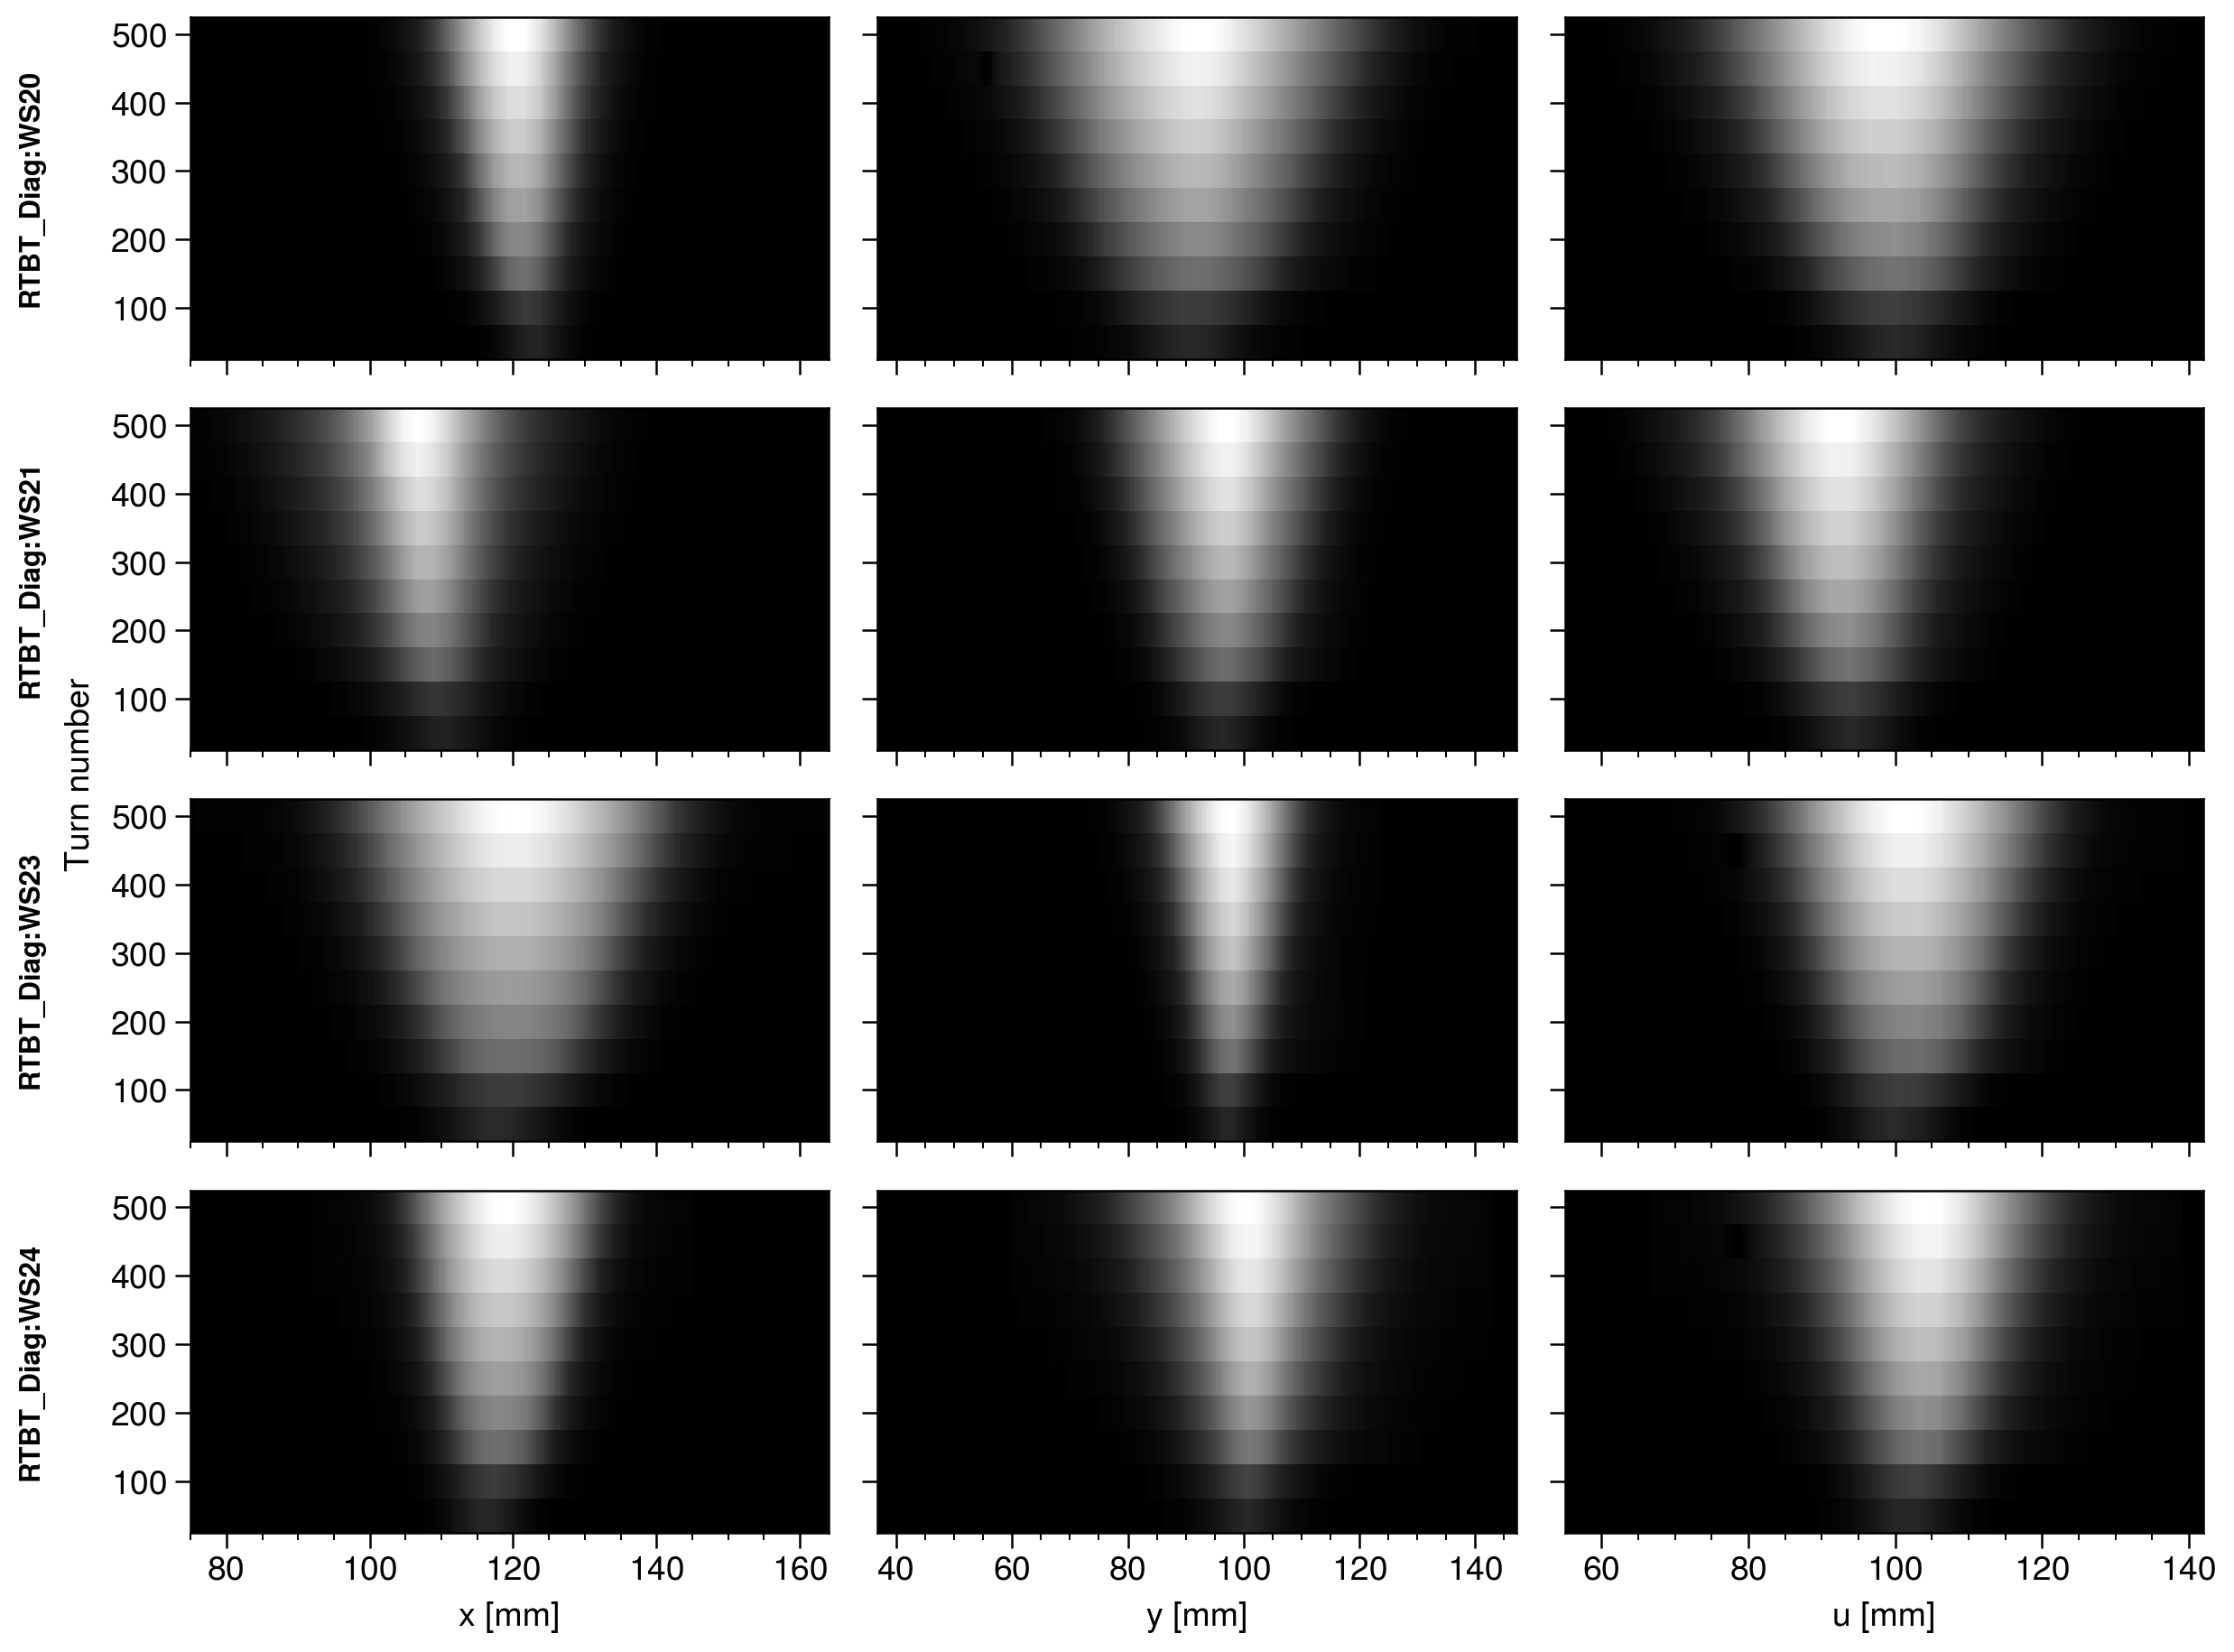
\includegraphics[width=\textwidth]{Images/chapter5/exp2/waterfall.png}
    \end{subfigure}
    \vfill
    \vspace*{1.25cm}
    \vfill
    \begin{subfigure}{\textwidth}
        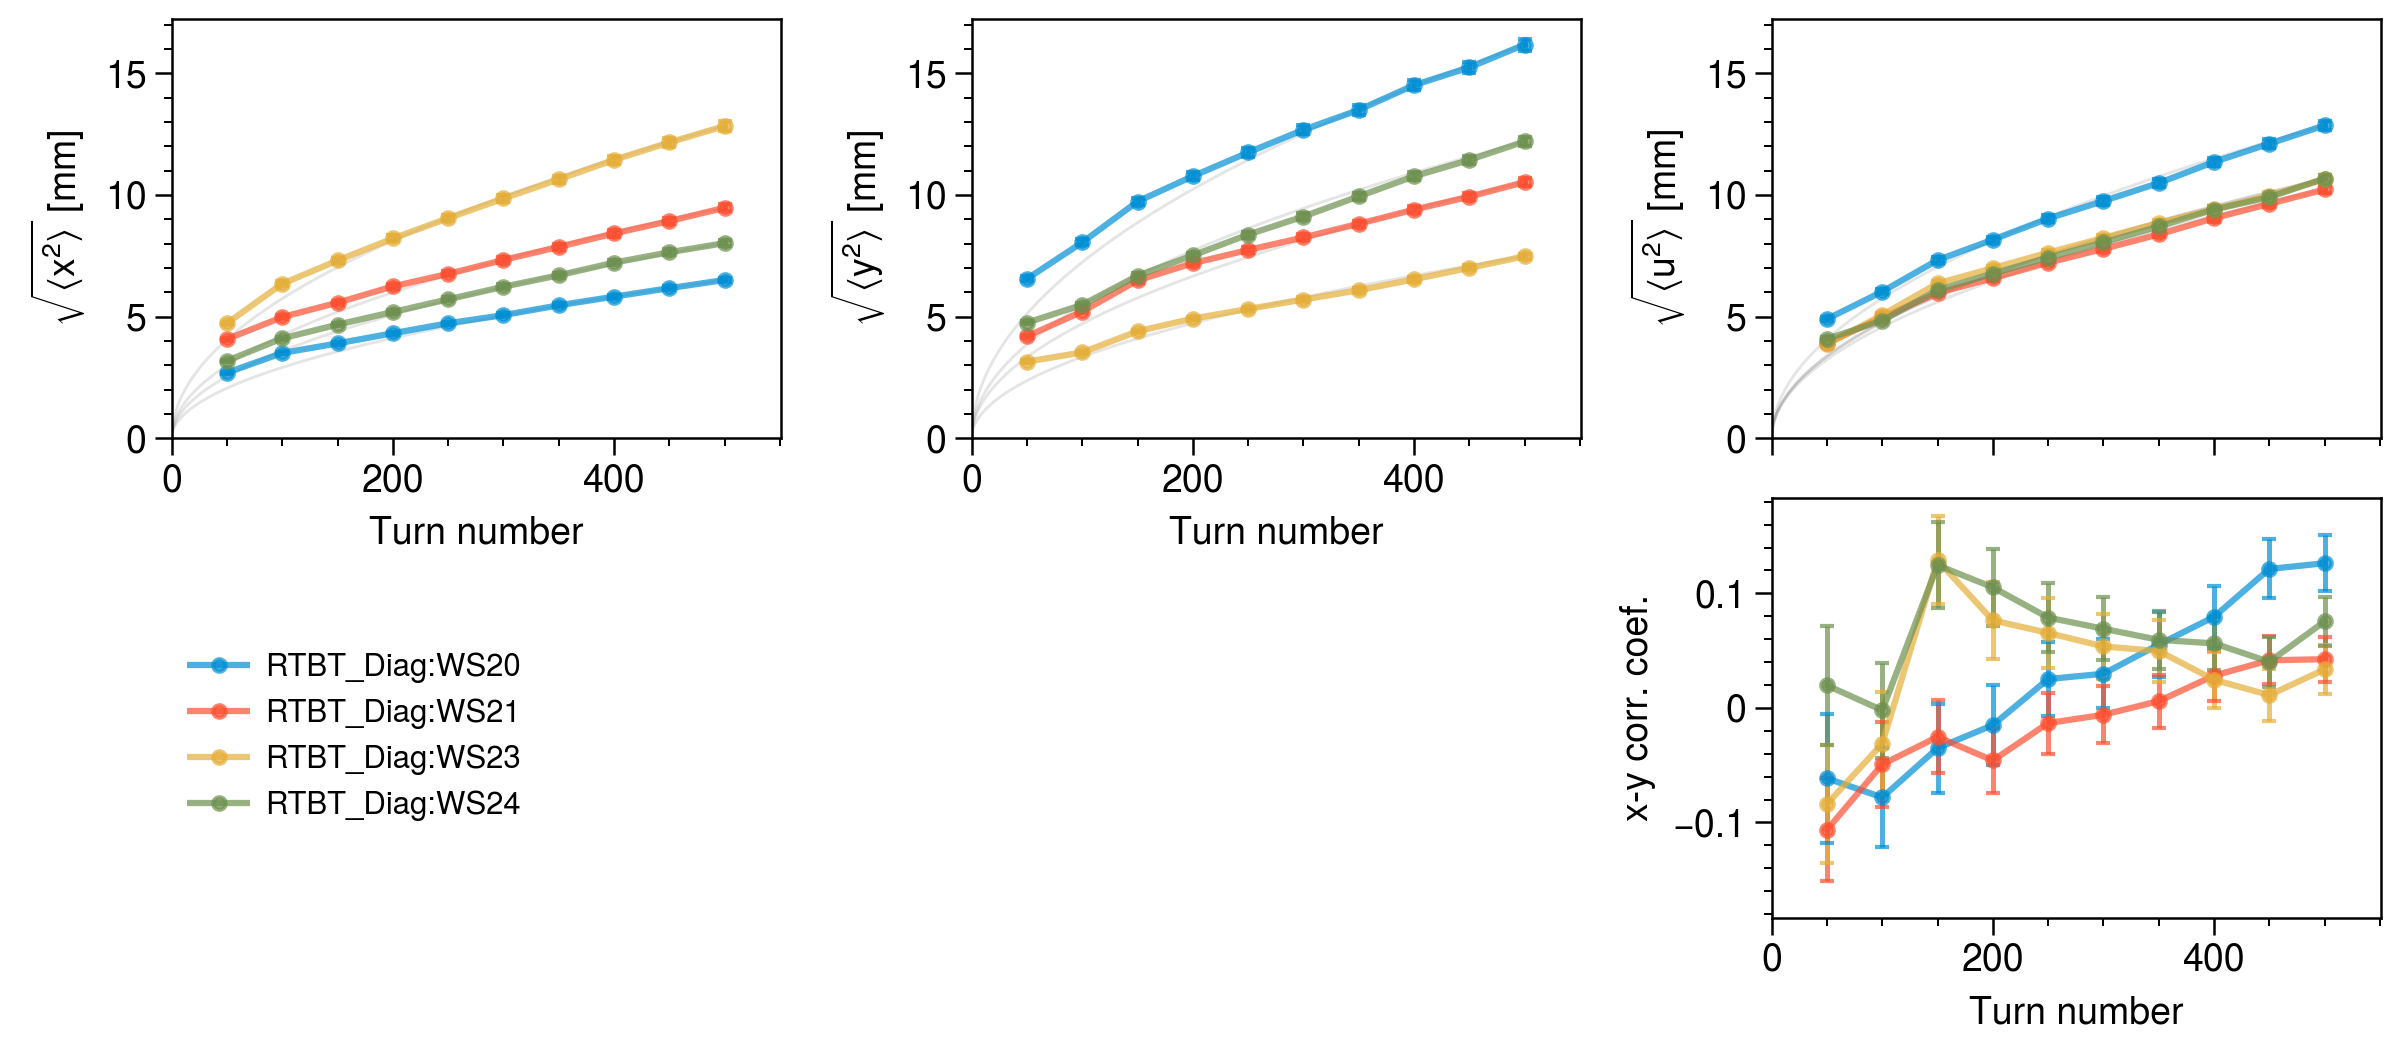
\includegraphics[width=\textwidth]{Images/chapter5/exp2/rms.png}
    \end{subfigure}
    \caption{Measured wire-scanner profiles during injection from Experiment 2.}
    \label{fig:exp2_wsmeas}
\end{figure}
%
One important feature of Fig.~\ref{fig:exp2_wsmeas} is that the beam must have some rotational symmetry in the $x$-$y$ plane since the growth in beam size is similar on all wires. A second important feature is that the beam sizes start at a small value and increase at approximately the square root of time (light grey curves have been added showing the ideal square root time dependence given the final beam size). A third important feature is that the profiles appear to be more consistent with a Gaussian distribution than a uniform density distribution. This will be discussed more at the end of the chapter.

The reconstructed emittances and covariance ellipses are shown in Fig.~\ref{fig:exp2_emittances}.
%
\begin{figure}[!p]
    \centering
    \begin{subfigure}{0.6\textwidth}
        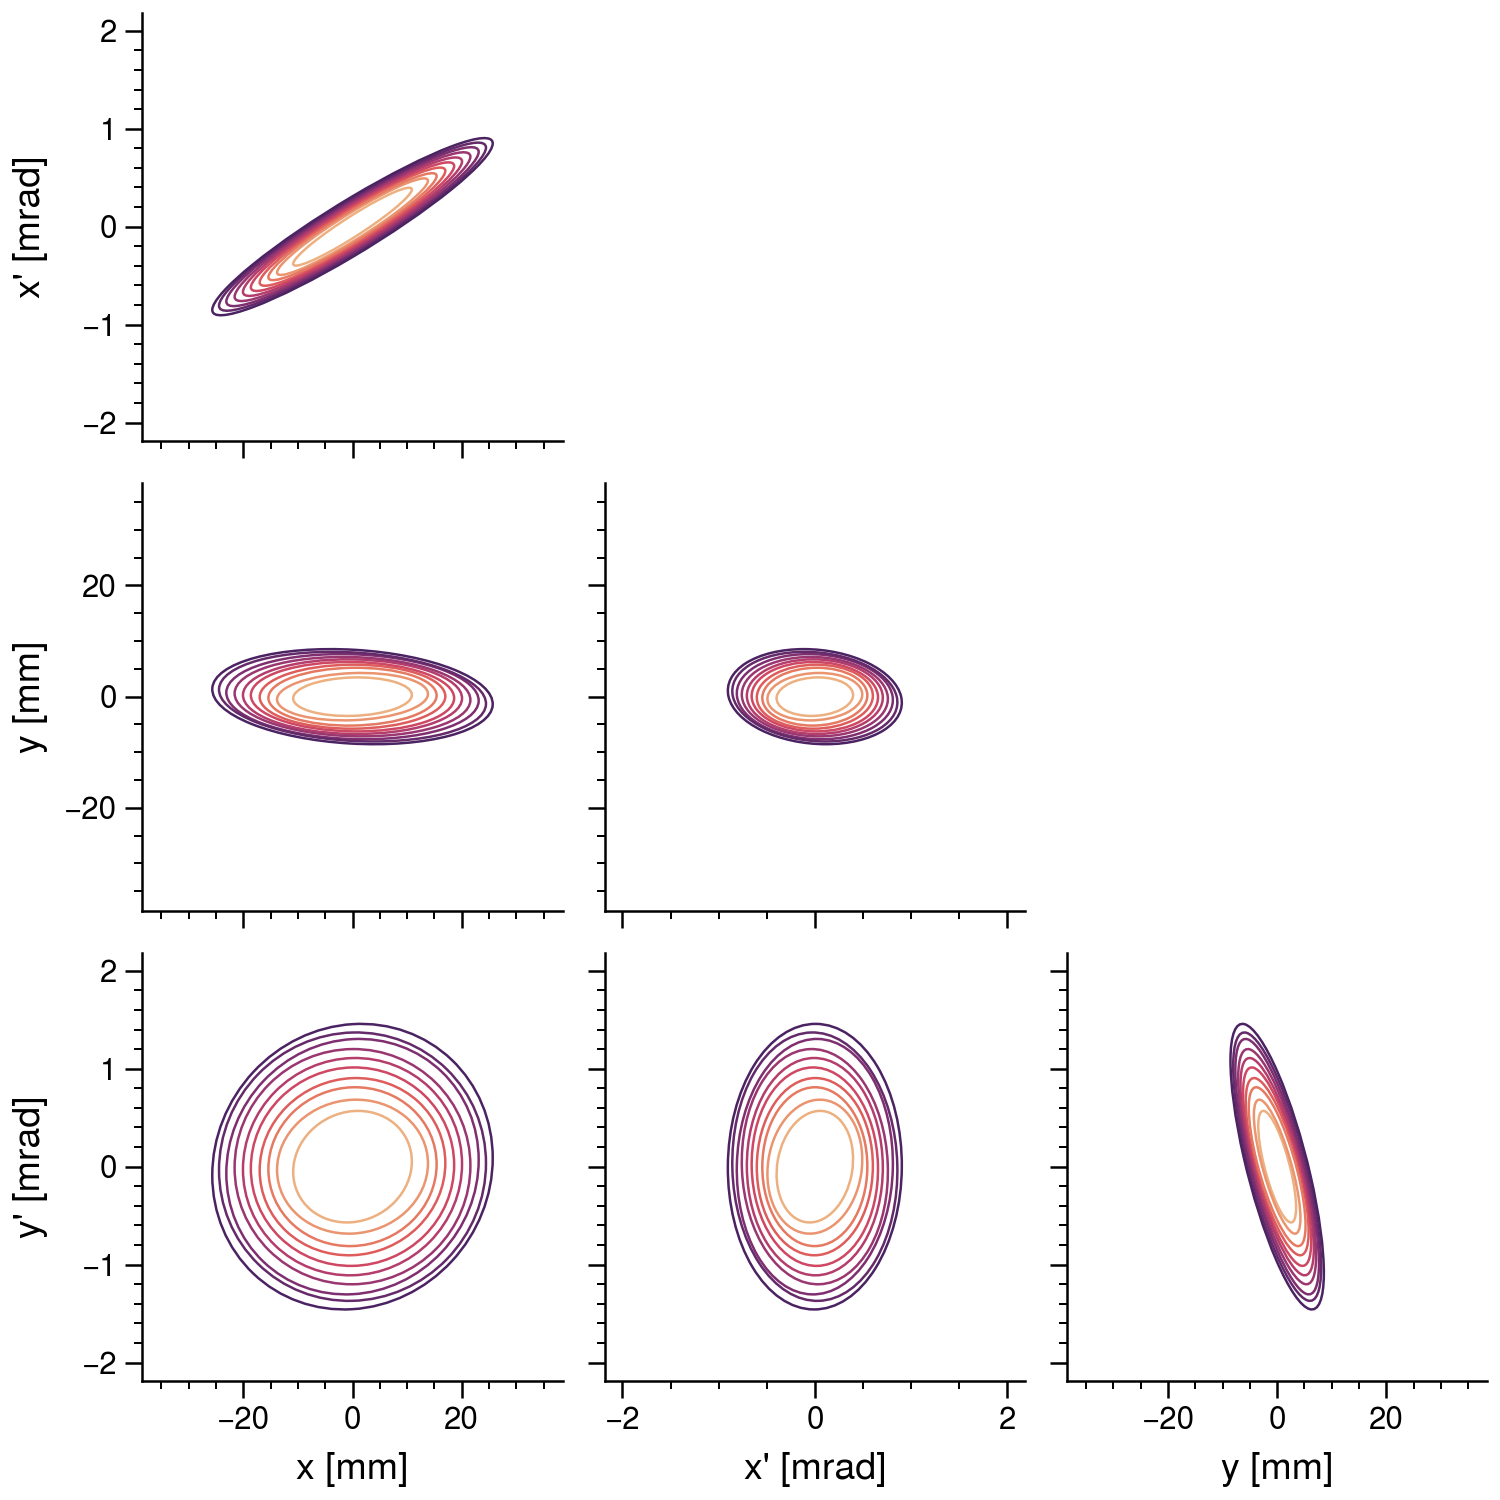
\includegraphics[width=\textwidth]{Images/chapter5/exp2/corner.png}
    \end{subfigure}
    \hfill
    \begin{subfigure}[t]{0.39\textwidth}
        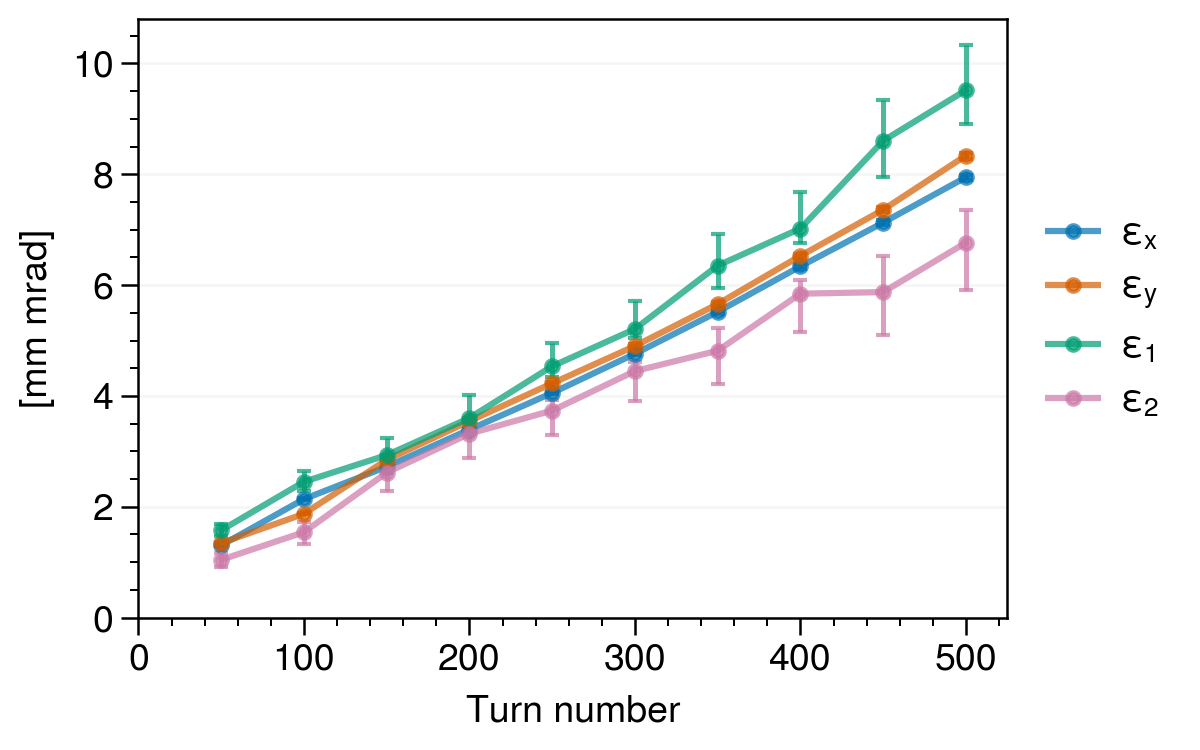
\includegraphics[width=\textwidth]{Images/chapter5/exp2/emittances.png}
    \end{subfigure}
    \caption{Reconstructed emittances and covariance ellipses from Experiment 2.}
    \label{fig:exp2_emittances}
\end{figure}
%
The apparent emittances grow linearly from a small value, as intended. The measured apparent emittances are equal throughout injection, which is not expected from Eq.~\ref{eq:painted_emittance_ratio}. A possible explanation is that the beam experienced space-charge-driven emittance exchange as it circulated, resulting in equal emittances as new particles were added to the distribution (see Chapter \ref{chap-2}). 

The reconstructed intrinsic emittances begin to diverge at the end of injection, but the measured cross-plane correlation is small. Additionally, the error bars are larger than in the previous experiment; this is most likely due to a larger mismatch of the beam Twiss parameters at the RTBT entrance, which is expected given the increase in beam perveance at 0.8 GeV energy and reduced beam size. Possible bias in the measurement, expected to be near the 10\% level, must also be kept in mind. Given the small measured cross-plane correlation and larger error bars, it cannot be claimed that the 4D emittance is significantly reduced. 

A simulation of this case is shown in Fig.~\ref{fig:exp2_sim}.
%
\begin{figure}[!p]
    \centering
    \begin{subfigure}{\textwidth}
        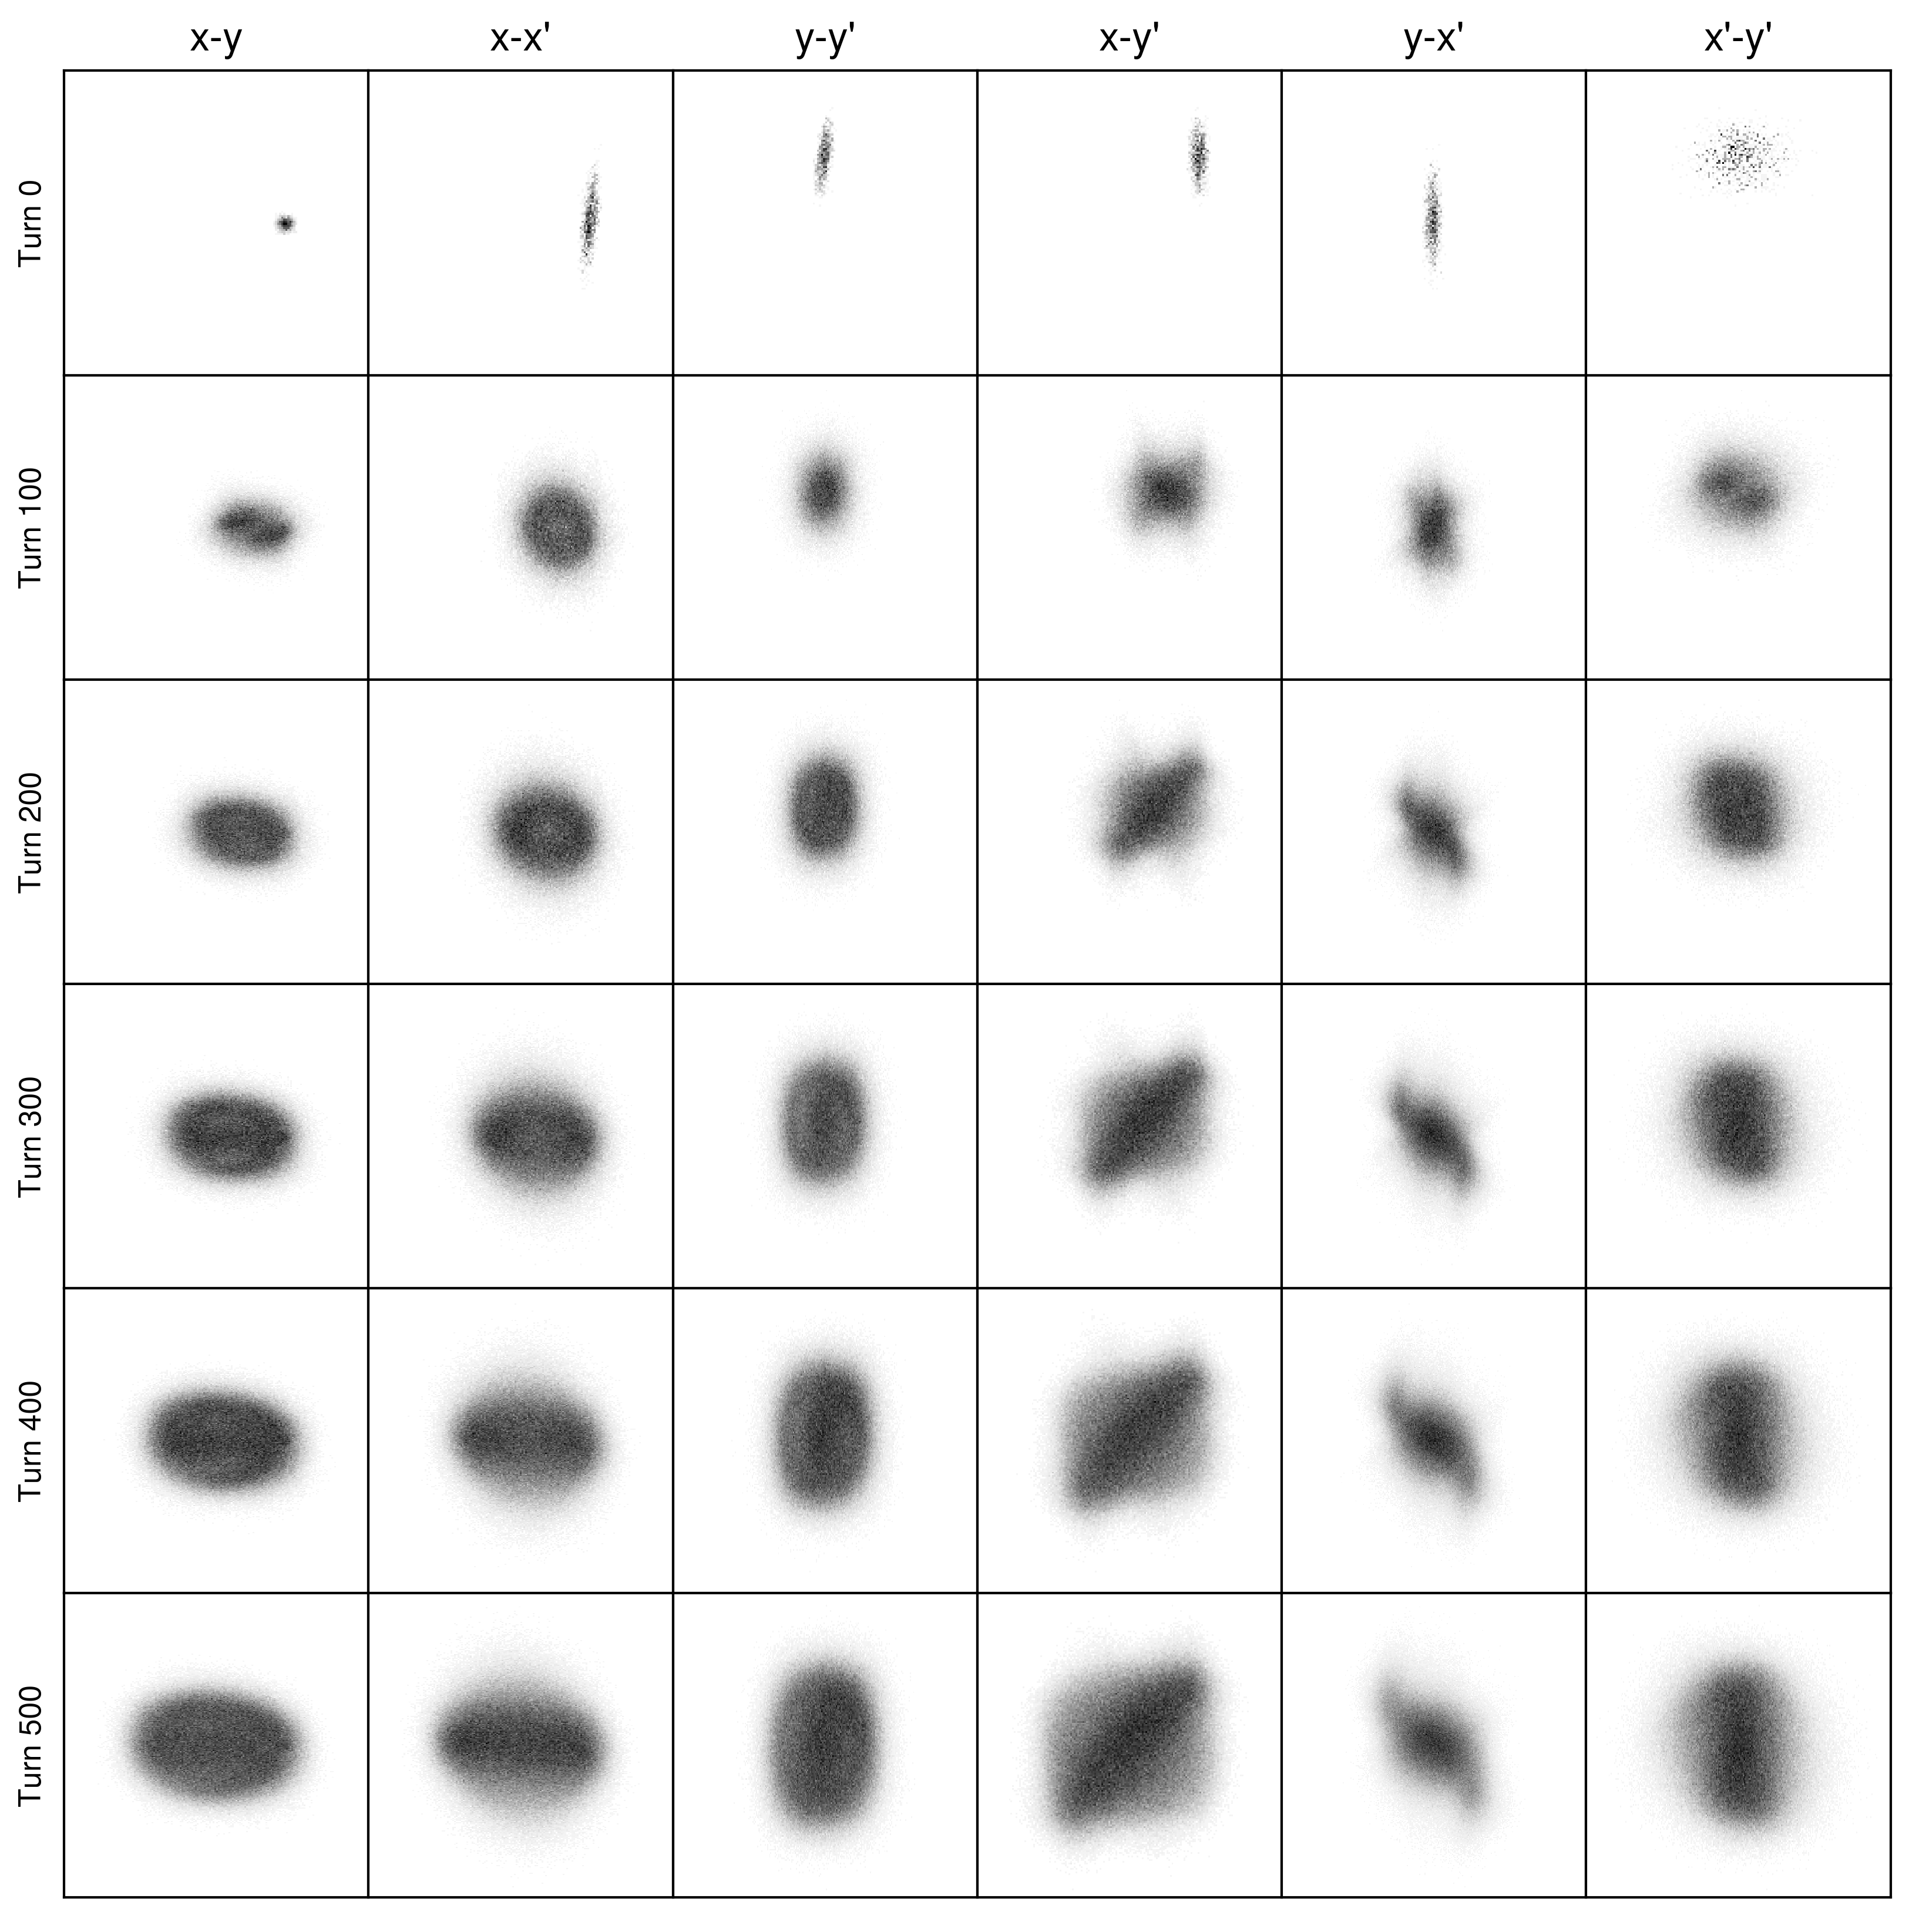
\includegraphics[width=\textwidth]{Images/chapter5/exp2/sim_snapshots.png}
    \end{subfigure}
    \vfill
    \vspace*{1.0cm}
    \vfill
    \begin{subfigure}{0.7\textwidth}
        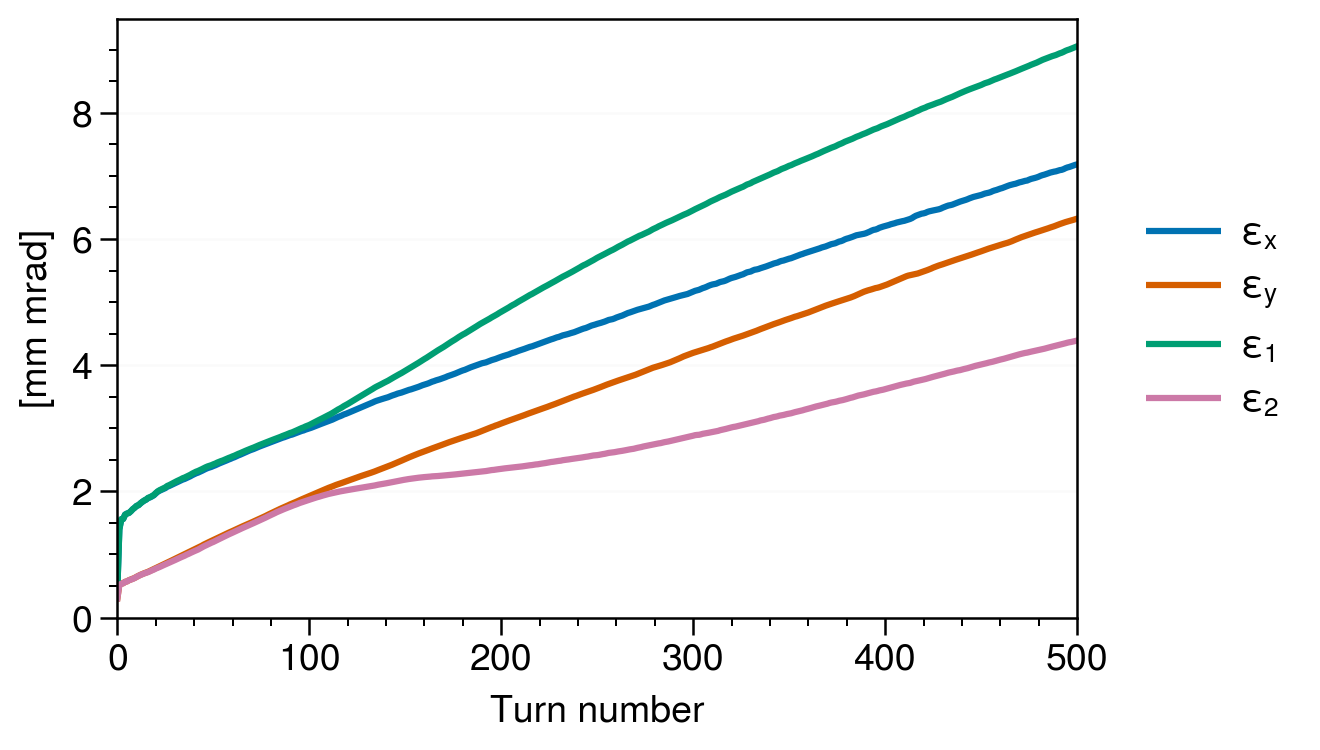
\includegraphics[width=\textwidth]{Images/chapter5/exp2/sim_emittances.png}
    \end{subfigure}
    \caption{Simulation of Experiment 2.}
    \label{fig:exp2_sim}
\end{figure}
%
Notice that $\varepsilon_2$ begins to flatten after turn 100, but does not remain flat, and although the final $x$-$y'$ projection has a higher density along the painting path, the linear correlation is significantly blurred. Space charge has a strong effect on the evolution at this intensity, energy, and beam size, providing some explanation for the measurements in Fig.~\ref{fig:exp2_emittances}.



\section{Experiment 3}

The goal of this final experiment was to vary the free parameters of the machine and record the intrinsic emittances in each case, with the plan to examine the most promising case in more detail. To begin, the setup from Experiment 2 was repeated. One difference was that the bunch length was increased from roughly 30/64 of the ring length to 40/64 of the ring length to better approximate a coasting beam. This was done by modifying the chopper settings before the linac and should have increased the total charge of the bunch without changing its charge density. Beam current monitor (BMC) measurements of the longitudinal distribution in the ring are shown in Fig.~\ref{fig:bcm_waterfall}; it is clear that there are no strong peaks from RF bunching.
%
\begin{figure}[!p]
    \centering
    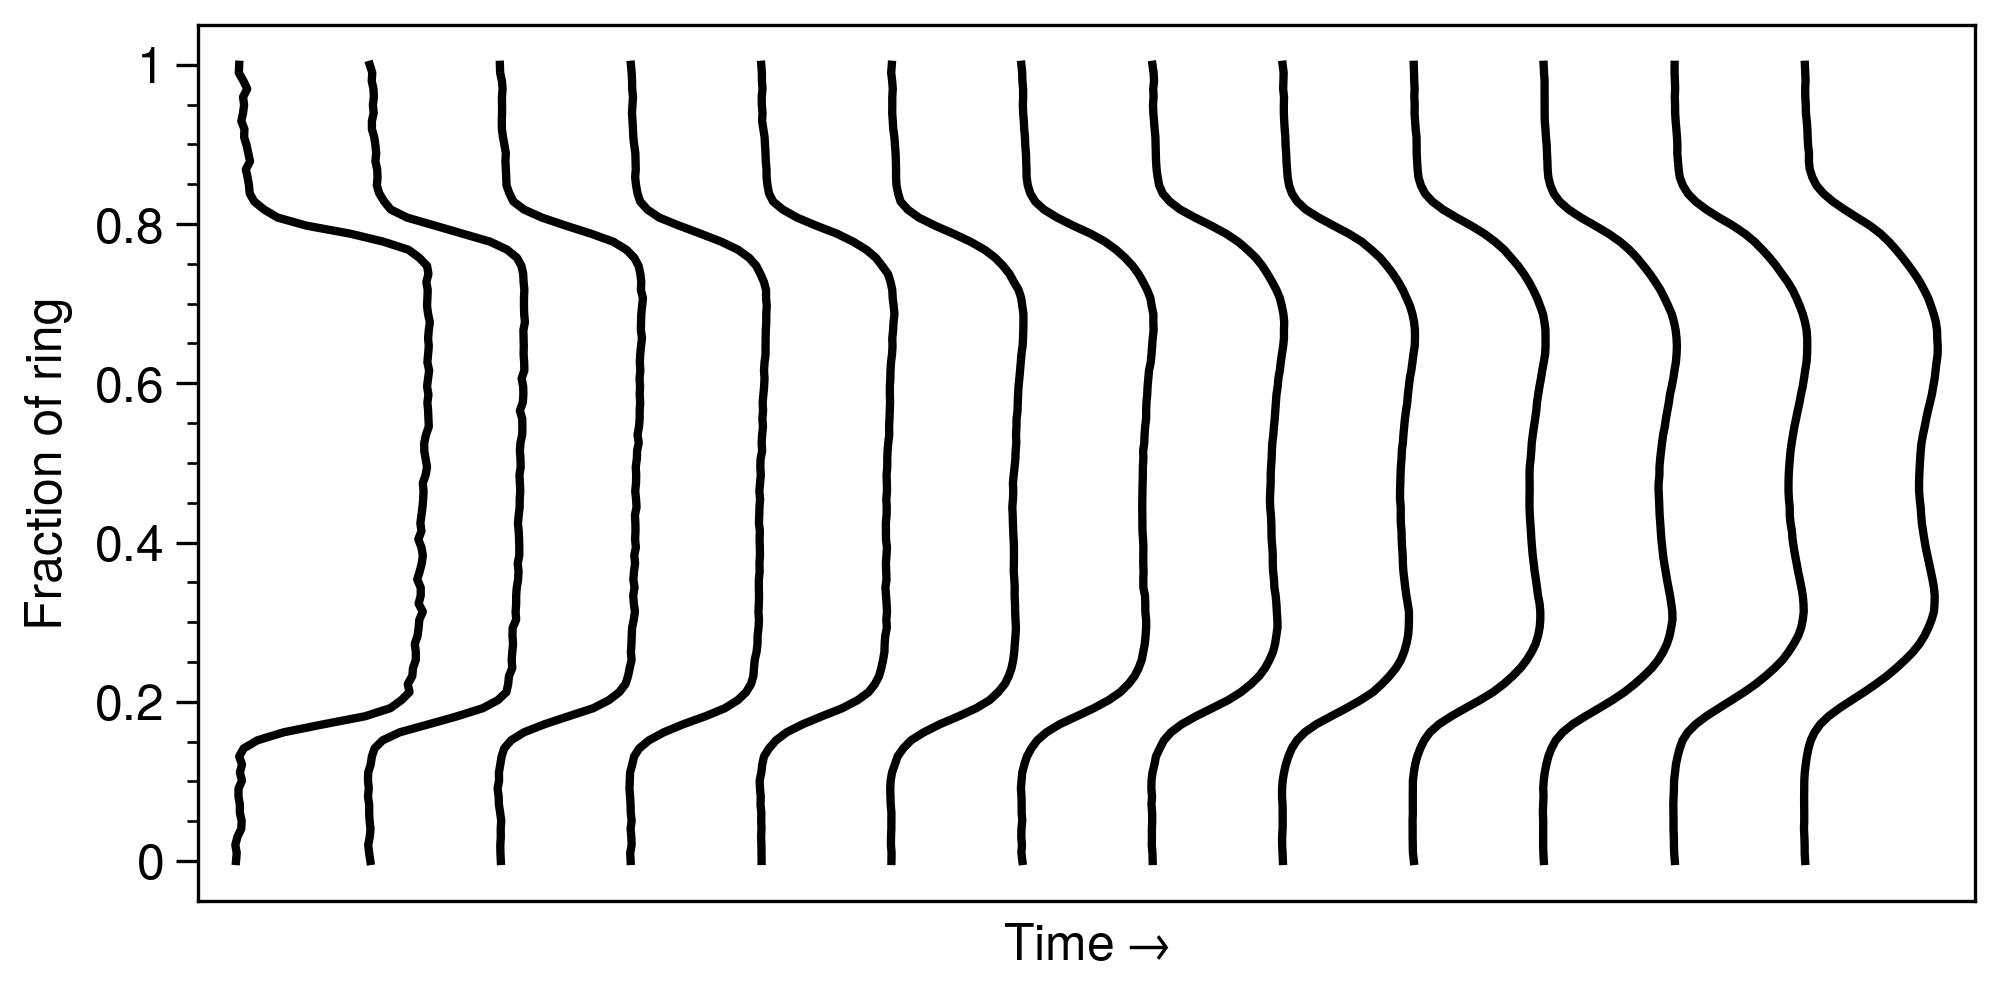
\includegraphics[width=\textwidth]{Images/chapter5/exp3/bcm_waterfall.png}
    \caption{Evolution of the longitudinal distribution in the ring as measured by a beam current monitor (BCM).}
    \label{fig:bcm_waterfall}
\end{figure}
%

Since the vertical injection angle could not be increased, the remaining free parameters were the beam intensity and horizontal beam size: measured emittances for three different intensities and two different painting settings are shown in Fig.~\ref{fig:exp3_search}.\footnote{The intensities are not exact; they are obtained by multiplying the nominal minipulse intensity by the number of injected turns.} Collective effects seem to affect the final distribution. It is somewhat surprising that the split in the intrinsic emittances increased with the beam intensity. 
%
\begin{figure}[!p]
    \centering
    \vspace*{1.0cm}
    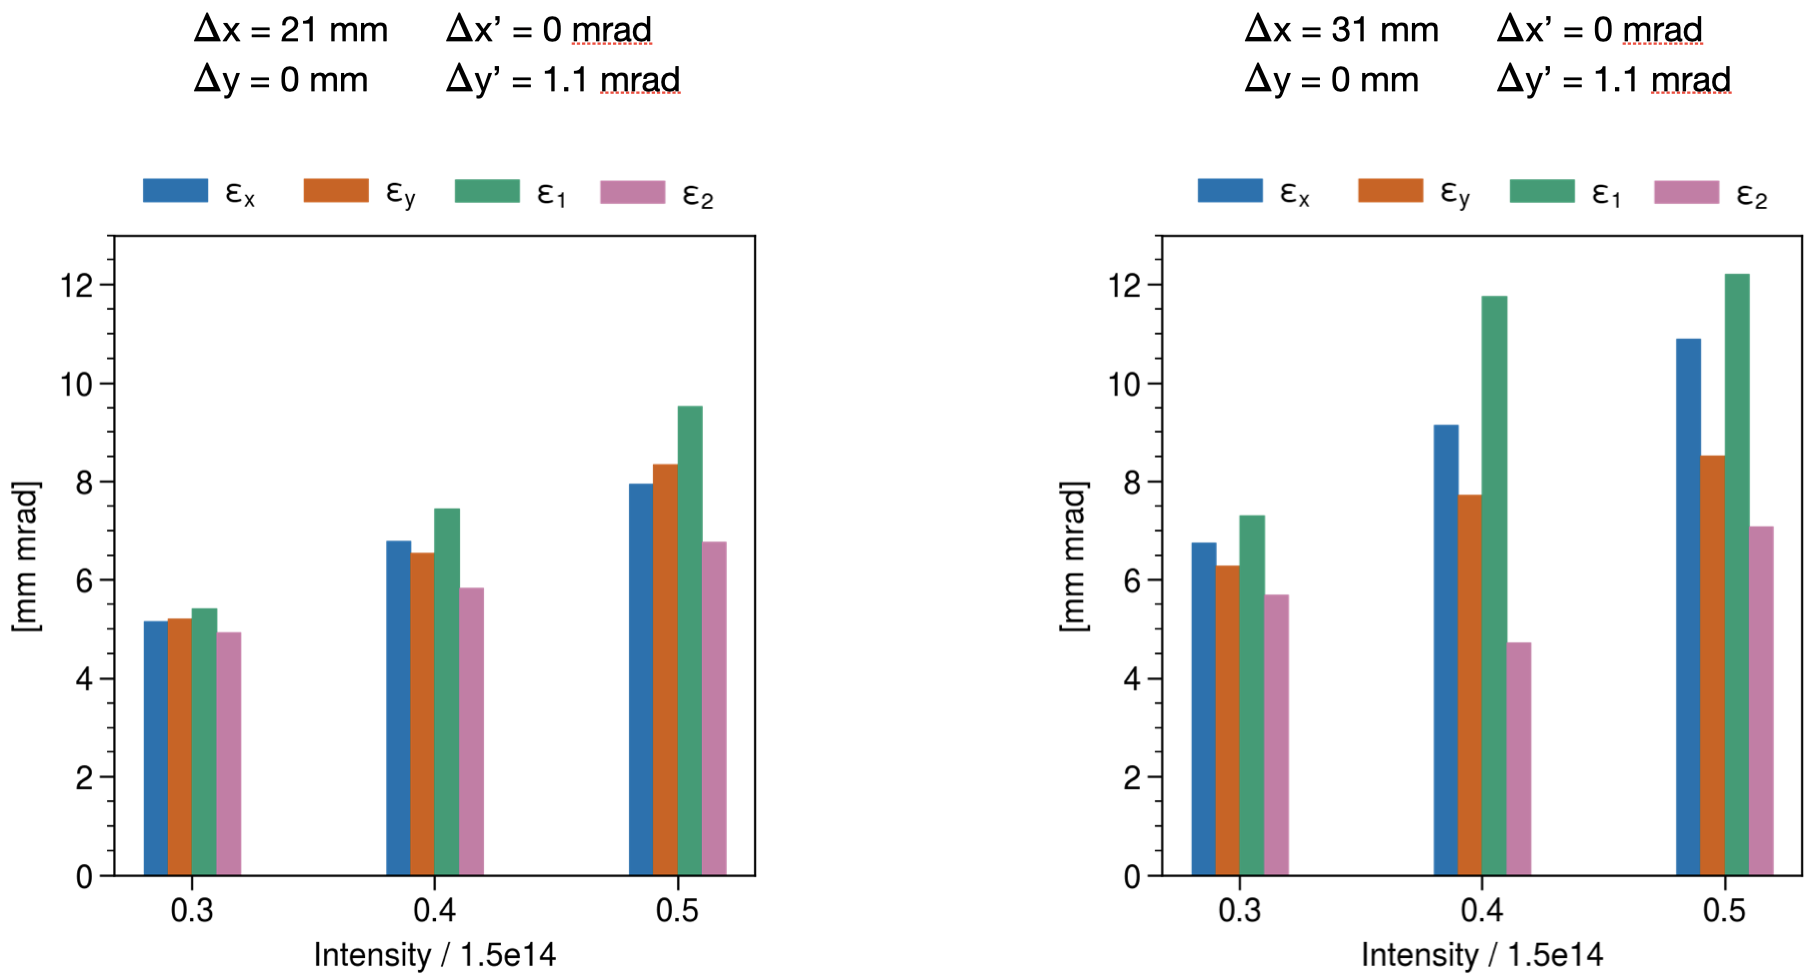
\includegraphics[width=\textwidth]{Images/chapter5/exp3/search.png}
    \caption{Measured emittances vs. beam intensity for two sets of injected coordinates. (Error bars not shown).}
    \label{fig:exp3_search}
    \vspace*{1.0cm}
\end{figure}
%
The measurement process of the previous two experiments was repeated for the center cluster in the right subplot: which amounts to a 50\% increase in horizontal beam size and 20\% reduction in beam size. 

The measured wire-scanner profiles are shown in Fig.~\ref{fig:exp3_wsmeas}.
%
\begin{figure}[!p]
    \centering
    \begin{subfigure}{\textwidth}
        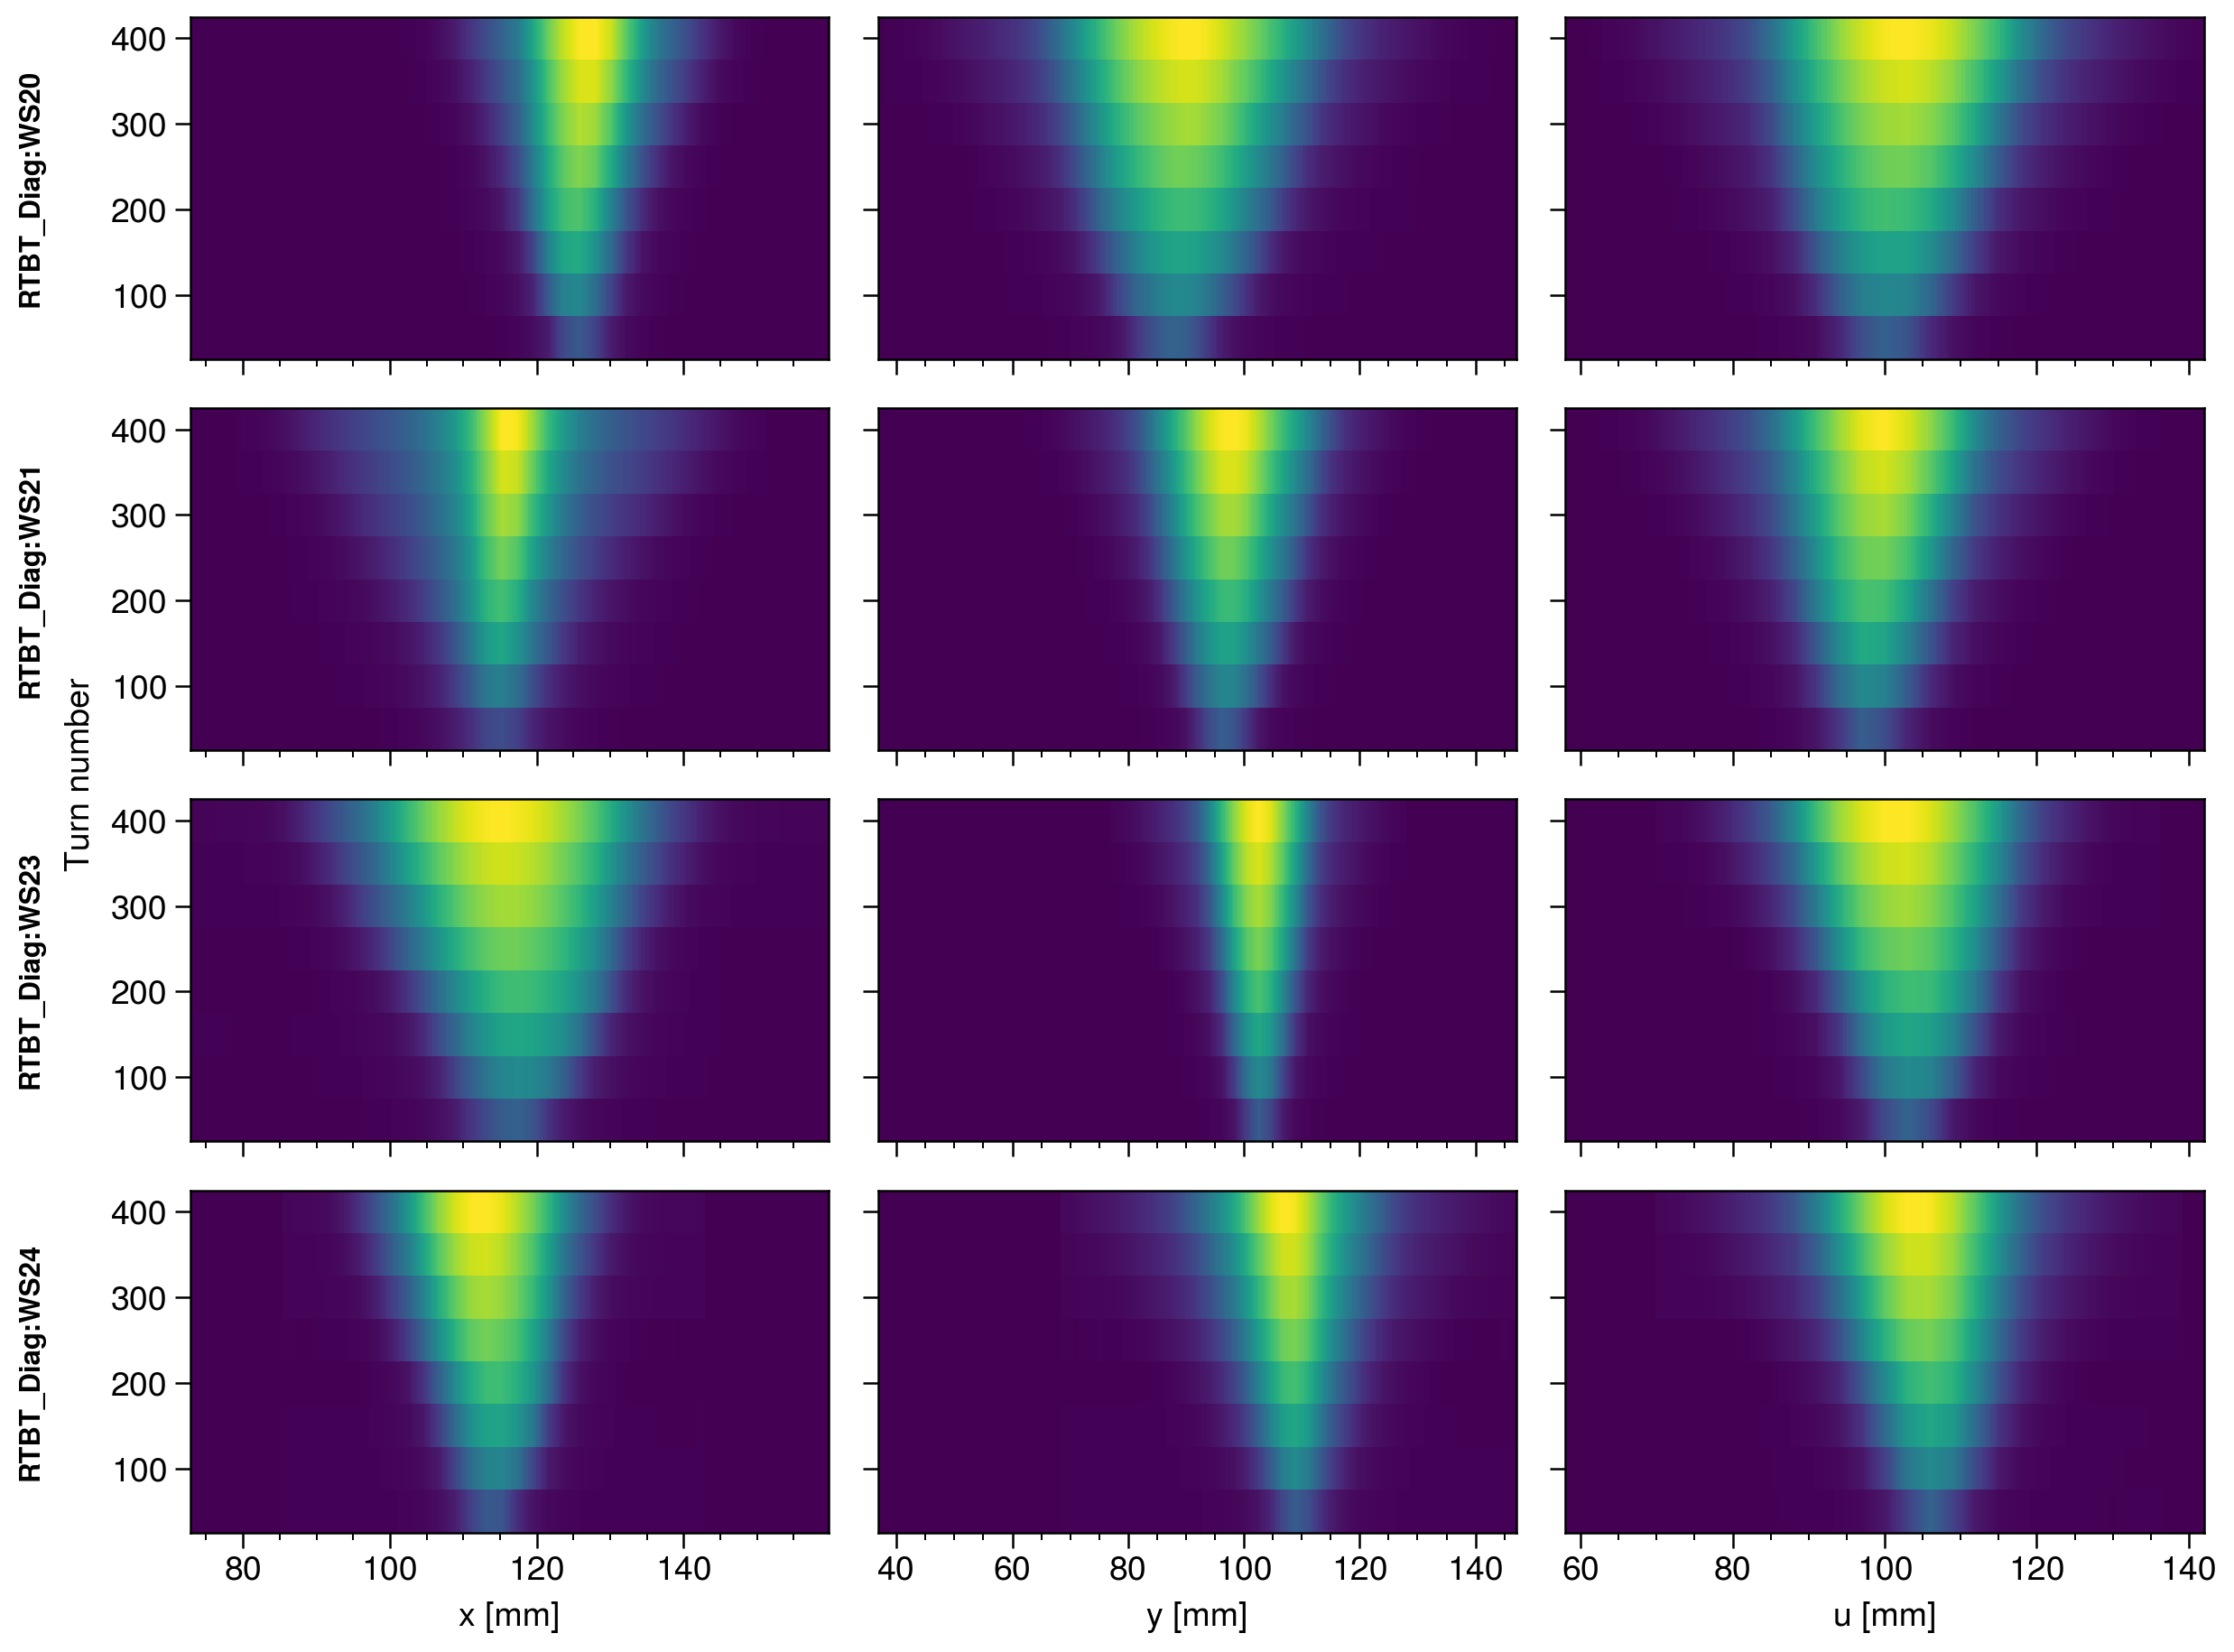
\includegraphics[width=\textwidth]{Images/chapter5/exp3/waterfall.png}
    \end{subfigure}
    \vfill
    \vspace*{1.25cm}
    \vfill
    \begin{subfigure}{\textwidth}
        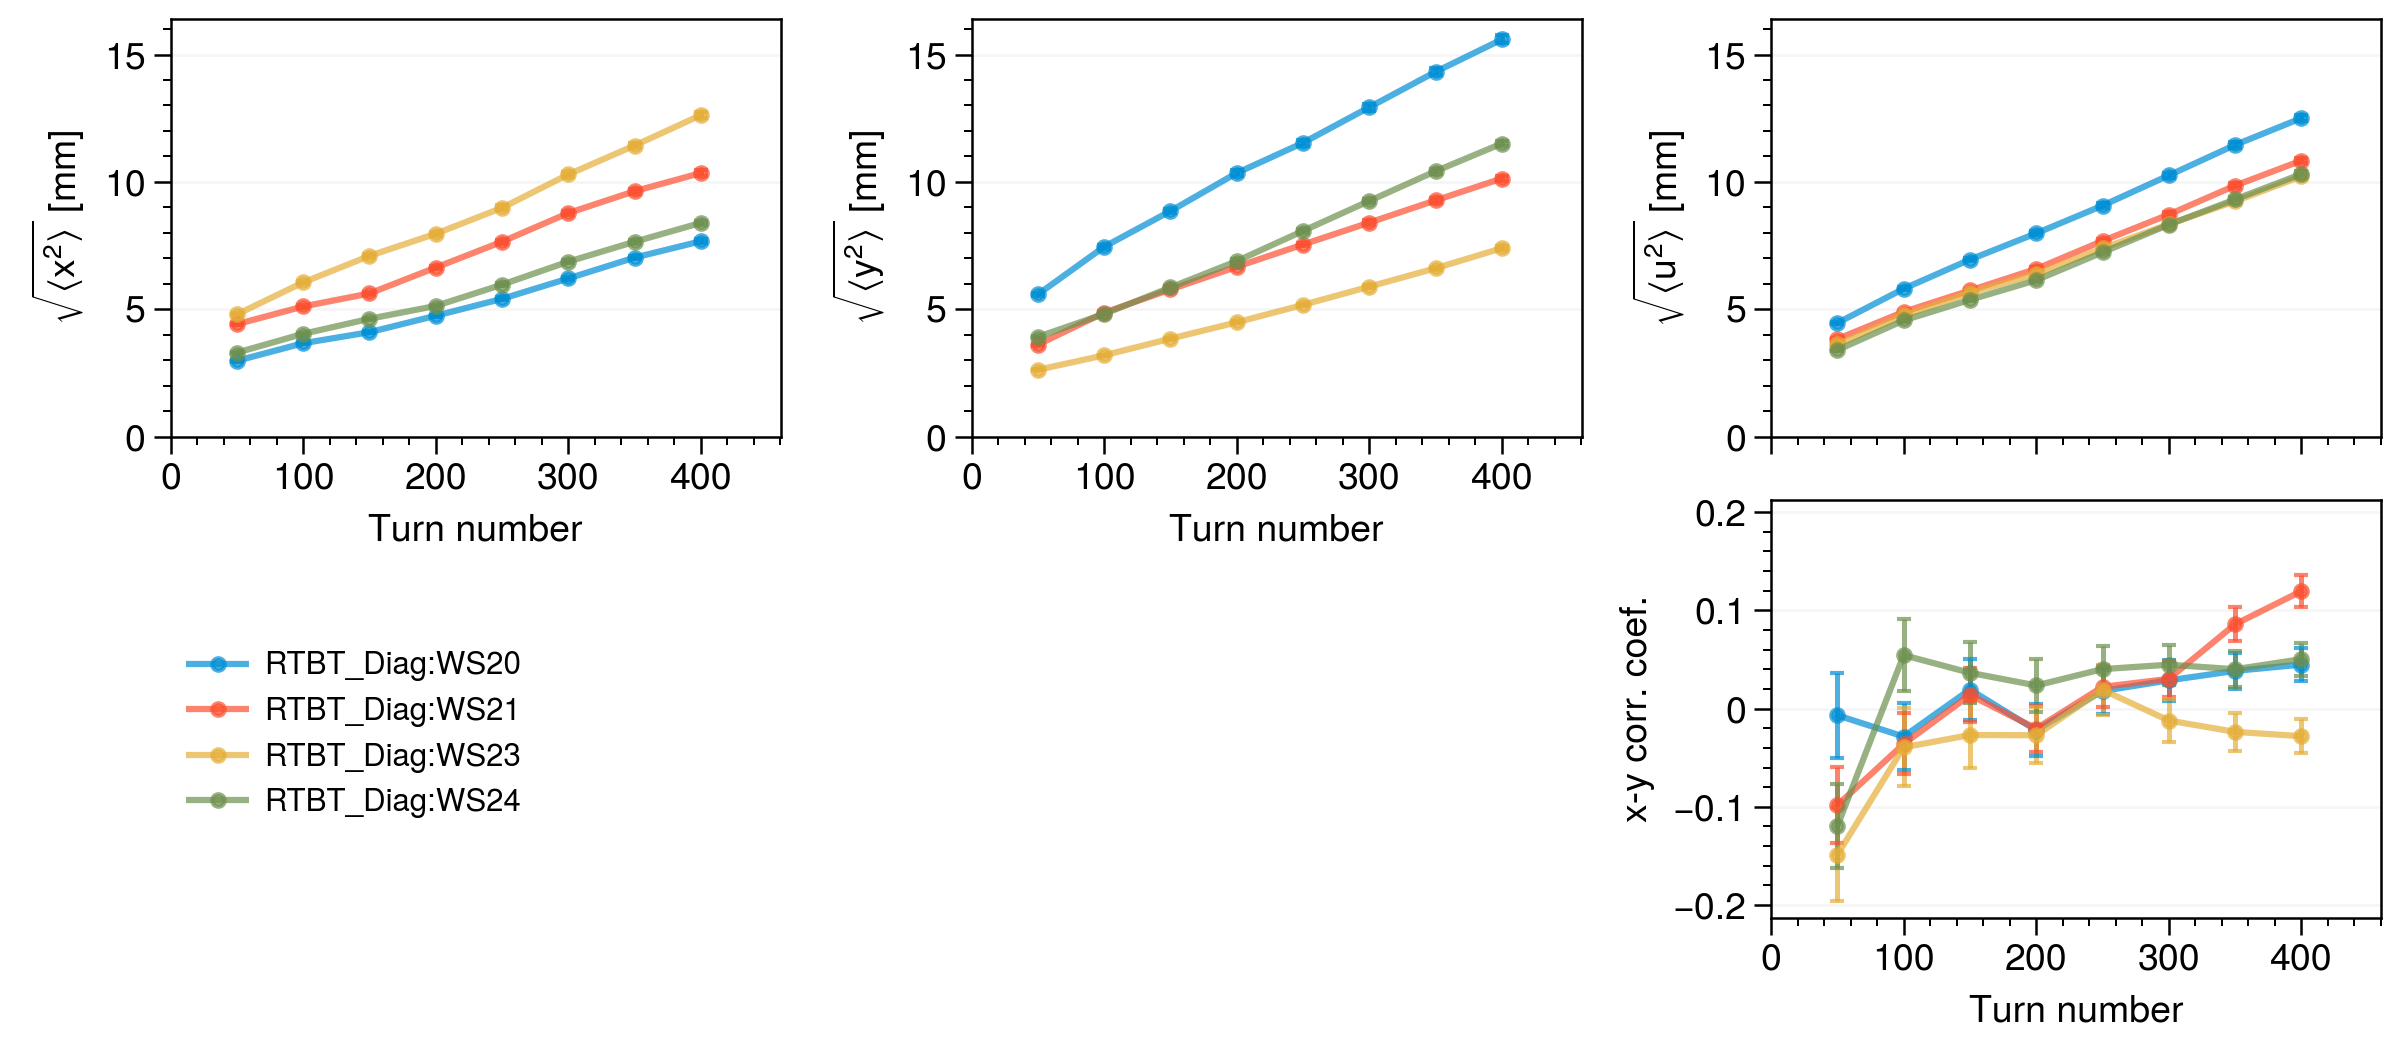
\includegraphics[width=\textwidth]{Images/chapter5/exp3/rms.png}
    \end{subfigure}
    \caption{Measured wire-scanner profiles from Experiment 3.}
    \label{fig:exp3_wsmeas}
\end{figure}
%
The beam size curves do not fit the square root dependence as well as in Experiment 2. The measured profiles look similar to those in Experiment 2, although the horizontal projection at WS21 has developed a sharp peak surrounded by a lower density cloud. 

Fig.~\ref{fig:exp3_emittances} shows the reconstructed emittances and covariance ellipses.
%
\begin{figure}[!p]
    \centering
    \begin{subfigure}{0.6\textwidth}
        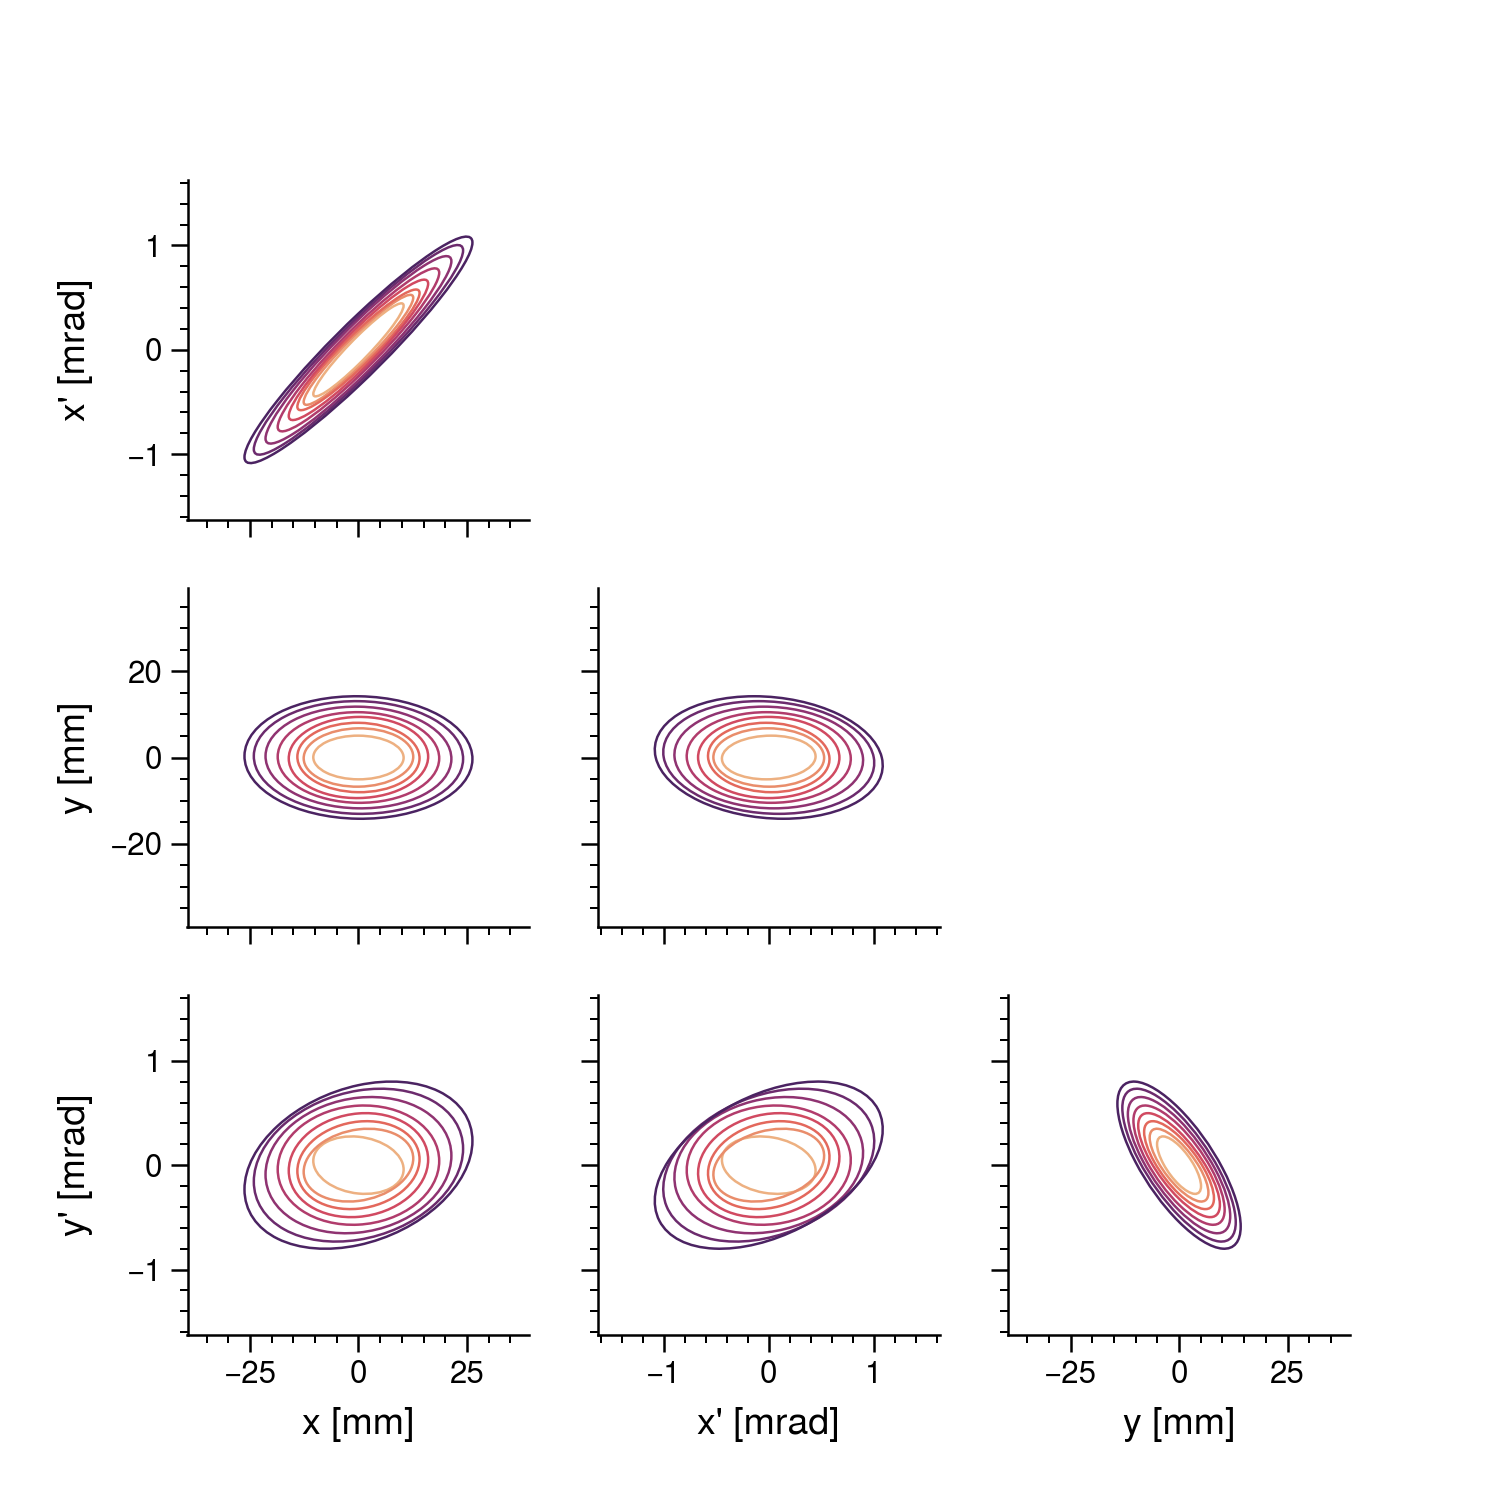
\includegraphics[width=\textwidth]{Images/chapter5/exp3/corner.png}
    \end{subfigure}
    \hfill
    \begin{subfigure}[t]{0.39\textwidth}
        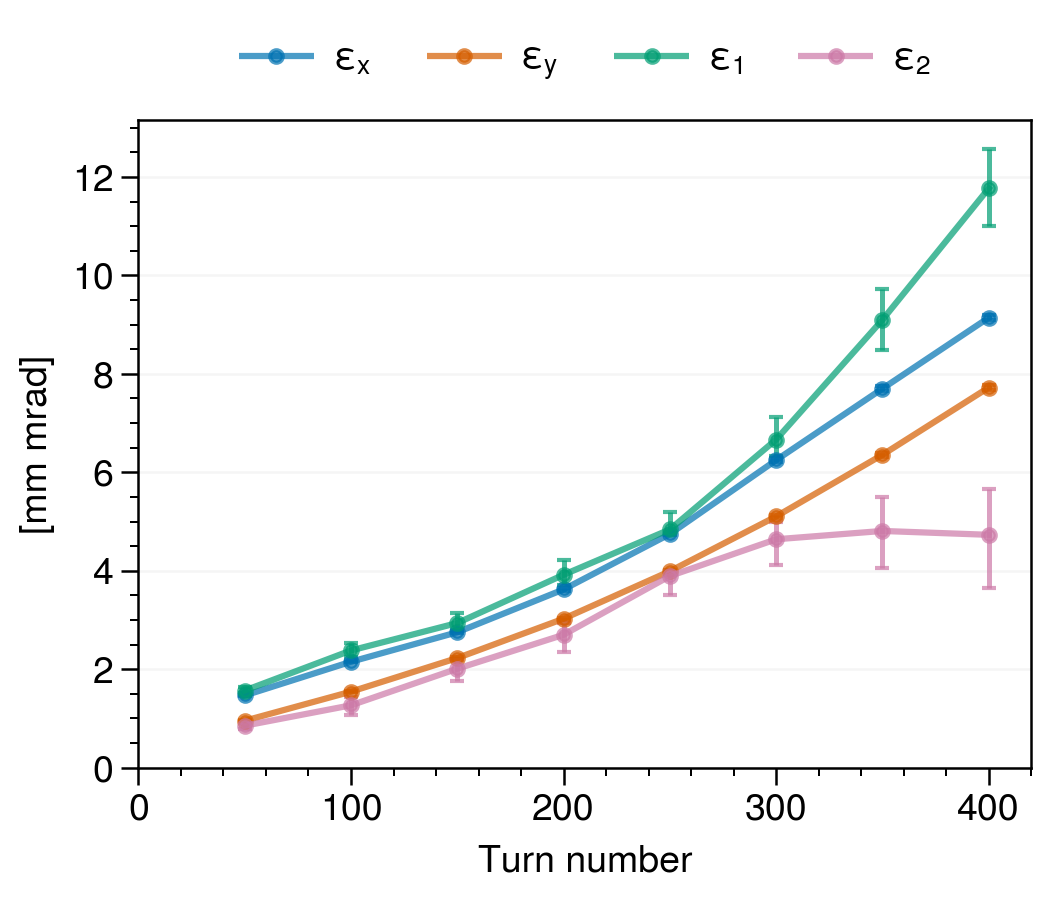
\includegraphics[width=\textwidth]{Images/chapter5/exp3/emittances.png}
    \end{subfigure}
    \caption{Reconstructed emittances and covariance ellipses from Experiment 3.}
    \label{fig:exp3_emittances}
\end{figure}
% 
From Eq.~\ref{eq:painted_emittance_ratio}, the ratio $\varepsilon_y / \varepsilon_x$ is expected to be quite small — around 1/8 — but again, the apparent emittances remain nearly equal. A future study could split the tunes and perform correlated painting with zero offset from the foil, varying $x_{max}$, and $y_{max}$ to examine whether this phenomenon is caused by coupled space charge forces.

Although the error bars remain large, the reconstructed $\varepsilon_{1,2}$ significantly deviate from $\varepsilon_{x,y}$ after 300 turns, which manifests in the tilting of the reconstructed ellipses in the cross-plane projections. This was the largest correlation measured so far. Beam images on the target were also collected as the horizontal and vertical phase advances were scanned. The bunch length was inadvertently decreased by a factor of three beforehand, precluding direct comparison with the wire-scanner measurements. Two of the images are shown in Fig.~\ref{fig:exp3_target_scan}. 
%
\begin{figure}[!p]
    \centering
    \vspace*{5cm}
    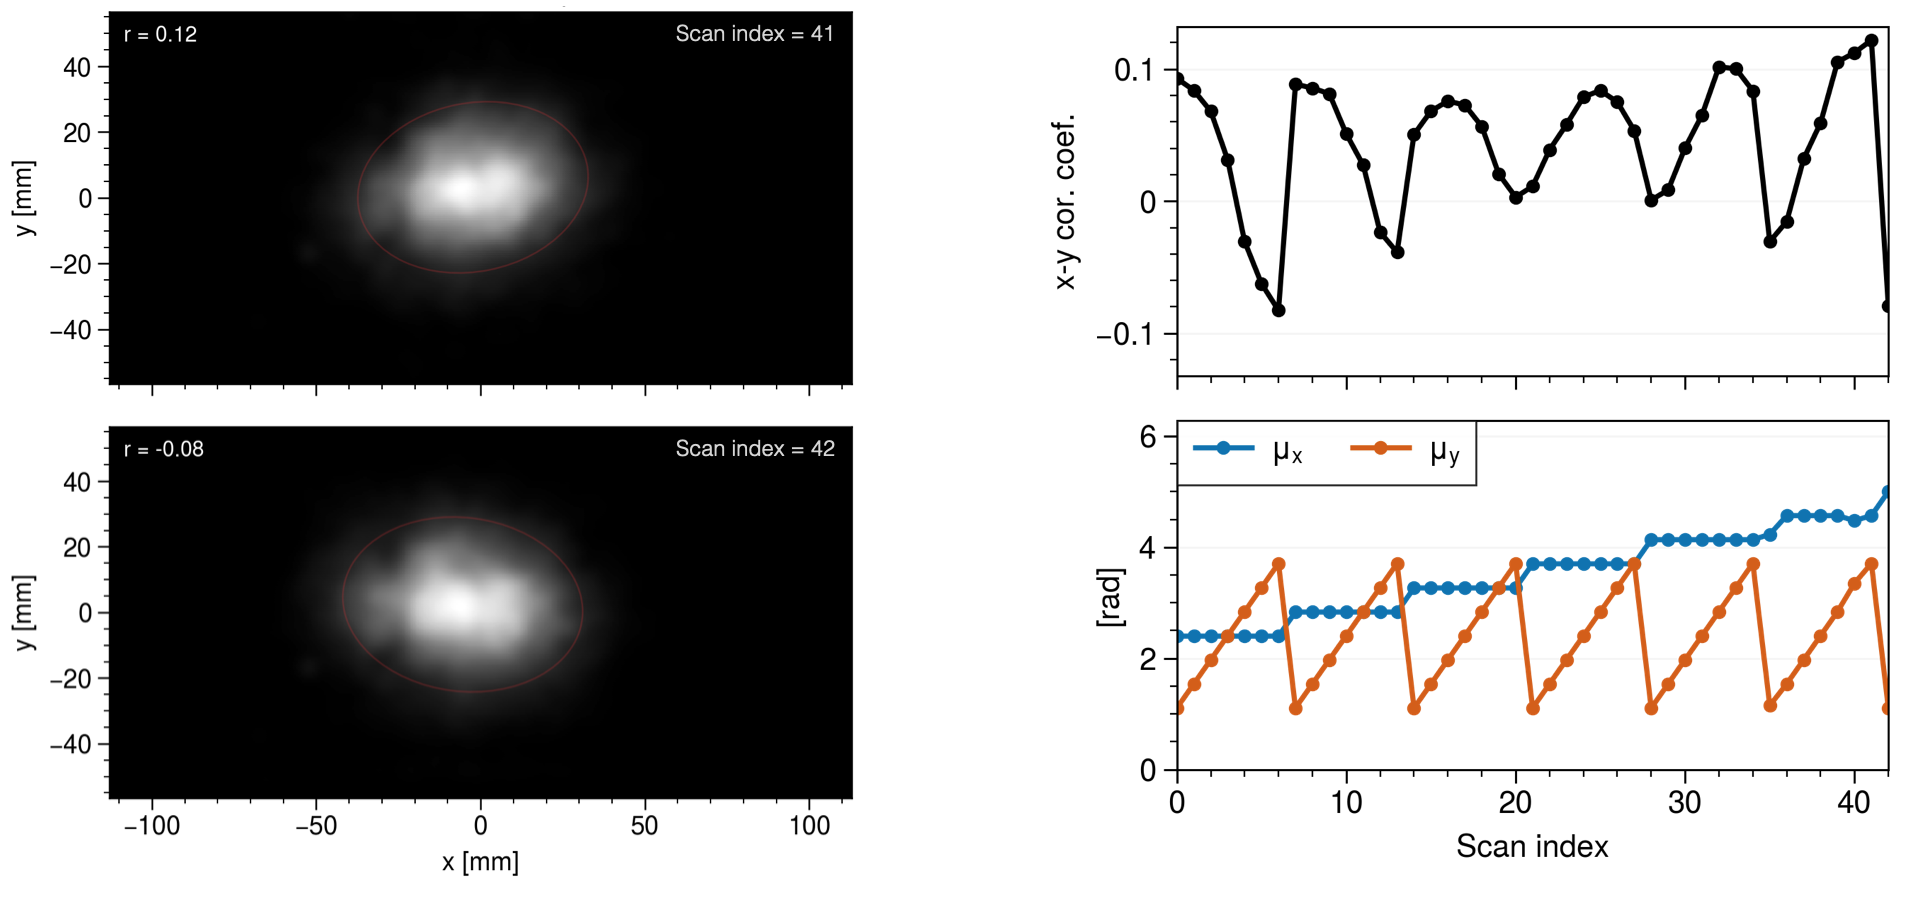
\includegraphics[width=\textwidth]{Images/chapter5/exp3/target_scan/target_scan.png}
    \caption{Scan of the phase advances at the target. Left: processed images on last two steps in the scan. Top right: $x$-$y$ correlation coefficients computed from the images. Bottom right: Phase advances at the target.}
    \label{fig:exp3_target_scan}
    \vspace*{5cm}
\end{figure}
%
The $x$-$y$ correlation coefficient, although small, clearly depends on the phase advances, demonstrating that there were cross-plane correlations in the beam.\footnote{The $x$-$y$ correlation coefficient is calculated directly from the image.}

It is recommended that this setup be repeated in a future experiment. It should be examined whether additional slight changes to the RTBT optics can reduce the uncertainty in the fixed-optics measurement, and the multi-optics measurement should be performed on the final distribution for comparison. Additionally, images of the same beam should be collected as the phase advances are scanned at the target.

We conclude with a simulation of this experiment in Fig.~\ref{fig:exp3_sim}.
%
\begin{figure}[!p]
    \centering
    \begin{subfigure}{\textwidth}
        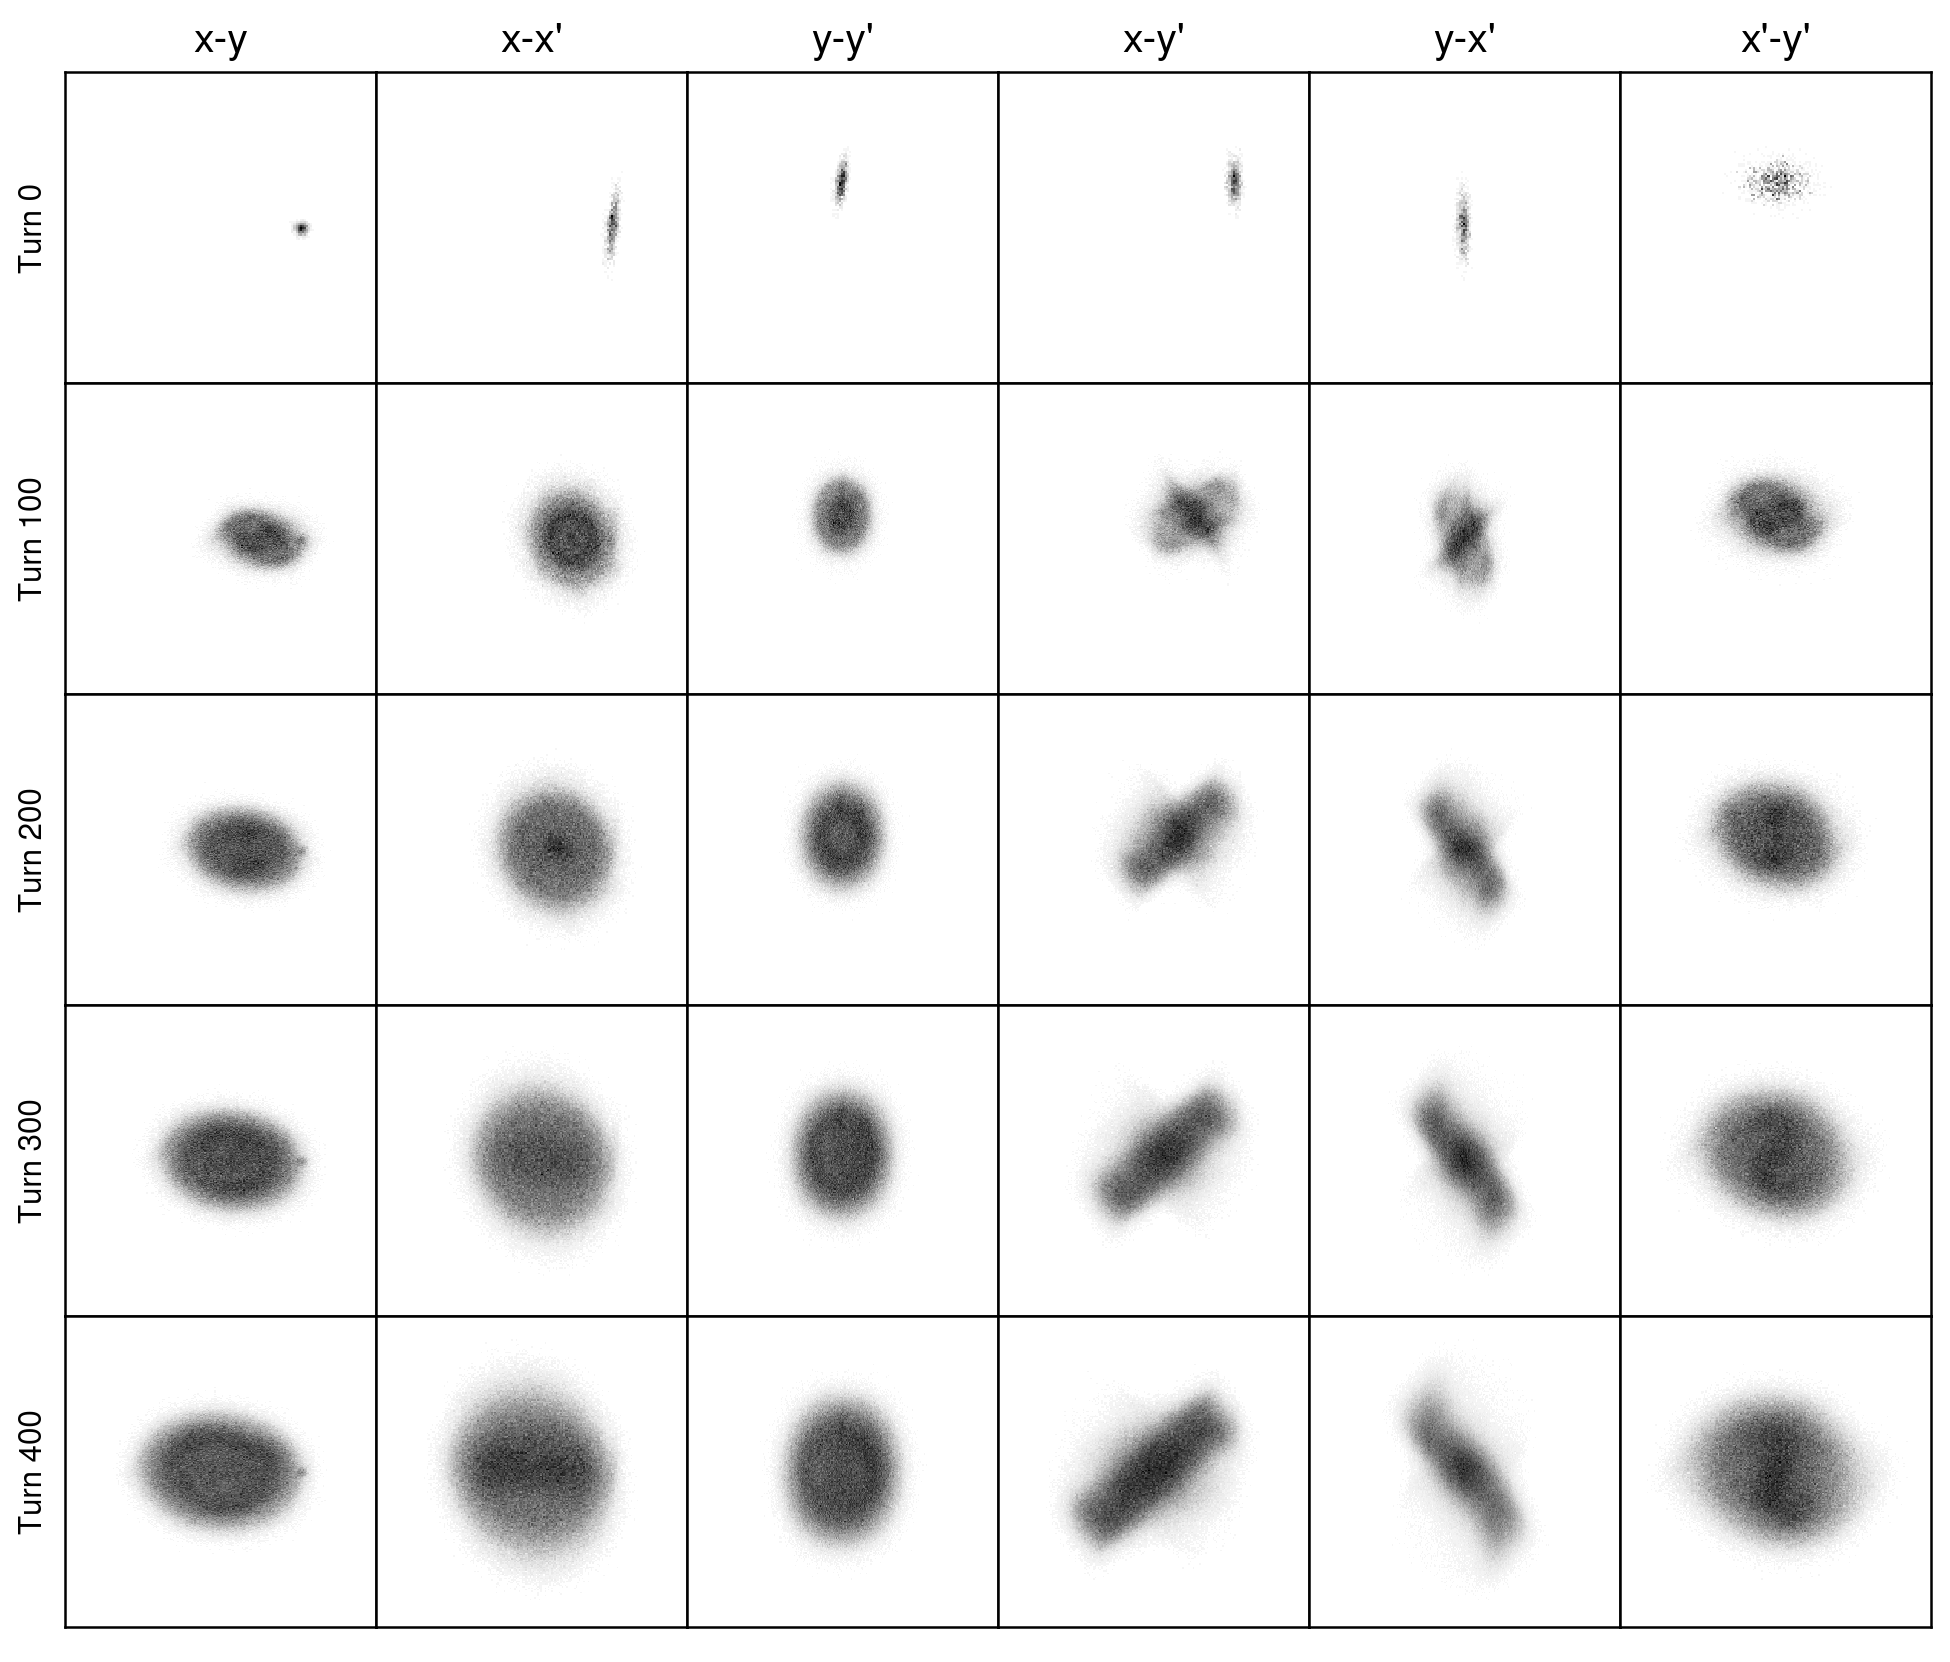
\includegraphics[width=\textwidth]{Images/chapter5/exp3/sim_snapshots.png}
    \end{subfigure}
    \vfill
    \vspace*{1.0cm}
    \vfill
    \begin{subfigure}{0.7\textwidth}
        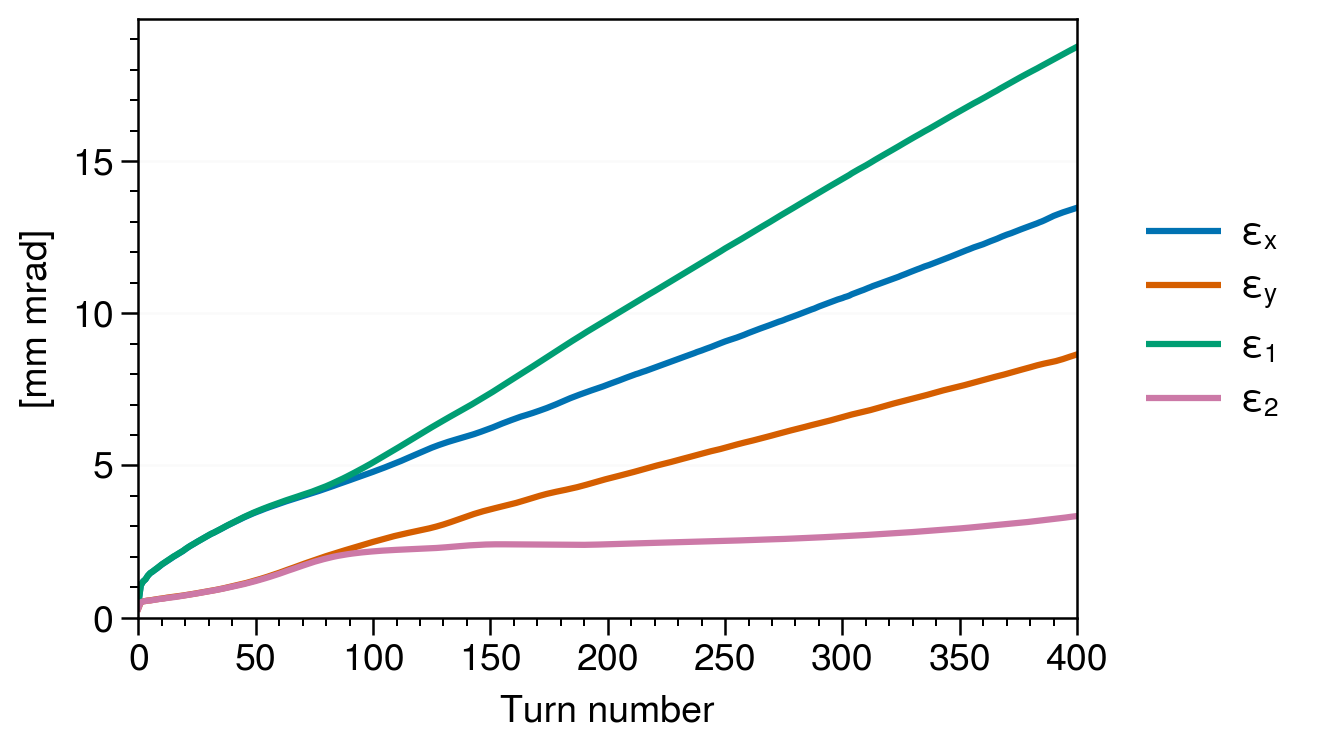
\includegraphics[width=\textwidth]{Images/chapter5/exp3/sim_emittances.png}
    \end{subfigure}
    \caption{Simulation of Experiment 3.}
    \label{fig:exp3_sim}
\end{figure}
%
This looks closer to the best-case scenario from Chapter \ref{chap-3}, even though solenoids are not present in the ring and the vertical injection angle is limited. Again, the predicted ratio $\varepsilon_1 / \varepsilon_2$ is larger than what was measured. We repeated the simulation as the horizontal tune was varied in steps of 0.005 around its original value of 6.18. At $\nu_x = 6.2$, all cross-plane correlation in the beam was eliminated. Fig.~\ref{fig:exp3_sim_nux6.195_nuy6.18} shows the case when $\nu_x = 6.195$. 
%
\begin{figure}[!p]
    \centering
    \begin{subfigure}{\textwidth}
        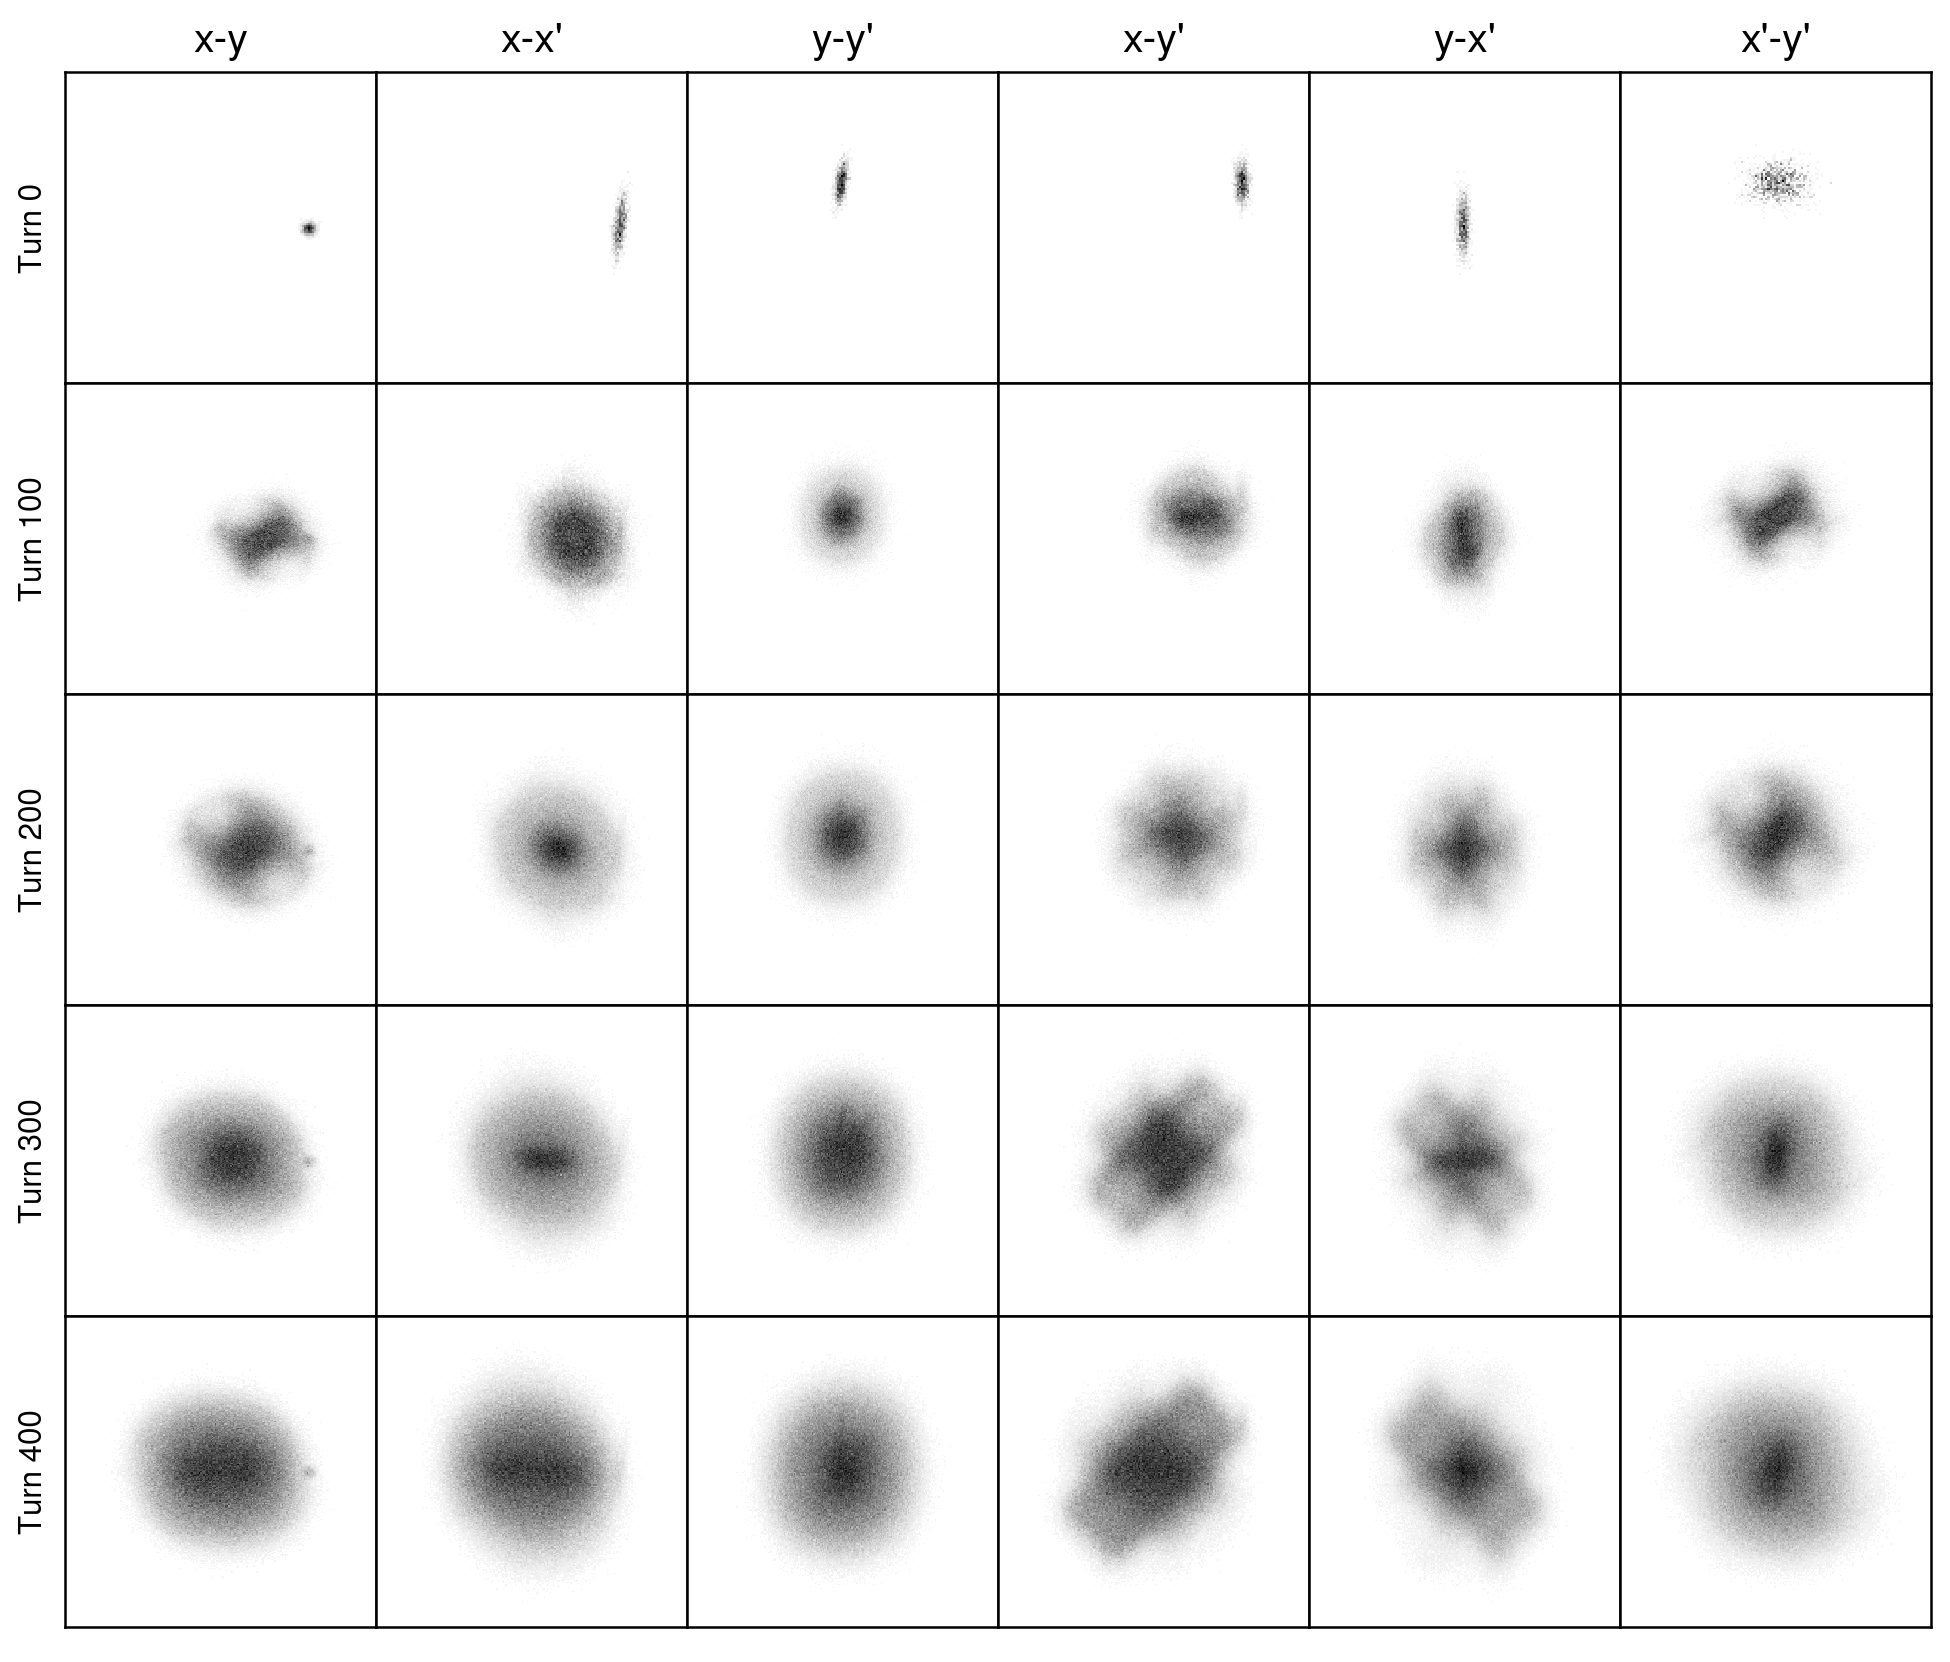
\includegraphics[width=\textwidth]{Images/chapter5/exp3/sim_snapshots_nux6.195_nuy6.18.png}
    \end{subfigure}
    \vfill
    \vspace*{1.0cm}
    \vfill
    \begin{subfigure}{0.7\textwidth}
        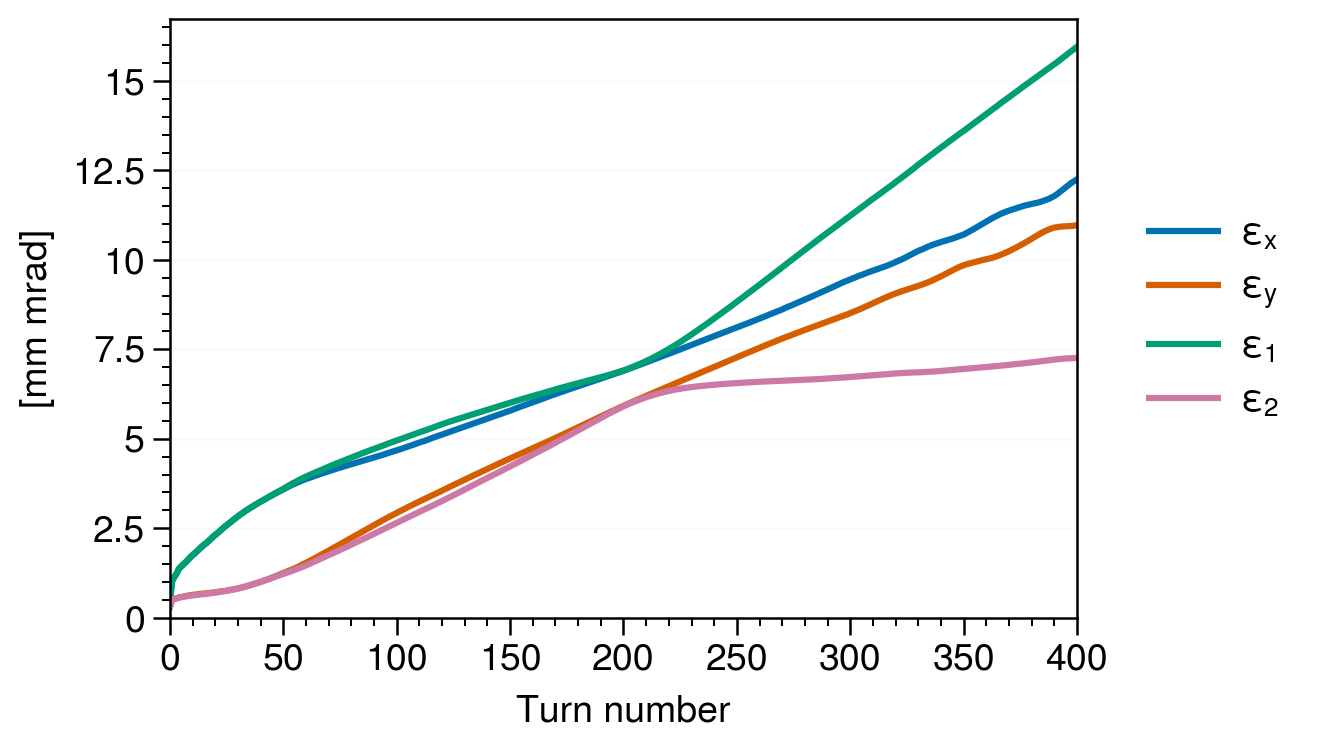
\includegraphics[width=\textwidth]{Images/chapter5/exp3/sim_emittances_nux6.195_nuy6.18.png}
    \end{subfigure}
    \caption{Simulation of Experiment 3 with $\nu_x = 6.195$, $\nu_y = 6.18$.}
    \label{fig:exp3_sim_nux6.195_nuy6.18}
\end{figure}
%
The time at which the intrinsic emittances diverge from the apparent emittances has been pushed towards the end of injection. Although it is difficult to make detailed comparisons between the measurements and the simulations due to possible differences in the ring Twiss parameters at the injection point (resulting in a different beam size for the same kicker settings), uncertainty in the total beam charge, some uncertainty in the measured injection position/angle, and relatively large error bars on the measured emittances, the similarities between the measured emittances in Fig.~\ref{fig:exp3_emittances} and the simulated emittances in Fig.~\ref{fig:exp3_sim_nux6.195_nuy6.18} are striking.\footnote{Although the tune split was measured to be $\approx$ 0.01 with small expected uncertainty $\cite{Pelaia2016}$, the uncertainty in the tune measurement should be re-examined and work should be done to synchronize the ring model in PyORBIT with the online model in OpenXAL. The measurement should also be repeated as the tune split is varied.} These simulations indicate that the elliptical painting method (without solenoids) is very sensitive to the tune split in the ring, which may place a practical lower limit on the 4D emittance at this time; however, the qualitative agreement between measurement and simulation obtained here leaves open the possibility that tuning of the injection region and the addition of solenoid magnetic fields to the ring will bring the beam closer to a self-consistent state.



\section{Summary and additional comparison between experiments}

Let us make two additional comparisons between the final distributions in the three experiments. First, we reconstruct the covariance matrix at different locations in the RTBT. This will not change the emittances but will change the correlations between the phase space coordinates: the smaller the 4D emittance, the larger the variation in these correlations. See Fig.~\ref{fig:exp3_compare_corr}.
%
\begin{figure}[!p]
    \centering
    \vspace*{3.0cm}
    \begin{subfigure}{0.32\textwidth}
        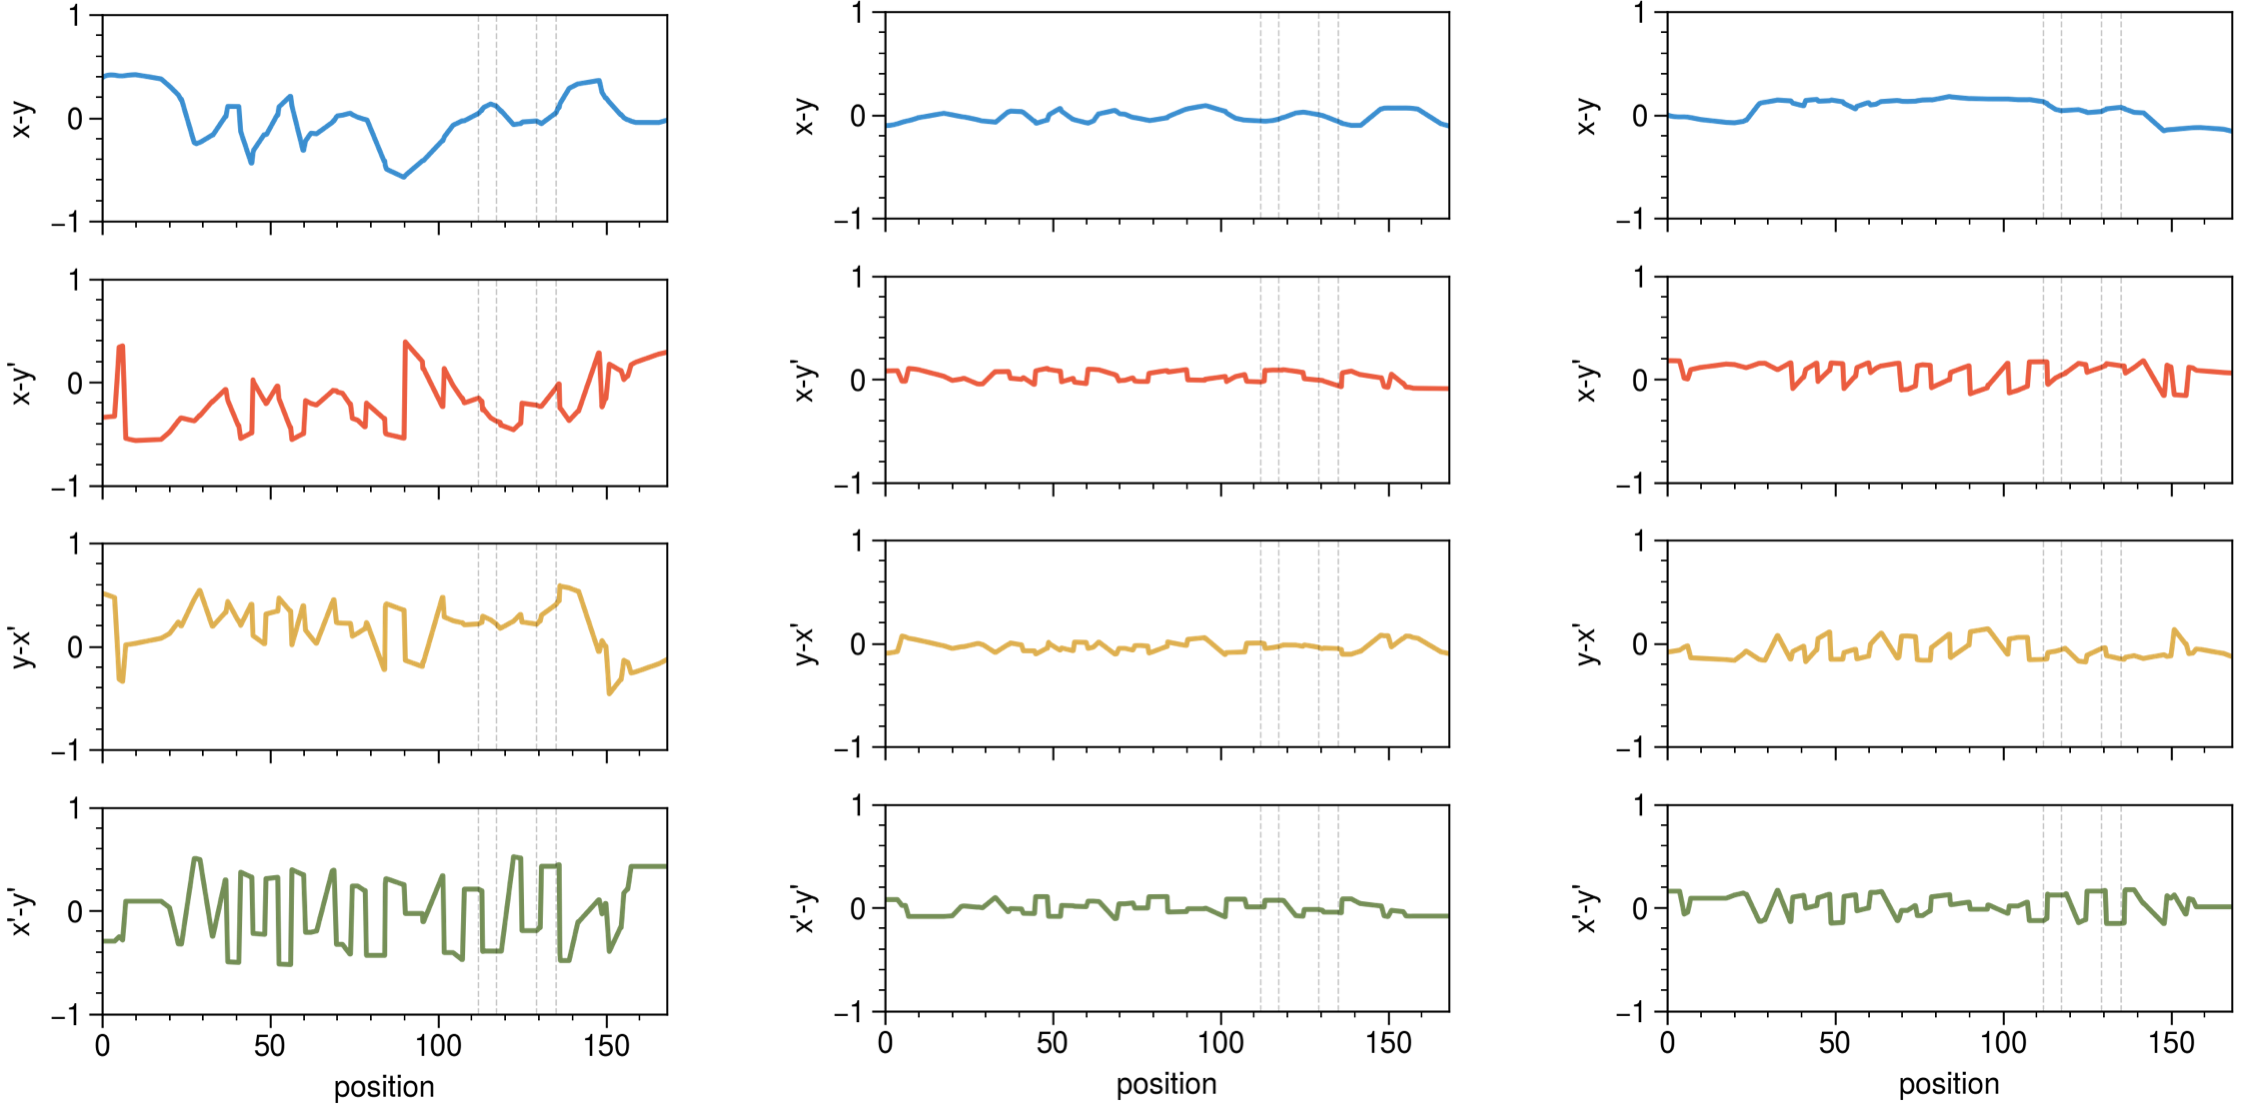
\includegraphics[width=\textwidth]{Images/chapter5/exp3/compare_corr.png}
    \end{subfigure}
    \hfill
    \begin{subfigure}{0.32\textwidth}
        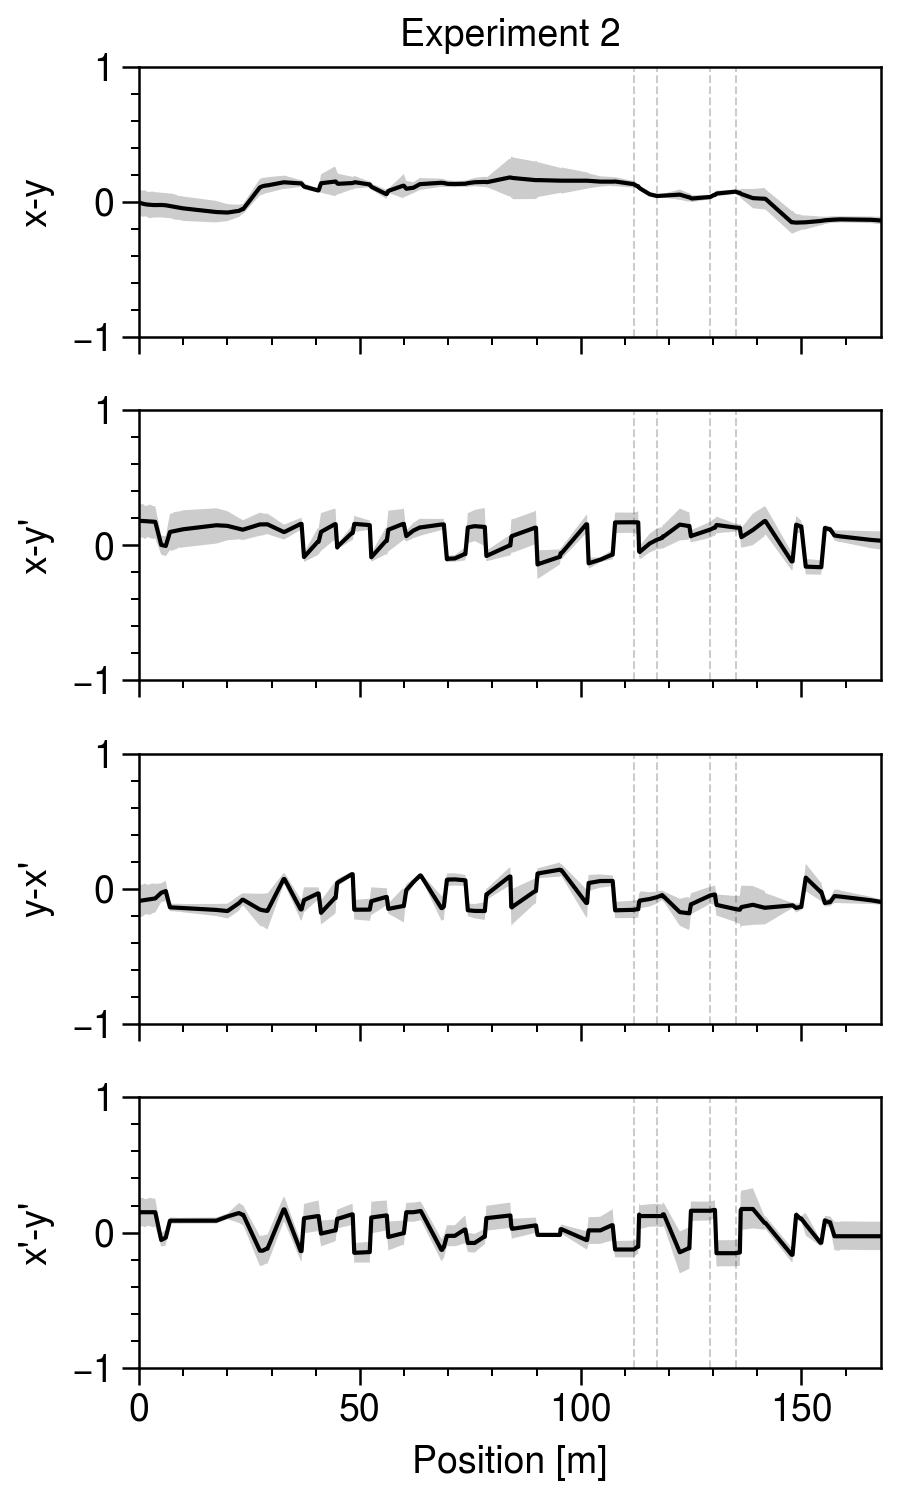
\includegraphics[width=\textwidth]{Images/chapter5/exp2/compare_corr.png}
    \end{subfigure}
    \hfill
    \begin{subfigure}{0.32\textwidth}
        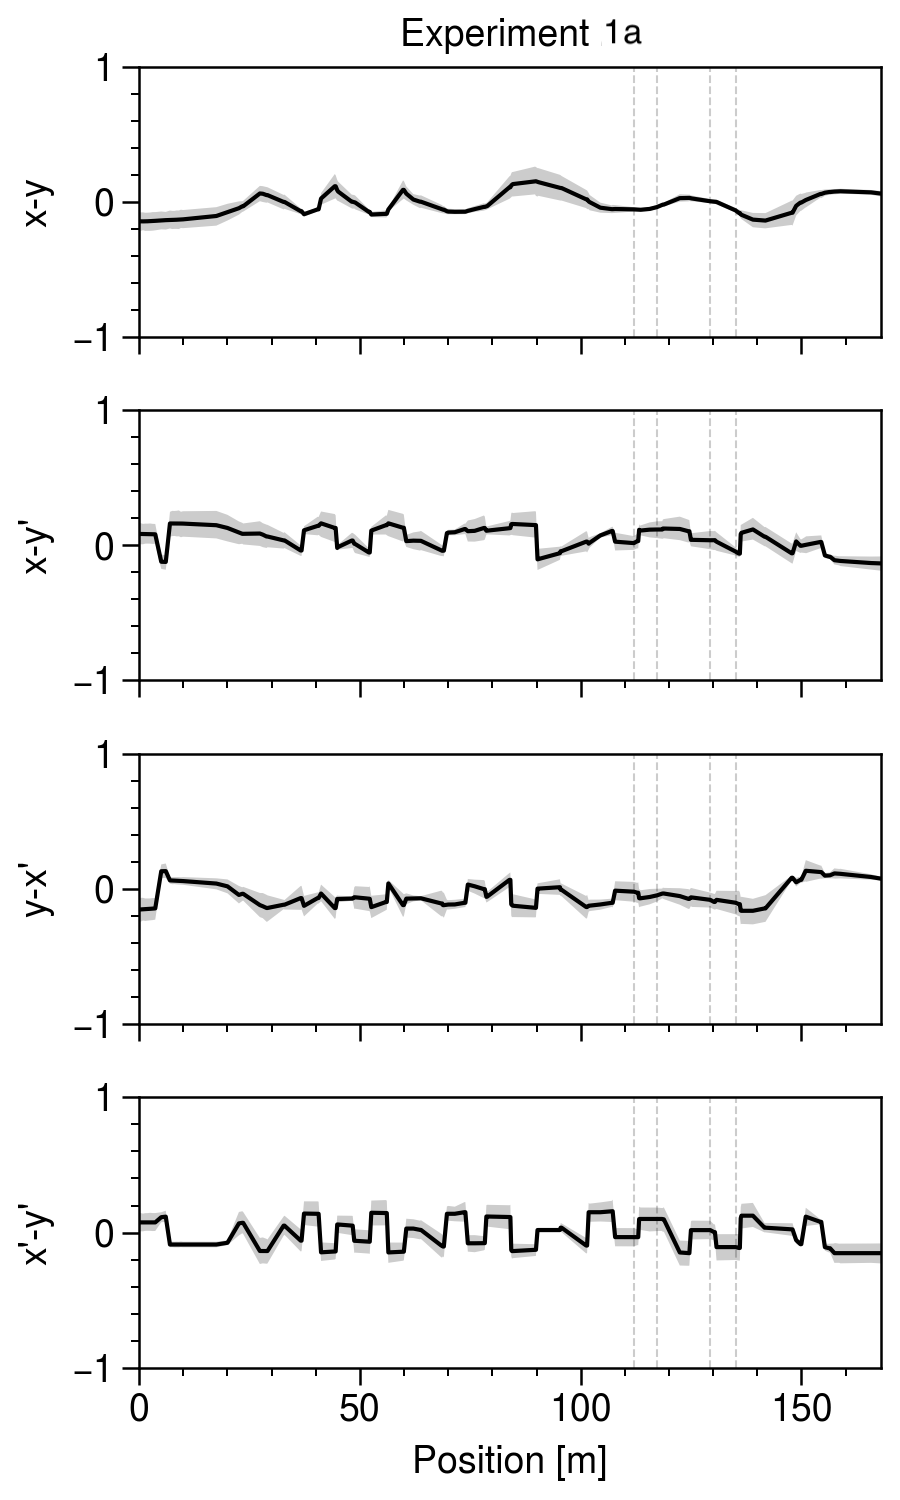
\includegraphics[width=\textwidth]{Images/chapter5/exp1a/compare_corr.png}
    \end{subfigure}
    \caption{Reconstructed cross-plane correlation coefficients for Experiments 3, 2, and 1a.}
    \label{fig:exp3_compare_corr}
    \vspace*{3.0cm}
\end{figure}
% 
The black lines represent the reconstructed values and the grey regions represent the standard deviation. This is simply an alternative way to visualize the measured reduction in 4D emittance in Experiment 3.

Second, although the color histograms in Fig.~\ref{fig:exp1a_wsmeas}, Fig.~\ref{fig:exp1b_wsmeas}, Fig.~\ref{fig:exp2_wsmeas}, and Fig.~\ref{fig:exp3_wsmeas} are useful to show the measured beam evolution in one figure, the 1D profiles may be more difficult to interpret than a normal histogram plot. We therefore include Fig.~\ref{fig:exp1a_fits}, Fig.~\ref{fig:exp1b_fits}, Fig.~\ref{fig:exp2_fits}, and Fig.~\ref{fig:exp3_fits}, which show the final measured wire-scanner profiles from each experiment. Also plotted are the projections of a Gaussian distribution (red) and uniform density elliptical distribution (blue) with the same standard deviation as the RMS calculation from the measurement. 
%
\begin{figure}[!p]
    \centering
    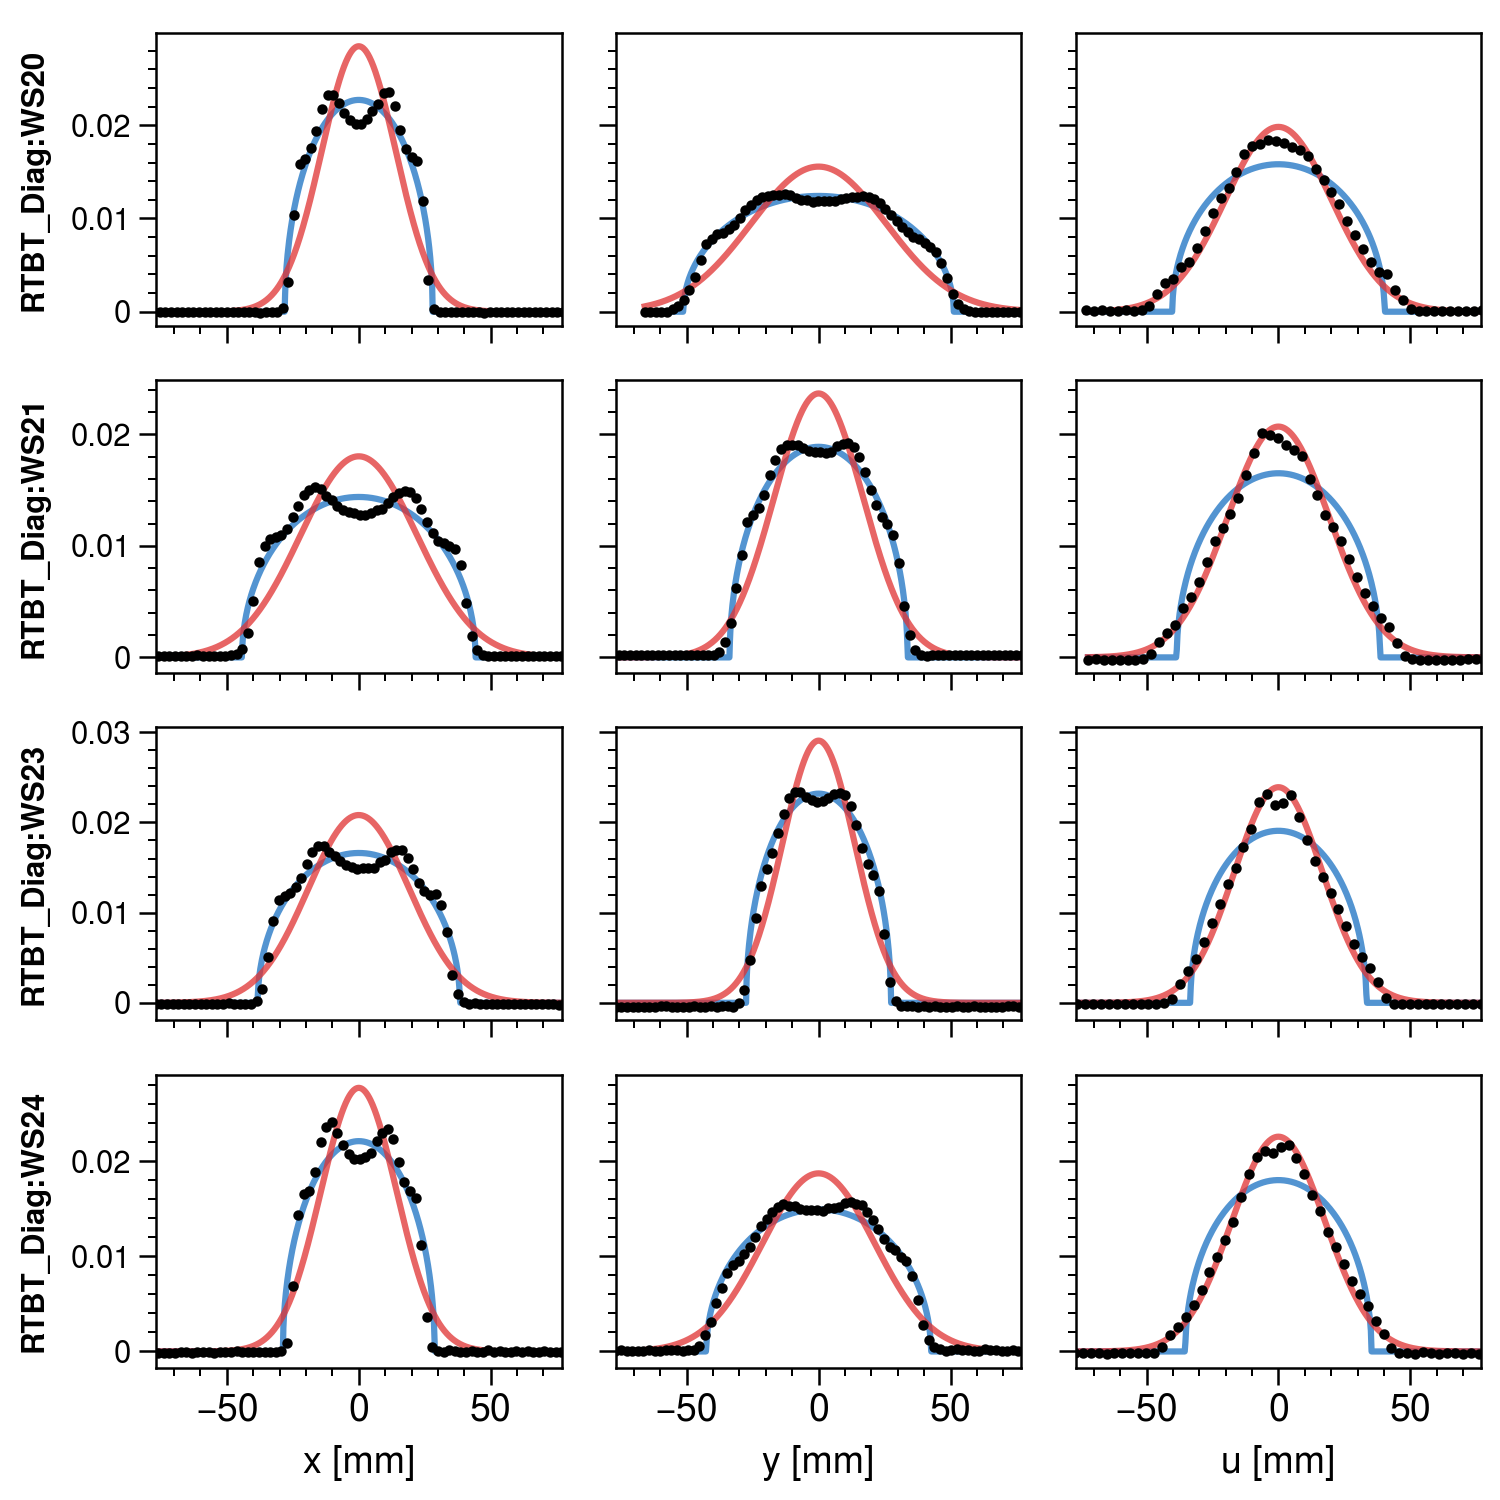
\includegraphics[width=0.9\textwidth]{Images/chapter5/exp1a/fits_9.png}
    \caption{Measured wire-scanner profiles for the final distribution in Experiment 1a. Also plotted are the projections of a Gaussian distribution (red) and uniform density elliptical distribution (blue) with the same standard deviation as the rms calculation from the measurement.}
    \label{fig:exp1a_fits}
\end{figure}
%
\begin{figure}[!p]
    \centering
    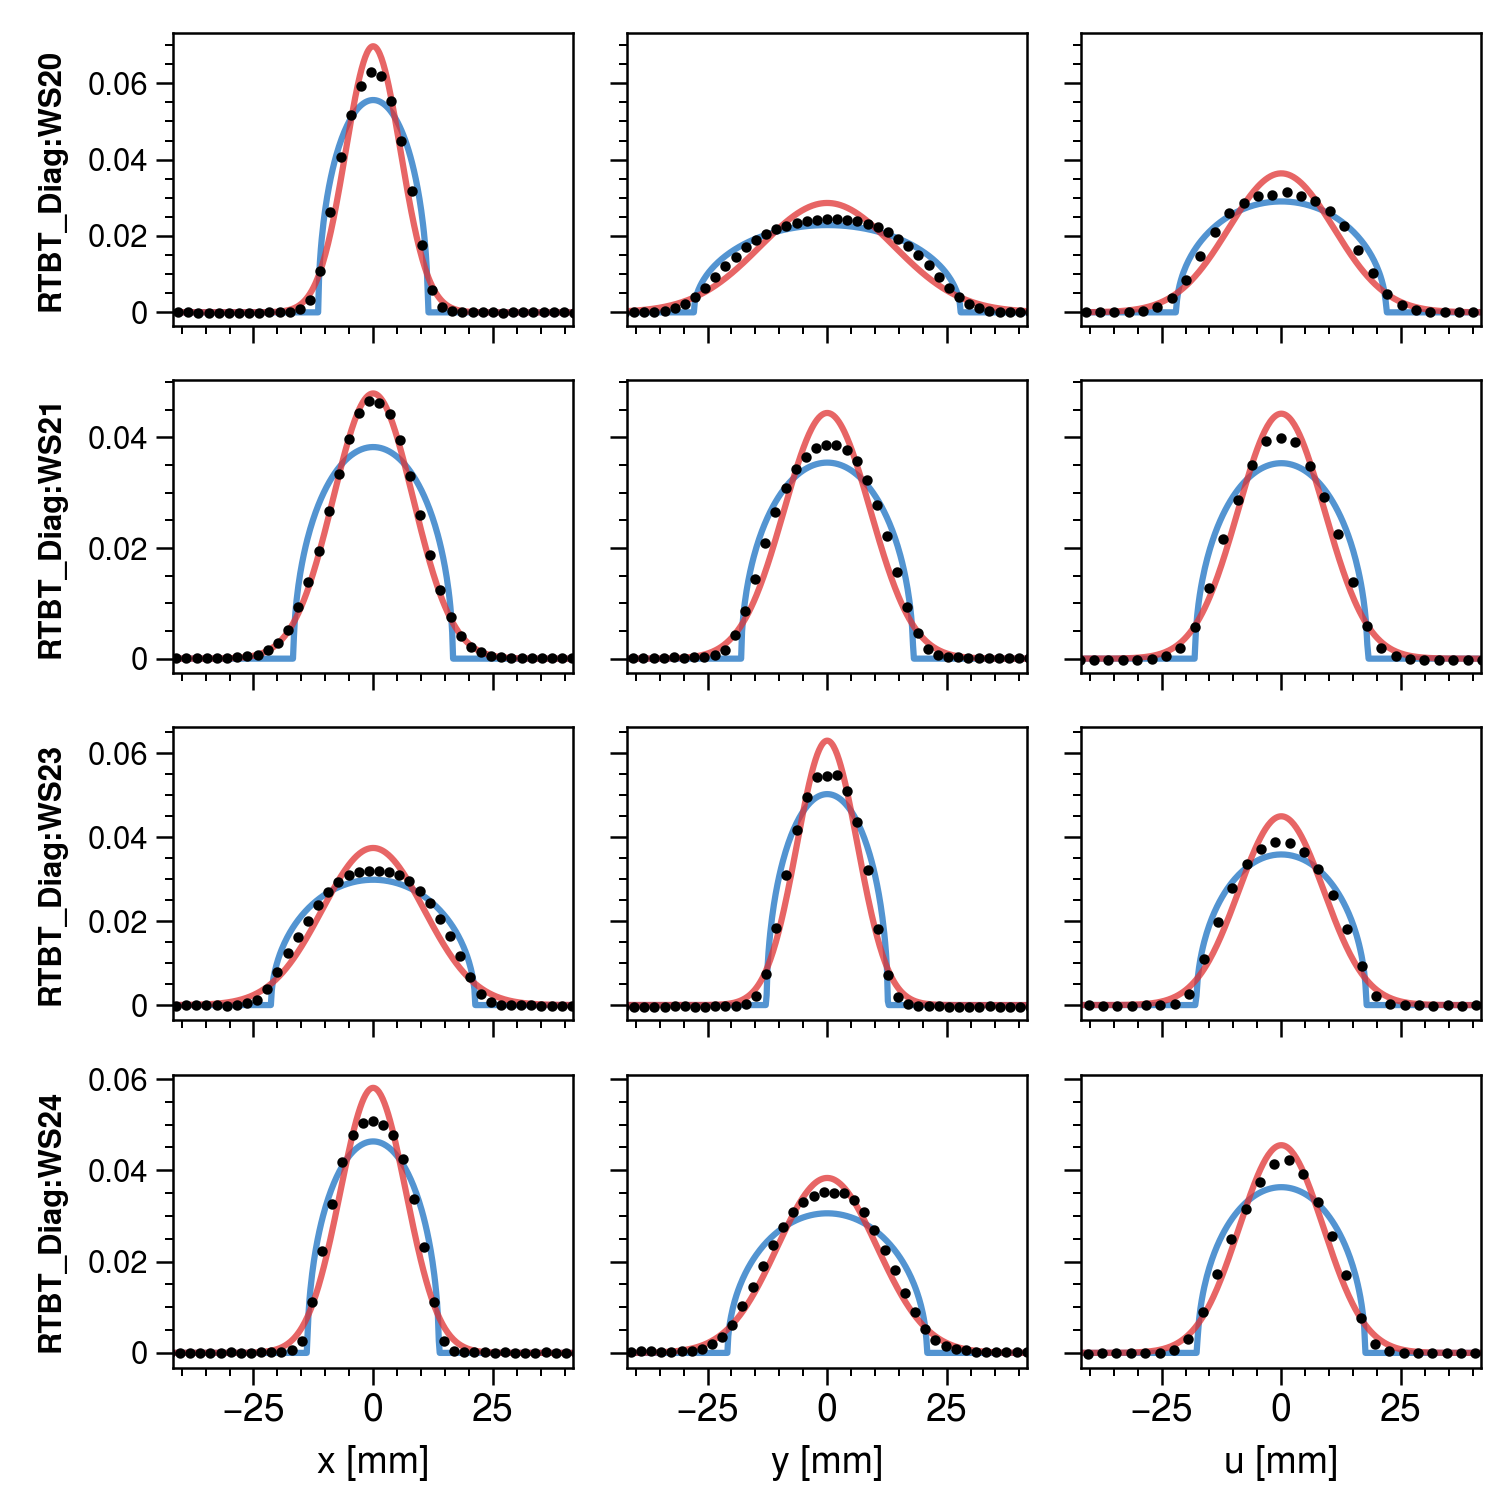
\includegraphics[width=0.9\textwidth]{Images/chapter5/exp1b/fits_9.png}
    \caption{Measured wire-scanner profiles for the final distribution in Experiment 1b.}
    \label{fig:exp1b_fits}
\end{figure}
%
\begin{figure}[!p]
    \centering
    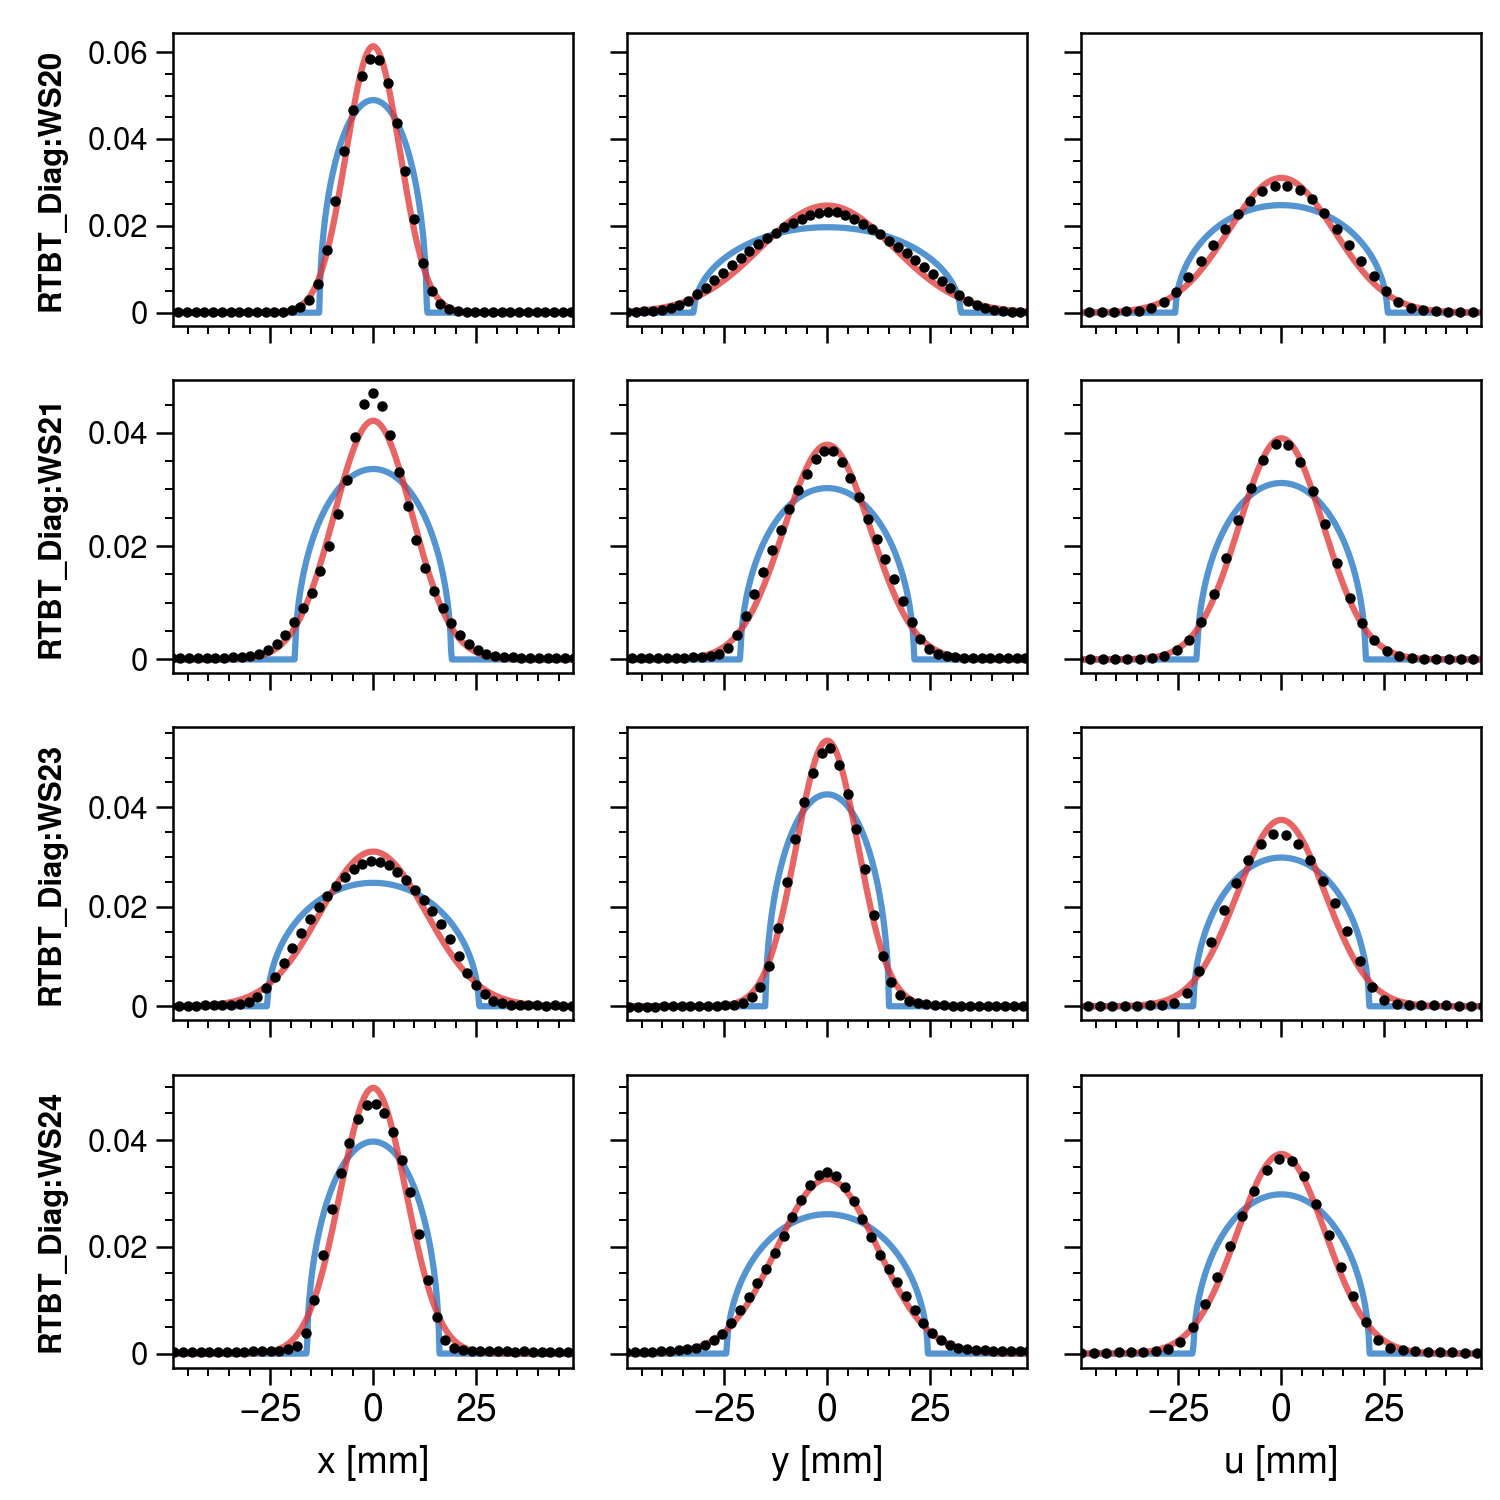
\includegraphics[width=0.9\textwidth]{Images/chapter5/exp2/fits_9.png}
    \caption{Measured wire-scanner profiles for the final distribution in Experiment 2.}
    \label{fig:exp2_fits}
\end{figure}
%
\begin{figure}[!p]
    \centering
    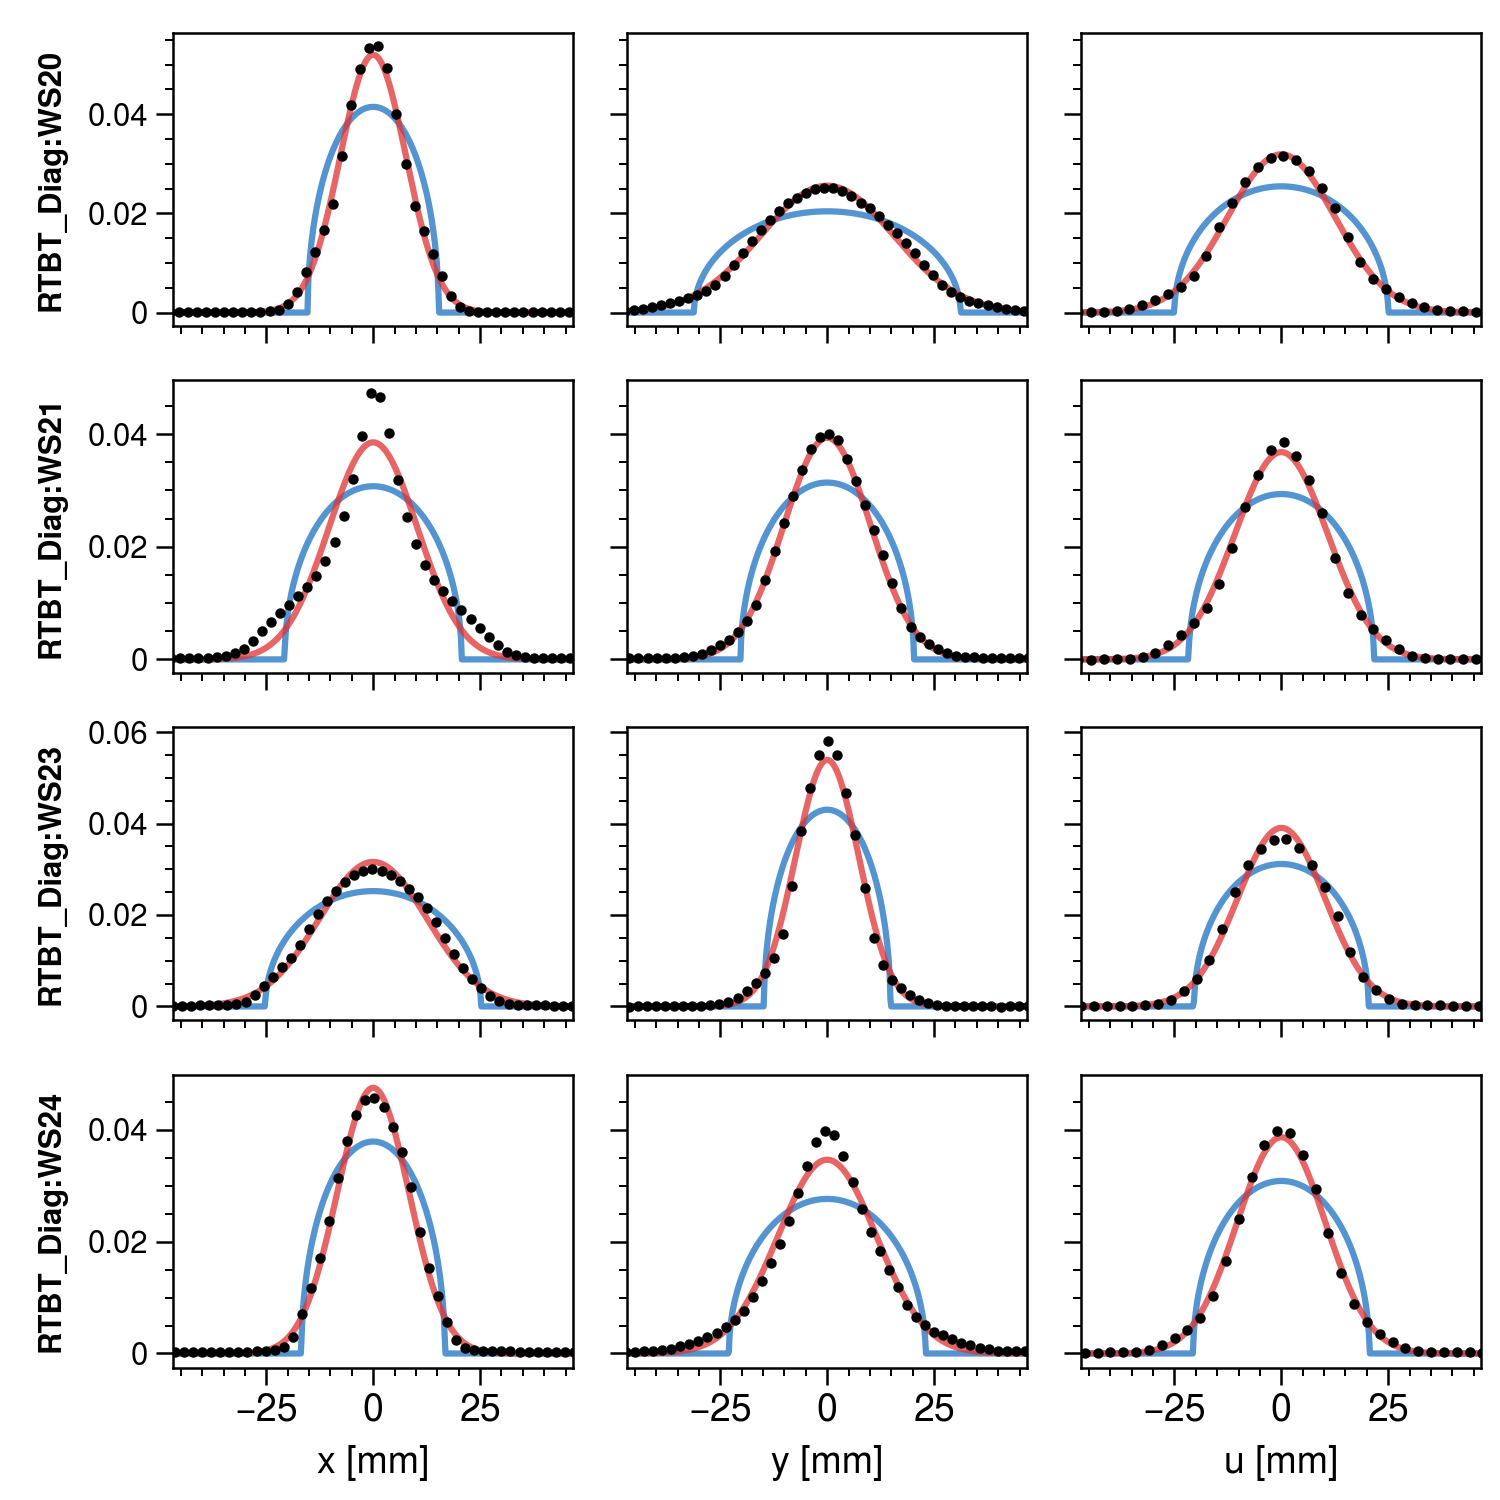
\includegraphics[width=0.9\textwidth]{Images/chapter5/exp3/fits_7.png}
    \caption{Measured wire-scanner profiles for the final distribution in Experiment 3.}
    \label{fig:exp3_fits}
\end{figure}
%

We now review the main results of the experiments in this chapter, commenting on these wire-scanner profiles along the way. Recall that our goal was to carry out the elliptical painting method in the SNS, measure the painted distribution, and compare the measurements to an ideal Danilov distribution. This has been accomplished. 

In Experiment 1, the Ring Injection Control (RIC) application was tested at 1 GeV beam energy, and the beam emittance was efficiently measured throughout injection. First, correlated painting was used in Experiment 1a; the measured intrinsic emittances remained close to the apparent emittances, showing that there was very little cross-plane correlation in the beam. Second, in Experiment 1b, it was found that lowering the beam energy was necessary to inject particles onto the closed orbit, which is a necessary condition to perform the elliptical painting method. Nonetheless, setting equal tunes in the ring and varying the vertical injection angle resulted in a measured split in the intrinsic emittances. Furthermore, some of the measured wire-scanner profiles were more consistent with the projection of a uniform density elliptical distribution than with a Gaussian distribution. This gave us confidence that RIC was working as intended.

In Experiment 2, the beam energy was lowered to 0.8 GeV. BPM measurements verified that the initial kicker settings could be achieved so that particles were injected onto the closed orbit. The final kicker settings were chosen so that ($x$, $x'$, $y$, $y'$) $\approx$ (21 mm, 0 mrad, 0 mmm, 1.1 mrad). Wire-scanner measurements showed that the beam size grew with approximate square root time-dependence, as intended, but only a small split in the intrinsic emittances was measured at the end of injection. Additionally, the wire-scanner profiles were more consistent with a Gaussian distribution.

In Experiment 3, the beam size and intensity were varied. The most promising case — 20\% reduction in beam intensity and 50\% increase in horizontal beam size — was investigated in more detail. A larger split in the intrinsic emittances was measured during the last hundred turns of injection. Additionally, the tilt angle of the beam image on the target was shown to depend on the phase advances at the target (even though the bunch length was inadvertently reduced). Although most of the wire-scanner profiles still appeared to be consistent with a Gaussian distribution, one could argue that there were subtle differences from the previous experiment. For example, in Fig.~\ref{fig:exp3_fits}, the horizontal projection at WS21 exhibits a sharp peak, resembling the $y'$ projection in Fig.~\ref{fig:Holmes}. (This is also present at WS20 to a lesser extent.) These features only appeared after 300 turns, when the intrinsic emittances began to split. Finally, simulations were performed to reproduce the measured emittance growth during injection. By splitting the tunes by 0.015 in the simulation, the qualitative behavior of the emittance growth was reproduced. This showed that the distribution is quite sensitive to the tune split in the ring.

These results are promising: extensive troubleshooting has occurred during machine setup, the ring orbit has been measured and controlled, and modifications to the machine have been shown to have a positive effect on the painted distribution. Furthermore, the simulation-measurement agreement in Experiment 3 offers hope that future optimization of the SNS will result in the production of a Danilov-like distribution in the ring. One immediate need is to modify the injection region to increase the maximum vertical injection angle so that a larger, rounder beam can be painted.